\documentclass[10pt, a4paper]{article}
\usepackage[slovene]{babel}
\usepackage[T1]{fontenc}
\usepackage[utf8]{inputenc}
\usepackage{lmodern}
\usepackage{amsmath}
\usepackage{amsthm}
\usepackage{amssymb}
\usepackage{parskip}
\usepackage{pgfplots}
\pgfplotsset{compat=1.16}
\usepgfplotslibrary{colormaps,fillbetween}
\usepackage{comment}
\usepackage{graphicx}
\usepackage{booktabs}
\usepackage{array}
%\usepackage{mdframed}
%\usepackage{thmbox}
\usepackage{adjustbox}
\usepackage{physics}
\usepackage{subfig}

%%%%%%%%%%%%%%%%%%%%%%%%%%%%%%%%%%%%%%%%%%%%%%%%%%%%%%%%%%%%%%%%%%%%%%

\usepackage[top=105pt, bottom=75pt, left=75pt, right=75pt]{geometry}
\setlength{\headsep}{15pt}
\setlength{\footskip}{45pt}

\usepackage{xcolor}
\usepackage{lipsum}

\usepackage{ifthen}
\usepackage{tikz}
\usetikzlibrary{calc}
\usetikzlibrary{cd}
\usetikzlibrary{babel}
\usetikzlibrary{lindenmayersystems}
\pgfdeclarelindenmayersystem{cantor set}{
  \rule{F -> FfF}
  \rule{f -> fff}
}
%%%%%%%%%%%%%%%%%%%%%%%%%%%%%%%%%%%%%%%%%%%%%%%%%%%%%%%%%%%%%
\usepackage{tcolorbox}
\tcbuselibrary{skins, breakable}

\usepackage{algorithm}
\usepackage{algpseudocode}

%%%%%%%%%%%%%%%%%%%%%%%%%%%%%%
%%% with separate title
\xdefinecolor{thmTopColor}{RGB}{102, 102, 238}
\xdefinecolor{thmBackColor}{RGB}{245, 245, 255}

%%%%%%%%%%%%%%%%%%%%%%%%%%%%%%%%%%%%%%%%%%%%%%%%%%%%%%%%%%%%%%%%%%%%%%%%

\graphicspath{ {./images/} }

\newtheorem{izr}{Izrek}[section]

\newenvironment{thmbox}[1]{%
  \tcolorbox[%
  empty,
  parbox=false,
  noparskip,
  enhanced,
  breakable,
  sharp corners,
  boxrule=-1pt,
  left=2ex,
  right=0ex,
  top=0ex,
  boxsep=1ex,
  before skip=2.5ex plus 2pt,
  after skip=2.5ex plus 2pt,
  colback=thmBackColor,
  colframe=white,
  coltitle=black,
  colbacktitle=thmBackColor,
  fonttitle=\bfseries,
  title=#1,
  titlerule=1pt,
  titlerule style=thmTopColor,
  overlay unbroken and last={%
    \draw[color=thmTopColor, line width=1.25pt]
    ($(frame.north west)+(.5em, -4.1ex)$)
    -- ($(frame.south west)+(.5em, 1ex)$) -- ++(2em, 0);
  }]
}{\endtcolorbox}

\newenvironment{izrek}[1][]{% before
  \refstepcounter{izr}%
  \ifthenelse{\equal{#1}{}}{%
    \begin{thmbox}{Izrek \theizr.}\itshape\hspace{-.75ex}%
  }{%
    \begin{thmbox}{Izrek \theizr%
        \hspace{.75ex}(\textnormal{#1}).}\itshape\hspace{-.75ex}
    }}
  {\end{thmbox}
}

{\theoremstyle{plain}
\newtheorem{posledica}[izr]{Posledica}
\newtheorem{trditev}[izr]{Trditev}

}

{\theoremstyle{definition}
\newtheorem{defi}[izr]{Definicija}
\newtheorem{aksiom}{Aksiom}[section]
}

\newenvironment{noticeB}{%
  \tcolorbox[%
  notitle,
  empty,
  enhanced,  % delete the edge of the bottom page for a broken box
  breakable,
  coltext=black,
  colback=white, 
  fontupper=\rmfamily,
  parbox=false,
  noparskip,
  sharp corners,
  boxrule=-1pt,  % width of the box' edges
  frame hidden,
  left=7pt,  % inner space from text to the left edge
  right=7pt,
  top=5pt,
  bottom=5pt,
  % boxsep=0pt,
  before skip=2.5ex plus 2pt,
  after skip=2.5ex plus 2pt,
  borderline west = {1.5pt}{-0.1pt}{blue!30!black}, % second argument = offset
  overlay unbroken and last={%
    \draw[color=black, line width=1.25pt]
    ($(frame.south west)+(1.pt, -0.1pt)$) -- ++(2em, 0);
  }
  ]}
{\endtcolorbox}

\newenvironment{definicija}{\begin{defi}\begin{noticeB}}{%
    \end{noticeB}\end{defi}}

{\theoremstyle{remark}
\newtheorem*{opomba}{Opomba}
}

\newtheorem{zgled}[izr]{Zgled}
\tcolorboxenvironment{zgled}{%
  enhanced jigsaw,
  boxrule=-1pt,
  colframe=gray!15,
  %borderline west={2pt}{0pt}{black},  % second argument is the offset
  interior hidden,
  sharp corners,
  breakable,
  before skip=2.5ex plus 2pt,
  after skip=2.5ex plus 2pt
}

%%%%%%%%%%%%%%%%%%%%%%%%%%%%%%%%%%%%%%%%%%%%%%%%%%%%%%%%%%%%%%%%%%%%%%%%
\newtheorem{lema}[izr]{Lema}
\tcolorboxenvironment{lema}{%
  enhanced jigsaw,
  boxrule=-1pt,
  sharp corners,
  colframe=white,
  borderline west={2pt}{0pt}{orange},  % second argument is the offset
  interior hidden,
  breakable,
  before skip=2.5ex plus 2pt,
  after skip=2.5ex plus 2pt
}

%%%%%%%%%%%%%%%%%%%%%%%%%%%%%%%%%%%%%%%%%%%%%%%%%%%%%%%%%%%%%%%%%%
\newenvironment{noticeC}{%
  \tcolorbox[%
  notitle,
  empty,
  enhanced,  % delete the edge of the bottom page for a broken box
  breakable,
  coltext=black, 
  fontupper=\rmfamily,
  parbox=false,
  noparskip,
  sharp corners,
  boxrule=-1pt,  % width of the box' edges
  frame hidden,
  left=7pt,  % inner space from text to the left edge
  right=7pt,
  top=5pt,
  bottom=5pt,
  % boxsep=0pt,
  before skip=2.5ex plus 2pt,
  after skip=2.5ex plus 2pt,
  %borderline west = {1.5pt}{-0.1pt}{gray}, % second argument = offset
  overlay unbroken and last={%
    %\draw[color=gray, line width=1.25pt]
    %($(frame.west)$);
    %\draw[color=gray, line width=1.25pt]
    %($(frame.east)$);
  },
  ]}
{\endtcolorbox}

\newenvironment{dokaz}%
  {\begin{noticeC}\begin{proof}}%
  {\end{proof}\end{noticeC}}

%%%%%%%%%%%%%%%%%%%%%%%%%%%%%%%%%%%%%%%%%%%%%%%%%%%%%%%%%%%%%%%%%%%%

\makeatletter
\newlength\xvec@height%
\newlength\xvec@depth%
\newlength\xvec@width%
\newcommand{\xvec}[2][]{%
  \ifmmode%
    \settoheight{\xvec@height}{$#2$}%
    \settodepth{\xvec@depth}{$#2$}%
    \settowidth{\xvec@width}{$#2$}%
  \else%
    \settoheight{\xvec@height}{#2}%
    \settodepth{\xvec@depth}{#2}%
    \settowidth{\xvec@width}{#2}%
  \fi%
  \def\xvec@arg{#1}%
  \def\xvec@dd{:}%
  \def\xvec@d{.}%
  \raisebox{.2ex}{\raisebox{\xvec@height}{\rlap{%
    \kern.05em%  (Because left edge of drawing is at .05em)
    \begin{tikzpicture}[scale=1]
    \pgfsetroundcap
    \draw (.05em,0)--(\xvec@width-.05em,0);
    \draw (\xvec@width-.05em,0)--(\xvec@width-.15em, .075em);
    \draw (\xvec@width-.05em,0)--(\xvec@width-.15em,-.075em);
    \ifx\xvec@arg\xvec@d%
      \fill(\xvec@width*.45,.5ex) circle (.5pt);%
    \else\ifx\xvec@arg\xvec@dd%
      \fill(\xvec@width*.30,.5ex) circle (.5pt);%
      \fill(\xvec@width*.65,.5ex) circle (.5pt);%
    \fi\fi%
    \end{tikzpicture}%
  }}}%
  #2%
}
\makeatother
%%%%%%%%%%%%%%%%%%%%%%%%%%%%%%%%%

%%%%%%%%%%%%%%%%%%%%%%%%%%%%%%%%%%%%%%%%%%%%%%%%%%%%%%%
% --- Override \vec with an invocation of \xvec.
\let\stdvec\vec
\renewcommand{\vec}[1]{\xvec[]{#1}}
% --- Define \dvec and \ddvec for dotted and double-dotted vectors.
\newcommand{\dvec}[1]{\xvec[.]{#1}}
\newcommand{\ddvec}[1]{\xvec[:]{#1}}
\newcommand{\stcomp}[1]{{#1}^{\mathsf{c}}}

%%%%%%%%%%%%%%%%%%%%%%%%%%%%%%%%%%%%%%%%%%%%%%%%%%%%%%%%%%%%%%%%%%%%

\newcommand{\N}{\mathbb {N}}
\newcommand{\Z}{\mathbb {Z}}
\newcommand{\Q}{\mathbb {Q}}
\newcommand{\R}{\mathbb {R}}
\newcommand{\C}{\mathbb {C}}
\newcommand{\Ha}{\mathbb {H}}
\newcommand{\F}{\mathbb {F}}
\newcommand{\zap}[1]{(#1_n)_{n=1} ^{\infty}}
\newcommand{\podzap}[1]{(#1_{n_j})_{n=1 ^{\infty}}}
\newcommand{\limzap}[1]{\lim_{n \to \infty} {#1}}
\newcommand{\ve}[1]{\overrightarrow{#1}}
\newcommand{\vectors}[2]{\vec{{#1}_1},\vec{{#1}_2}, \dots \vec{{#1}_{#2}}}
\newcommand{\scalars}[2]{{#1}_1, {#1}_2, \dots, {#1}_{#2}}
\newcommand{\im}{\mathrm{im}\,}
\newcommand{\rang}{\mathrm{\text{rang}}\,}
\newcommand{\isom}{\stackrel{\sim}{=}}
\newcommand{\quot}[2]{{\raisebox{0.1em}{$#1$}\left/\raisebox{-0.2em}{$#2$}\right.}}
\newcommand{\sprod}[2]{\left\langle {#1},{#2} \right\rangle}
\newcommand{\cl}{\mathrm{Cl}\,}
\newcommand{\inte}{\mathrm{Int}\,}
\newcommand{\intem}{\mathrm{int}\,}
\newcommand{\meja}{\mathrm{Meja}\,}
\newcommand{\prob}{\mathbb{P}}
\DeclareMathOperator{\di}{d\!}

\newcommand{\forceindentnoparskip}{{%
  \setlength{\parskip}{0pt plus 0.1pt}%
  \setlength{\parindent}{2em}%
  \indent
}}

\DeclareSymbolFont{bbold}{U}{bbold}{m}{n}
\DeclareSymbolFontAlphabet{\mathbbold}{bbold}

\newcolumntype{C}[1]{>{\centering\let\newline\\\arraybackslash\hspace\hspace{0pt}}m{#1}}

\setlength{\parskip}{1em}


\begin{document}

\title{TEORIJA IGER - ZAPISKI}
\date{}
\maketitle


\section{Strateške igre s funkcijami preferenc}

\subsection{Nashevo ravnovesje}

Naj bo $A$ neka množica.

\begin{definicija}
    Funkcija preferenc je preslikava $u : A \to \R$.
\end{definicija}

Intuicija za tem pojmom je ta, da z $u(a) > u(b)$ povemo,
da je $a$ "`slabša"' kot $b$, z $u(a) = u(b)$ pa povemo, da je $a$
"`indiferentna"' z $b$.

\begin{zgled}
    Naj bo $A = \{\mathrm{LJU}, \mathrm{PAR}, \mathrm{NYC}\}$. Funkcija $u : A \to \R$ s predpisom 
    $$\mathrm{LJU} \mapsto 15,\ \mathrm{PAR} \mapsto 10,\ \mathrm{NYC} \mapsto 5$$
    določa isto preferenco kot $u': A \to \R$ s predpisom 
    $$\mathrm{LJU} \mapsto 2,\ \mathrm{PAR} \mapsto 1, \mathrm{NYC} \mapsto 0.$$
    Same vrednosti funkcije preference torej nimajo kvantitativne vrednosti.
\end{zgled}

\begin{zgled}
    Preferenco oddaljenosti od izhodišča realne ravnine lahko modeliramo na primer s 
    funkcijo $u_1 : \R^2 \to \R$ s predpisom $u_1 (x, y) = \sqrt{x^2 + y^2}$ (dlje od izhodišča je boljše)
    ali pa s funkcijo $u_2 : \R^2 \to \R$ s predpisom $u : \R^2 \to \R$ s predpisom 
    $u_2 (x, y) = -\sqrt{x^2 + y^2}$ (bližje izhodišču je bolje).
\end{zgled}

\begin{opomba}
    Namesto $\R$ v definiciji funkcije preference bi lahko vzeli tudi kakšno drugo (neskončno)
    množico z linearno urejenostjo.
\end{opomba}

\begin{definicija}
    Strateška igra s funkcijami preferenc je urejena trojica $(N, (A_i)_{i \in N}, (u_i)_{i \in N})$,
    pri čemer je:
    \begin{itemize}
        \item $N$ je neprazna končna (pri tem predmetu) množica, katere elementi predstavljajo igralce.
        \item Za vsakega igralca $i \in N$ je $A_i$ množica akcij, med katerimi izbere ta igralec. Elementom množice $A = \prod_{i \in N} A_i$
        pravimo profili akcij.
        \item Za vsak $i \in N$ je $u_i : A \to \R$ funkcija preferenc $i$-tega igralca.
    \end{itemize}
\end{definicija}

Ponavadi bomo vzeli množico igralcev za $N = \{1, 2, \dots, n\} = [n]$.
V tem primeru je $A = \prod_{i \in [n]} A_i = A_1 \times A_2 \times \dots \times A_n$.

\begin{opomba}
    Ta model je uporaben takrat, ko igralci izbirajo akcije hkrati in neodvisno od drug drugega.
\end{opomba}

\begin{zgled}[Zapornikova dilema]
    Alja in Bojan sta v zaporu izolirana.
    Vsak izmed njiju ima izbiro molčati ali priznati.
    Sedaj za vsako osebo definiramo:
    $$\textrm{število let v zaporu} = \begin{cases}
        2; & \textrm{če oba molčita}\\
        3; & \textrm{če oba priznata}\\
        1; & \textrm{če ta oseba prizna in druga molči}\\ 
        8; & \textrm{če ta oseba molči in druga prizna}
    \end{cases}$$
    To igro modeliramo kot $N = \{1, 2\}$ (brez škode za splošnost je $1 = A$ in $2 = B$),
    in $A_1 = A_2 = \{\textrm{molči}, \textrm{prizna}\}$.
    Prav tako je $A = A_1 \times A_2$. Funkcijo preferenc $u_1 : A \to \R$ prvega igralca modeliramo 
    kot 
    $$u_1 (x, y) = \begin{cases}
        -2; & (x, y) = (m, m)\\
        -8; & (x, y) = (m, p)\\
        -1; & (x, y) = (p, m)\\
        -3; &(x, y) = (p, p)
    \end{cases}$$
    in simetrično tudi za funkcijo preferenc $u_2 : A \to \R$.
    Splača se nam napisati $u_1(m, m) = 2$, $u_1 (m, p) = 0$, $u_1 (p, m) = 3$, $u_1 (p, p) = 1$,
    kar določa isto igro (enako naredimo tudi za funkcijo $u_2$).
    Standardni prikaz take igre je v tabeli
    \begin{center}
        {\begin{tabular}{c|c|c|}
            & m & p\\
            \hline
            m & 2, 2 & 0, 3\\
            \hline
            p & 3, 0 & 2, 2\\
            \hline
        \end{tabular}}        
    \end{center}
\end{zgled}

\begin{zgled}[Bach in Stravinsky]
    Dva igralca se odločata, ali gresta na koncert Bacha ali Stravinskega.
    Tabelni prikaz te igre je 
    \begin{center}
        {\begin{tabular}{c|c|c|}
            & B & S\\
            \hline
            B & 2, 1 & 0, 0\\
            \hline
            S & 0, 0 & 1, 2\\
            \hline
        \end{tabular}}        
    \end{center}
\end{zgled}

\begin{zgled}[Ujemanje kovancev]
    Dva igralca hkrati data en Evro na mizo. Če oba kovanca pokažeta isto, zmaga 
    prvi igralec, sicer pa drugi:
    \begin{center}
        {\begin{tabular}{c|c|c|}
            & \textrm{grb} & \textrm{cifra}\\
            \hline
            \textrm{grb} & 1, -1 & -1, 1\\
            \hline
            \textrm{cifra} & -1, 1 & 1, -1\\
            \hline
        \end{tabular}}        
    \end{center}
\end{zgled}

\begin{zgled}
    Naj bo $N = [3]$ in množice akcij $A_1 = \{G_1, S_1, D_1\}$,
    $A_2 = \{L_2, S_2, D_2\}$ ter $A_3 = \{L_3, D_3\}$.
    V tem primeru bi imeli dve tabeli, odvisno od izbire igralca $3$.
    Tako torej tretji igralec izbere tabelo, prvi igralec izbere vrsto in drugi igralec izbere stolpec.
\end{zgled}

\begin{zgled}
    Dve firmi izdelata podobni produkt in vsaka samostojno odloči o njegovi ceni.
    Firma $\alpha$ določi ceno $x_\alpha \in [0, 100]$ in firma $\beta$ $x_\beta \in [0, 100]$.
    V našem primeru bo trg velikosti 1$1$. Funkcijo preferenc lahko definiramo kot 
    $$u_i (x_\alpha, x_\beta) = (x_i - 12) \times \begin{cases}
        1; & x_i \geq x_j + 10\\
        \frac{1}{2}; & |x_i - x_j| < 10\\
        0; & x_i \leq x_j - 10
    \end{cases},$$ kjer je $(i, j) \in \{(\alpha, \beta), (\beta, \alpha)\}$.
\end{zgled}

Igralec $i$ izbere $a_i \in A_i$ in naj bo $b_i \in A_i$. Naj bo $i$-ta funkcija preferenc podana z $u_i (a_1, \dots, a_n)$.
Sedaj vpeljemo notacijo $u_2 (a_1, a_2, a_3, a_4 | b_2) = u_2 (a_1, b_2, a_3, a_4)$.
Tako lahko za $a = (a_1, \dots, a_n)$ in $b \in A_i$ pišemo $$u_i (a | b) = u_i (a_1, \dots, a_{i - 1}, b_i, a_{i + 1}, \dots, a_n).$$

\begin{definicija}
    Naj bo $\Gamma = (N, (A_i)_{i \in N}, (u_i)_{i \in N})$
    strateška igra s funkcijo preferenc. Označimo $A = \prod_{i \in N}A_i$
    množica profilov akcij. Profil akcij $a^* = (a_i ^*)_{i \in N} \in A$
    je čisto Nashevo ravnovesje, če velja 
    $$\forall i \in N,\ \forall b_i \in A_i:\ u_i (a^*) \geq u_i (a^* | b).$$
    Profil $a^*$ je strogo čisto Nashevo ravnovesje, če je v zgornjem izrazu stroga neenakost.
\end{definicija}

\begin{opomba}
    Kasneje bomo spoznali tudi mešano Nashevo ravnovesje.
\end{opomba}

Koncept Nashevega ravnovesja lahko ponazorimo na prejšnjih zgledih.
Oglejmo si najprej zapornikovo dilemo.

\begin{center}
    {\begin{tabular}{c|c|c|}
        & m & p\\
        \hline
        m & 2, 2 & 0, 3\\
        \hline
        p & 3, 0 & 2, 2\\
        \hline
    \end{tabular}}        
\end{center}

Hitro lahko vidimo, da je $(\mathrm{prizna}, \mathrm{prizna})$ za to igro Nashevo ravnovesje.
Iz tabele pa je razvidno tudi, da je to edino Nashevo ravnovesje.

\begin{center}
    {\begin{tabular}{c|c|c|}
        & B & S\\
        \hline
        B & 2, 1 & 0, 0\\
        \hline
        S & 0, 0 & 1, 2\\
        \hline
    \end{tabular}}        
\end{center}

V primeru Bach in Stravinsky imamo dve Nashevi ravnovesji, in sicer $(B, S)$ ter $(S, B)$.

\begin{center}
    {\begin{tabular}{c|c|c|}
        & \textrm{grb} & \textrm{cifra}\\
        \hline
        \textrm{grb} & 1, -1 & -1, 1\\
        \hline
        \textrm{cifra} & -1, 1 & 1, -1\\
        \hline
    \end{tabular}}        
\end{center}

Pri igri ujemanja kovancev pa Nashevega ravnovesja ni; najboljša strategija bi bila kar naključno metanje kovanca. Tako vidimo,
da ima igra lahko enega ali več Nashevih ravnovesij ali pa sploh nobenega.
Koncept Nashevega ravnovesja je pomemben pri večih ponovitvah igre (število ponovitev iger gre proti neskončnosti).
Takrat se bodo akcije igralcev "`ustalile"' pri Nashevem ravnovesju, če ta obstaja.

\begin{opomba}
  Nashevega ravnovesja ne smemo pojmovati kot "`rešitve igre"', saj ta koncept ne obstaja.
\end{opomba}

\begin{definicija}
  Naj bo $(N, (A_i)_{i \in N}, (u_i)_{i \in N})$ strateška igra s funkcijami preferenc in
  $A = \prod_{i \in N} A_i$ množica profilov akcij. Najboljši odgovor igralca $i \in N$
  je preslikava $B_i: A \to 2^{A_i}$ s predpisom 
  \begin{align*}
    \alpha &\mapsto \left\lbrace b_i \in A_i \big| u_i (a | b_i) \geq u_i (a | c_i),\ \forall c_i \in A_i \right\rbrace\\
    &= \{b_i \in A_i \big| u_i (a | b_i) = \max_{c_i \in A_i} u_i (a | c_i)\}.
  \end{align*}
\end{definicija}

Za množico $N = [n]$ in $A = A_1 \times A_2 \times \dots \times A_n$ je 
$$B_1 (a_1, \dots, a_n) = \{b_1 \in A_1 \big| u_1 (b_1, a_2, \dots, a_n) = \max_{c_1 \in A_1} u_i (c_1, a_2, \dots, a_n)\}.$$
Pravzaprav bi morala to biti množica najboljših odgovorov.
Akcija igralca $i$ v profilih akcij nima nobene vloge. Zato bi namesto 
$B_1(a_1, \dots, a_n)$ lahko napisali $B_1(a_2, \dots, a_n)$.
Ko je $|B_i (a_j)| = 1$, se ponavadi znebimo zapisa za množice in samo napišemo element.

\begin{zgled}
  Oglejmo si igro treh igralcev iz prejšnjega zgleda, ki je podana z naslednjima tabelama.
    $$
  {\begin{tabular}{c|c|c|c|}
    & \textrm{L} & \textrm{S} & \textrm{D}\\
    \hline
    \textrm{G} & 0, 1, 0 & 2, 2, 1 & 0, 2, 3\\
    \hline
    \textrm{S} & 2, 2, 1 & 4, 0, 1 & 6, 3, 3\\
    \hline
    \textrm{D} & 3, 1, 2 & 0, 3, 3 & 2, 1, 2\\
    \hline
  \end{tabular}}
  \qquad
  {\begin{tabular}{c|c|c|c|}
    & \textrm{L} & \textrm{S} & \textrm{D}\\
    \hline
    \textrm{G} & 1, 1, 1 & 4, 2, 4 & 0, 3, 1\\
    \hline
    \textrm{S} & 5, 1, 1 & 0, 1, 0 & 0, 0, 2\\
    \hline
    \textrm{D} & 2, 3, 1 & 4, 2, 1 & 3, 1, 0\\
    \hline
\end{tabular}}
$$
  
  
  \begin{comment}
  \vspace*{5mm}
    \begin{minipage}{0.45\textwidth}
        \centering
        \begin{tabular}{c|c|c|c|}
          & \textrm{L} & \textrm{S} & \textrm{D}\\
          \hline
          \textrm{G} & 0, 1, 0 & 2, 2, 1 & 0, 2, 3\\
          \hline
          \textrm{S} & 2, 2, 1 & 4, 0, 1 & 6, 3, 3\\
          \hline
          \textrm{D} & 3, 1, 2 & 0, 3, 3 & 2, 1, 2\\
          \hline
        \end{tabular}
%        \caption{Če $a_3 = \textrm{D}$.}
    \end{minipage}\hfill
    \begin{minipage}{0.45\textwidth}
        \centering
        \begin{center}
          {\begin{tabular}{c|c|c|c|}
              & \textrm{L} & \textrm{S} & \textrm{D}\\
              \hline
              \textrm{G} & 1, 1, 1 & 4, 2, 4 & 0, 3, 1\\
              \hline
              \textrm{S} & 5, 1, 1 & 0, 1, 0 & 0, 0, 2\\
              \hline
              \textrm{D} & 2, 3, 1 & 4, 2, 1 & 3, 1, 0\\
              \hline
          \end{tabular}}        
        \end{center}
%        \caption{Če $a_3 = \textrm{D}$}
    \end{minipage}
  \end{comment}
  Leva tabela velja v primeru $a_3 = L$, druga pa v primeru $a_3 = D$.
  Potem imamo na primer $B_1 (\ ,L, L) = D$, $B_1 (\ , S, L) = S$, $B_1 (\ , D, L) = S$ in $B_1 (\ , S, D) = G, D$.
  Opazimo lahko tudi, da imamo v tej igri dva profila (to sta $(\textrm{S}, \textrm{D}, \textrm{L})$ in $(\textrm{S}, \textrm{L}, \textrm{D})$),
  kjer imajo vsi igralci najboljše odgovore. To pa sta tudi Nashevi ravnovesji te igre.
\end{zgled}

\begin{trditev}
  Profil akcij $a^* = (a_i^*)_{i \in N}$ je čisto Nashevo ravnovesje natanko tedaj,
  ko velja $a_i^* \in B_i (a^*)$ za vsak $i \in N$.
\end{trditev}

\begin{dokaz}
  \begin{align*}
    &\forall i \in N:\ a_i^* \in B_i (a^*)\\
    &\Leftrightarrow \forall i \in N:\ a_i^* \in \{b_i \in A_i \big| \forall c_i \in A_i,\ u_i(a^* | b_i) \geq u_i (a^* | c_i)\}\\
    &\Leftrightarrow \forall i \in N:\ \forall c_i \in A_i:\ u_i(a^*) = u_i (a^* | a_i^*) \geq u_i(a^* | c_i)\\
    &\Leftrightarrow \text{$a^*$ je Nashevo ravnovesje.} \qedhere
  \end{align*}
\end{dokaz}

Iskanje $B_i (\dots)$ je optimizacijski problem.

\begin{zgled}
  Denimo, da imamo dve firmi.
  Naj bo $N = [2]$, $A_1 = [0, \infty) \ni a_1$ in $A_2 = [0, \infty) \ni a_2$.
  Imamo funkciji preferenc $u_i (a_1, a_2) = a_i (c + a, -a_i)$, kjer je $c > 0$ neka konstanta.
  Profil $a^* = (a_1^*, a_2^*)$ je Nashevo ravnovesje natanko tedaj, ko velja 
  $$a_1^* (c + a_2^* - a_1^*) \geq a_1 (c + a_2^* - a_1),\ \forall a_1 \geq 0$$
  in 
  $$a_2^* (c + a_1^* - a_2^*) \geq a_2 (c + a_1^* - a_2),\ \forall a_2 \geq 0.$$
  Veliko lažje to naredimo z iskanjem najboljšega odgovora $B_1 (a_2)$, torej moramo poiskati $\max_{a_1 \in [0, \infty)} a_1 (c + a_2 - a_1)$.
  Parcialno odvajamo in dobimo $\frac{\partial (a_1 (c + a_2 - a_1))}{\partial a_1} = - 2 a_1 + c + a_2$.
  Odvod je ničeln pri $a_1 = \frac{c + a_2}{2}$. Če parcialano odvajamo še enkrat, dobimo $-2$, torej je to res lokalni maksimum.
  Preveriti moramo še mejno vrednost $a_1 = 0$, ki pa je lokalni minimum.
  Zaradi simetrije imamo torej $B_i (a^*) = \frac{c + a_i}{2}$.
  S tem smo dobili, da je $(a_1^*, a_2^*)$ Nasheva ravnovesje natanko tedaj, ko reši sistem linearnih enačb 
  $$a_1^* = \frac{c + a_2^*}{2}, \quad a_2^* = \frac{c + a_1^*}{2}.$$
  Če ta sistem rešimo, dobimo enačbo $(c, c)$, torej je to edino Nashevo ravnovesje.
\end{zgled}

Tako se problem iskanja Nashevega ravnovesja na iskanje rešitev sistemov linearnih enačb.
Za dva igralca pa nalogo lahko rešimo grafično in sicer tako, da narišemo krivulji 
$$C_1 = \{(a_1, a_2) \in A_1 \times A_2 \big| a_1 \in B_1 (a_2)\},\quad C_2 = \{(a_1, a_2) \in A_1 \times A_2 \big| a_2 \in B_2 (a_1)\}.$$
Točke v preseku $C_1 \cap C_2$ so natanko Nasheva ravnovesja.

\begin{definicija}
  Strogi najboljši odgovor definiramo podobno kot najboljši odgovor, le da v definiciji uporabimo strogi neenačaj.
\end{definicija}

\begin{trditev}
  Profil akcij $a^* = (a_i^*)_{i \in N}$ je strogo Nashevo ravnovesje natanko tedaj,
  ko je $a_i^* \in B_i^{\mathrm{str}} (a^*)$ strogo najboljši odgovor za vsak $i \in N$.
\end{trditev}

\begin{definicija}
  Naj bo $(N, (A_i)_{i \in N}, (u_i)_{i \in N})$ strateška igra s funkcijami preferenc in $A = \prod_{i \in N} A_i$ 
  množica profilov akcij. Akcija $b_i \in A_i$ (šibko) dobimira akcijo $c_i \in A_i$, če velja 
  $u_i (a | b_i) \geq u_i (a | c_i)$ za vsak $a \in A$ in $b_i$ strogo dominira $c_i$,
  če velja $u_i (a | b_i) > u_i (a | c_i)$ za vsak $a \in A$.
\end{definicija}

\begin{trditev}
  Naj bo $i \in N$ in $b_i, c_i \in A_i$ različni akciji.
  Če $b_i$ strogo dominira $c_i$, potem za vsako Nashevo ravnovesje $a^* = (a_i^*)$
  igre velja $a_i^* \neq c_i$. Če $b_i$ šibko dominira $c_i$, potem za vsako strogo Nashevo ravnovesje
  igre velja $a_i^* \neq c_i$.
\end{trditev}

V teoriji iger stroga dominacija modelira racionalnost, saj racionalen igralec nikoli ne bo naredil akcije,
ki je dominirana.

\begin{zgled}
  Oglejmo si naslednji primer igre.
  $$
      \begin{tabular}{c|c|c|c|}
    & \textrm{L} & \textrm{S} & \textrm{D}\\
    \hline
    \textrm{G} & 0, 3 & 2, 2 & 1, 2\\
    \hline
    \textrm{S} & 2, 2 & 0, 1 & 6, 3\\
    \hline
    \textrm{D} & 3, 1 & 0, 0 & 2, 2\\
    \hline
  \end{tabular}
  $$
  Ker za drugega igralca $\mathrm{L}$ dominira $\mathrm{S}$, zato lahko iščemo Nashevo ravnovesje za igro
  $$
      \begin{tabular}{c|c|c|}
    & \textrm{L} & \textrm{D}\\
    \hline
    \textrm{G} & 0, 3 & 1, 2\\
    \hline
    \textrm{S} & 2, 2 & 6, 3\\
    \hline
    \textrm{D} & 3, 1 & 2, 2\\
    \hline
  \end{tabular}
  $$
  in dobljeno Nashevo ravnovesje bo enako kot za začetno igro. Sedaj sklep ponovimo za novo matriko.
  $$
      \begin{tabular}{c|c|c|}
    & \textrm{L} & \textrm{D}\\
    \hline
    \textrm{S} & 2, 2 & 6, 3\\
    \hline
    \textrm{D} & 3, 1 & 2, 2\\
    \hline
  \end{tabular}
  $$
  Sedaj pa že lahko vidimo, da je $(\textrm{S}, \textrm{D})$ Nashevo ravnovesje.
\end{zgled}

\begin{zgled}
  S šibkimi dominacijami pa si lahko pomagamo le pri iskanju strogih Nashevih ravnovesij.
  $$
  \begin{tabular}{c|c|c|c|}
    & \textrm{L} & \textrm{S} & \textrm{D}\\
    \hline
    \textrm{G} & 0, 2 & 1, 1 & 1, 0\\
    \hline
    \textrm{D} & 1, 1 & 2, 0 & 2, 2\\
    \hline
  \end{tabular}
  $$
  V zgornjem primeru bi namreč prečrtali tretji stolpec, s čimer pa bi izgubili (edino)
  Nashevo ravnovesje $(\mathrm{D}, \mathrm{D})$.
\end{zgled}

\subsection{Cournotov model duopola}

V tem modelu imamo $n$ firm, ki proizvaja isti produkt (rečemo, da so produkti med seboj zamenljivi oziroma so "`substitutes"').
Vsaka firma $i$ določi količino $q_i \in [0, \infty)$, stroški proizvodnje pa so $c > 0$ na enoto, torej $q_i c$ za $i$-to firmo.
Vzemimo konstanto $P_{max}$, za katero predpostavimo, da je strogo višja od stroškov $c$.
Cena produkta na trgu je odvisna od skupne proizvodnje $Q = q_1 + q_2 + \dots + q_n$.
$$P(Q) = \begin{cases}
  P_{max} - Q; & P_{max} > Q;\\
  0; & \mathrm{sicer}
\end{cases}.$$
Dobiček firme $i$ je $$u_i (q_1, \dots, q_n) = q_i (P(q_1 + \dots + q_n) - c).$$
Predpostavimo, da vse firme prodajo vse, saj cene regulirajo prodajo.
Ta model sedaj gledamo kot strateško igro s funkcijami preferenc, kjer so te funkcije dobička.

\begin{zgled}
  V primeru $n = 1$ dobimo monopol s funkcijo dobička
  $$u_1 (q_1) = \begin{cases}
    q_1 (P_{max} - q_1 - c); & q_1 \leq P_{max}\\
    -c q_1; & \mathrm{sicer}
  \end{cases}.$$
  Ta funkcija je kompozitum zveznih funkcij, zato je tudi sama zvezna.
  Naš dobiček je $q_1 = \frac{P_{max - c}}{2}$, proizvodnja je $Q = \frac{P_{max} - c}{2}$.
  Cena pri Nashevem ravnovesju je $P = \frac{P_{max} + c}{2}$, dobiček firme pa $\frac{(P_{max} - c)^2}{3}$.  
\end{zgled}

\begin{zgled}
  Sedaj si oglejmo model duopola, torej $n = 2$.
  Ker iščemo Nashevo ravnovesje, moramo najti $B_1 (q_2)$, to pa je maksimum funkcije 
  $$u_1 (q_1, q_2) = q_1 ((P_{max}  - q_1 - q_2)_{+}  - c) = \begin{cases}
    q_1 (P_{max} - c - q_1 - q_2); & q_1 \leq P_{max} - q_2\\
    -c q_1; & \mathrm{sicer}
  \end{cases}.$$
  Ponovno je to zvezna funkcija.
  \begin{center}
    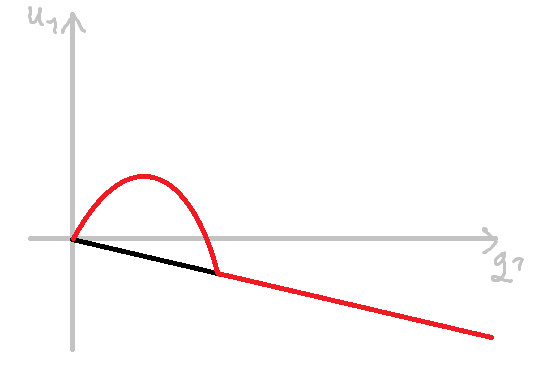
\includegraphics[scale=0.8]{graf1.png}
  \end{center}
  Tako imamo 
  $$B_1 (q_2) = \begin{cases}
    \frac{P_{max} - c - q_2}{2}; & P_{max} - c - q_2 > 0\\  
    0; & \mathrm{sicer}
  \end{cases}$$
  in simetrično 
  $$B_2 (q_1) = \begin{cases}
    \frac{P_{max} - c - q_1}{2}; & P_{max} - c - q_1 > 0\\  
    0; & \mathrm{sicer}
  \end{cases}.$$
  Od tod dobimo sistem rešitev 
  $$q_1^* = \frac{P_{max} - c - q_2^*}{2},\quad q_2^* = \frac{P_{max} - c - q_1^*}{2},$$
  ki pa je simetričen, zato zadostuje, če rešimo enačbo $q_1^* = \frac{P_{max} - c - q_1^*}{2}$.
  Od tod dobimo $(q_1^*, q_2^*) = (\frac{P_{max} - c}{3}, \frac{P_{max} - c}{3})$. Sedaj lahko naredimo primerjavo s primerom monopola.
  $$
    \begin{tabular}{c|c|c}
      & $n = 1$ & $n = 2$\\
      \hline
      \textrm{Skupna proizvodnja} & $\frac{1}{2} (P_{max} - c)$ & $\frac{2}{3} (P_{max} - c)$\\
      \hline
      \textrm{Cena produkta} & $\frac{1}{2} (P_{max} + c) $& $\frac{1}{3} (P_{max} + 2c)$\\
      \hline
      \textrm{Dobiček ene firme} & $\frac{1}{4} (P_{max} - c)^2$ & $\frac{1}{4} (P_{max} - c)^2$\\
      \hline
      \textrm{Skupni dobiček firm} & $\frac{1}{3} (P_{max} - c)^2$ & $\frac{2}{9} (P_{max} - c)^2$
    \end{tabular}    
  $$
\end{zgled}

\begin{opomba}
  Dobljeno Nashevo ravnovesje je hkrati tudi strogo Nashevo ravnovesje.
\end{opomba}

\subsection{Bertrandov model duopola}

Pri Cournotovem modelu je bila cena odvisna od proizvodnje (oziroma ekvivalentno povpraševanja).
Pri Bertrandovem modelu pa je obratno: povpraševanje je odvisno od cene.
Firme $(1, 2, \dots, n)$ izberejo ceno $p_i$ njihovega produkta, trg pa kupuje le od firme z najnižjo ceno $p = \min \{p_1, \dots, p_n\}$.
Povpraševanje trga je funkcija 
$$Q(p) = \begin{cases}
  Q_{max} - p; & p < Q_{max}\\
  0; & \textrm{sicer}
\end{cases} = (Q_{max} - p)_+.$$
Naj bo $c$ strošek proizvodnje na enoto. Povpraševanje se razdeli enakomerno med vse firme, ki imajo najnižjo ceno.
Označimo s $K(p_1, \dots, p_i)$ število firm, ki imajo najnižjo ceno.
Funkcija dobička je tako 
$$
  u_i (p_1, \dots, p_n) = \begin{cases}
    \frac{1}{K(p_1, \dots, p_n)} Q(p_i) (p_i - c); & p_i = \min \{p_1, \dots, p_n\}\\
    0; & \textrm{sicer}
  \end{cases}. 
$$
Da bo naš model sploh smiseln, moramo predpostaviti $Q_{max} > c > 0$ in $p \in [c, Q_{max}]$.
\begin{zgled}
  Oglejmo si primer duopola $n = 2$. Potem imamo 
  $$u_i (p_1, p_2) = \begin{cases}
    (Q_{max} - p_i)_+ (p_i - c); & p_i < p_j\\
    \frac{1}{2} (Q_{max} - p)_+ (p_i - c); & p_i = p_j\\
    0; & \textrm{sicer}
  \end{cases}.$$
  Ta funkcija v splošnem ni zvezna, ima pa obliko parabole.
  $$B_i(p_j) = \begin{cases}
    [c, Q_{max}]; & {p_j = c}\\
    \emptyset; & \frac{Q_{max} + c}{2} \geq p_j > c\\
    \frac{Q_{max} + c}{2}; & Q_{max} \geq p_j > \frac{Q_{max} + c}{2}
  \end{cases}.$$
  Edino Nashevo ravnovesje je $(c, c)$, ki seveda ni strogo Nashevo ravnovesje. V tem primeru nobena firma 
  ne ustvarja dobička. Enak rezultat dobimo tudi v primeru več igralcev. V Bertrandovem modelu je torej res velika razlika med monopolom in 
  ostalimi primeri.
\end{zgled}

\subsection{Vickreyeva dražba}

Imamo objekt in $n$ igralcev, kjer vsak igralec $i \in [n]$ napiše ponudbo (bid) $b_i \geq 0$ v zaprto kuverto.
Zmagovalec je tisti, ki je ponudil največjo ceno. Če dva ali več igralcev ponudi isto ceno, zmaga tisti z najnižjim 
indeksom. Zmagovalec plača za objekt drugo najvišjo ponudbo. Temu pravimo second prize sealed offers.
Vpeljemo naslednjo notacijo: naj bo $z \in [n]$ zmagovalec in cena zmagovalca
$$p(b_1, \dots, b_n) = \max \{b_i\ |\ i \in [n] \setminus \{z\}\}.$$
Vsak igralec ima vrednost $v_i$ za objekt. Funkcije preferenc so 
$$u_i (b_1, \dots, b_n) = \begin{cases}
  0; & i \neq z\\
  v_i - p(b_1, \dots, b_n); & i = z
\end{cases}.$$
Utemeljili bomo, da za igralca $i$ akcija $b_i = v_i$ dominira vse ostale akcije:
$$u_i (b_1, \dots, b_n | v_i) \geq u_i (b_1, \dots, b_n | c_i), \forall c_i.$$
Eden izmed Nashevih ravnovesij tega modela je prav profil $(v_1, v_2, \dots, v_n)$.
Oglejmo si pogoje za Nashevo ravnovesje.
\begin{itemize}
  \item Naj bo $z \in [n]$ indeks zmagovalca. Potem imamo 
  $$u_z(v_1, \dots, v_n) = v_z - p(v_1, \dots, v_n) \geq 0.$$
  Denimo, da bi $z$ spremenil svojo akcijo na $b'_z$ in še vedno zmagal. Potem je vrednost njegove funkcije preferenc še zmerom 
  $$u_z(v_1, \dots, v_n\ |\ b'_z) = v_z - p(v_1, \dots, v_n) = u_z (v_1, \dots, v_n).$$
  Če pa bi spremenil akcijo na $b'_z$ in ne bi zmagal, pa bi bilo $u_z = 0$.
  \item Za poljubnega igralca $i \neq z$ je $u_i(v_1, \dots, v_n) = 0$.
  Če spremeni svojo akcijo na $b'_i$ in ne zmaga, se nič ne spremeni.
  Če pa spremeni na $b'_i$ in zmaga, potem je 
  $$u_i (v_1, \dots, v_n\ |\ b_i') = v_i - v_z \leq 0,$$
  torej se poljubnemu igralcu ne splača zamenjati akcije.
\end{itemize}
Obstajajo tudi druga Nasheva ravnovesja, recimo če zmagovalec plača $b_z = v_z$,
vsi ostali igralci pa $b_i = 0$. Za bolj podrobno analizo igre bi predpostavili 
$v_1 \geq v_2 \geq \dots \geq v_n$. S tem sicer igro nekoliko spremenimo, saj permutiramo igralce,
igralci z nižjimi indeksi pa imajo najvišjo prioriteto.
Dražbe so zelo pomembne v praksi, pri čemer nas pogosto zanima tudi načrtovanje dražbe, ki ima želene lastnosti.
To vodi v področje, imenovano reverse game theory oziroma mechanism design.

\section{Strateške igre s funkcijami koristnosti}

Motivacija za naslednji razdelek je ta, da imajo nekatere igre kvantitativni pomen oziroma enote.
Pri takih igrah lahko naključnost uporabimo v strategiji, tako kot pri ujemanju kovancev, kjer nimamo Nashevega ravnovesja.
Osnovni princip je, da vsak igralec hoče maksimizirati $\mathbb{E} [\text{dobiček}]$.
Naj bo $A = \{a_1, a_2, \dots, a_n\}$ končna množica. Loterija na $A$ je funkcija verjetnosti na $A$, torej recimo 
$$\pi = \begin{pmatrix}
  a_1 & a_2 & \dots & a_n\\
  \pi (a_1) & \pi (a_2) & \dots & \pi (a_n)
\end{pmatrix},$$
kjer je $\sum \pi (a_i) = 1$. Nato označimo s $\Pi (A) = \Delta(A)$ množico loterij na $A$.
Če je $|A| = n$, potem je $$\Pi(A) \equiv \{(x_1, \dots, x_n) \in \R^n\ |\ x_1 + \dots + x_n = 1, x_i \geq 0,\ \forall i \in [n]\}.$$
$(n - 1)$-dimenzionalni simpleks.

\begin{opomba}
  To je konveksni prostor, saj je presek konveksnih prostorov.
\end{opomba}

\begin{definicija}
  Funkcija koristnosti na $A$ je preslikava $u: A \to \R$.
  Funkcija koristnsti $u: A \to \R$ indukcira funkcijo preferenc $\hat{u} : \Pi(A) \to \R$
  s predpisom $(\pi(a))_{a \in A} \mapsto \sum_{a \in A} u(a) \cdot \pi (a)$.
\end{definicija}

\begin{zgled}
  Naj bo $A = \{\mathrm{LJU}, \mathrm{PAR}, \mathrm{NYC}\}$ in funkcija koristnosti 
  $u: A \to \R$, ki predpiše vrednosti
  $$\mathrm{LJU} \mapsto 10,\ \mathrm{PAR} \mapsto 6,\ \mathrm{NYC} \mapsto 2.$$
  Potem je recimo 
  $$\hat{u} \begin{pmatrix}
    \mathrm{LJU} & \mathrm{PAR} & \mathrm{NYC}\\
    0.5 & 0.2 & 0.3
  \end{pmatrix} = 10 \cdot 0.5 + 6 \cdot 0.2 + 2 \cdot  0.5$$
\end{zgled}

\begin{definicija}
  Igra s funkcijami koristnosti je trojica $\Gamma = (N, (A_i)_{i \in N}, (u_i)_{i \in N})$,
  pri čemer je:
  \begin{itemize}
    \item $N$ je množica igralcev in velja $N \neq \emptyset$.
    \item $A_i$ je množica akcij za igralca $i$, kjer je $A_i \neq \emptyset$.
    \item $A = \prod_{i \in N} A_i$ je množica profilov akcij.
    \item $u_i: A \to \R$ je funkcija koristnosti za igralca $i$.
  \end{itemize}
  Množica startegij za igralca $i$ je $S_i = \Pi (A_i)$.
  Torej igralec izbere eno funkcijo verjetnosti na $A_i$.
  Množica profilov strategij je $S = \prod_{i \in N} S_i$, kjer so elementi $\pi \in S$ oblike $\pi = (\pi_i)_{i \in N}$.
  Sedaj definiramo preslikavo $U_i: S \to \R$ s predpisom 
  $$\pi = (\pi_j)_{j \in N} \mapsto \sum_{(a_j)_{j \in N} \in A} \left(\prod_{j \in N} \pi_j (a_j)\right) u_i ((a_j)_{j \in N}).$$
\end{definicija}

\begin{zgled}
  Oglejmo si primer za $n = 2$. Potem imamo 
  $$$$
  \begin{align*}
    U_1 (\pi_1, \pi_2) &= \sum_{(a_1, a_2) \in A_1 \times A_2} \left( \pi_1 (a_1) \pi_2 (a_2)\right) u_1 (a_1, a_2)\\
    &=\sum_{a_1 \in A_1} \pi_1 (a_1) \left(\sum_{a_2 \in A_2} \pi_2 (a_2) u_1 (a_1, a_2)\right)\\
    &= \sum_{a_1 \in A_1} \pi_1 (a_1) U_2 (\pi_1, \pi_2\ \big|\ \delta(a_1)), 
  \end{align*}
  kjer je $$\delta(a_1) (a_2) = \begin{cases}
    1; & a_1 = a_2\\
    0;& \textrm{sicer}
  \end{cases}.$$
\end{zgled}

Za vsako akcijo $a_i \in A_i$ obstaja čista strategija $\delta(a_i)$, definirana kot 
$$\left(\delta(a_i)\right) (a_j) = \begin{cases}
  1; & a_i = a_j\\
  0; & \textrm{sicer}
\end{cases}.$$
Nasprotje od čistih strategij so mešane. Sedaj velja 
\begin{align*}
  U_i (\pi) &= \sum_{a_i \in A_i} \pi_i (a_i) U_i(\pi\ \big|\ \delta (a_i))\\
  &= \sum_{a_i \in A_i} \pi_i (a_i) \left(\sum_{(a_j)_{j \in N\setminus \{i\}}} \left(\prod_{j \in N \setminus \{i\}} \pi_j (a_j)\right) u_i((a_j)_{j \in N})\right).
\end{align*}
Za prvega igralca imamo recimo
$$U_1 (\pi_1, \dots, \pi_n) = \sum_{a_1 \in A_1} \pi_1 (a_1) \left(\sum_{(a_2, \cdots, a_n) \in A_2 \times \dots \times A_n} \pi_2 (a_2) \dots \pi_n (a_n) u_1 (a_1, a_2, \dots, a_n)\right).$$
\begin{definicija}
  Naj bo $(N, (A_i)_{i \in N}, (u_i)_{i \in N})$ igra s funkcijami koristnosti, 
  $S = \Pi (A_i)$ in $S = \prod_{i \in N} S_i$.
  Profil strategij $\pi^* = (\pi^* _i)_{i \in N}$ je Nashevo ravnovesje natanko tedaj,
  ko velja 
  $$\forall i \in N:\ \forall \pi_i \in S_i:\ U_i (\pi^*) \geq U_i (\pi^*\ |\ \pi_i).$$
  Podobno definiramo tudi stroga Nasheva ravnovesja.
\end{definicija}

Izbira strategije za igralca $i$ je ekvivalentna ene točke v prostoru $S_i \in \Pi(A_i)$.
Torej imamo preslikavo $\Phi_{\text{kor $\to$ pref}}$ iz množice iger s funkcijami koristnosti v igre s funkcijami preferenc s predpisom 
$$(N, (A_i)_{i \in N}, (u_i)_{i \in N}) \mapsto (N, (S_i)_{i \in N}, (U_i)_{i \in N}).$$
Rečemo, da je $\Phi_{\text{kor $\to$ pref}} (\Gamma)$ mešana razširitev igre $\Gamma$.

\begin{trditev}
  Profil strategij $\pi^*$ v strateški igri $\Gamma$ je Nashevo ravnovesje natanko tedaj,
  ko je Nashevo ravnovesje v mešani razširitvi $\Phi_{\text{kor $\to$ pref}} (\Gamma)$.
\end{trditev}

\begin{zgled}
  Opazujmo naslednjo igro s funkcijami koristnosti.
  $$
  \begin{tabular}{c|c|c|}
    & \textrm{L} & \textrm{D}\\
    \hline
    \textrm{G} & 4, 2 & 2, 4\\
    \hline
    \textrm{D} & 1, 3 & 3, 2\\
    \hline
  \end{tabular}
  $$
  Sedaj definiramo množici 
  $$S_1 = \left\lbrace \begin{pmatrix}
    G & D\\
    p & 1 - p
  \end{pmatrix}\ \big|\ p \in [0, 1]\right\rbrace$$
  in 
  $$S_2 = \left\lbrace \begin{pmatrix}
    L & D\\
    q & 1 - q
  \end{pmatrix}\ \big|\ q \in [0, 1]\right\rbrace.$$
  Množico profilov strategij označimo s $S = S_1 \times S_2$ in imamo torej igro 
  $\Gamma = ([2], \left(\{G, D\}, \{L, D\} \right), (u_1, u_2))$.
  Njena mešana razširitev je $\Phi (\Gamma) = \left([2], (S_1, S_2), (U_1, U_2)\right)$,
  kjer je 
  $$U_1 (p, q) = 4pq + 2 p(1 - q) + (1 - p)q + 3 (1 - p) (1 - q)$$ 
  in za drugega igralca 
  $$U_2 (p, q) = 2pq + 4 p(1 - q) + 3 (1 - p) q + 2 (1 - p) (1 - q).$$
  Sedaj lahko najdemo Nashevo ravnovesje te nove igres pomočjo najboljših odgovorov.
  Če hočemo dobiti $B_1 (q)$, moramo poiskati odvod 
  $$\frac{\partial U_1}{\partial p} = 4q + 2 (1 - q) - q - 3(1 - q) = 1 - 4q.$$
  Sedaj imamo 
  $$B_1 (q) = \begin{cases}
    0; & 0 \leq q < \frac{1}{4}\\
    [0, 1]; & q = \frac{1}{4}\\
    1;& \frac{1}{4} < q \leq 1.
  \end{cases}.$$
  Podobno dobimo tudi za drugega igralca, in sicer 
  $$B_2 (p) = \begin{cases}
    0; & 0 \leq p < \frac{1}{3}\\
    [0, 1]; & q = \frac{1}{3}\\
    1;& \frac{1}{3} < q \leq 1.
  \end{cases}.$$
  Edino Nashevo ravnovesje je $\left(p = \frac{1}{3}, q = \frac{1}{4}\right)$.
\end{zgled}

\begin{zgled}
  Oglejmo si naslednjo igro s funkcijami koristnosti.
  $$
  \begin{tabular}{c|c|c|}
    & \textrm{A} & \textrm{B}\\
    \hline
    \textrm{X} & 3, 8 & 5, 7\\
    \hline
    \textrm{Y} & 4, 6 & 3, 6\\
    \hline
  \end{tabular}
  $$
  Potem imamo funkciji 
  $$U_1 (p, q) = 3pq + 5p(1 - q) + 4 (1 - p)q + 3(1 - p)(1 - q)$$
  in $$U_2 (p, q) = q(3p + 6(1 - p)) + (1 - q) (7p + 6 (1 - p)).$$
  Če obe funkciji odvajamo, dobimo $\frac{\partial U_1}{\partial q} = 2 - 3q$
  in $\frac{\partial U_2}{\partial p} = p.$
  Potem imamo 
  $$B_1 (q) = \begin{cases}
    1; & 0 \leq q < \frac{2}{3}\\
    [0, 1]; & q = \frac{2}{3}\\
    0; & \frac{2}{3} < q \leq 1
  \end{cases}$$
  in $$B_2 (p) = \begin{cases}
    [0, 1]; & p = 0\\
    1; & 0< p < 1
  \end{cases}.$$
  Ta igra je degenerirana.
  Iz skice je razvidno, da so Nasheva ravnovesja oblike $\left(p = 0, \frac{2}{3} \leq q \leq 1\right)$.
\end{zgled}

\begin{definicija}
  Igra za dva igralca je degenerirana, če ima eden izmed igralcev mešano strategijo, ki 
  določi pozitivno verjetnost natanko $k$-tim čistim strategijam,
  tako da ima drugi igralec strogo več kot $k$ čistih najboljših odgovorov na to strategijo.
\end{definicija}

\subsection{Obstoj mešanih Nashevih ravnovesij}

\begin{izrek}[Nash, 1949]
  Vsaka strateška igra s funkcijami koristnosti, kjer ima vsak igralec končno množico akcij,
  ima vsaj eno Nashevo ravnovesje.
\end{izrek}

\begin{opomba}
  Dokaz je nekonstruktiven, saj nam pokaže le eksistenco Nashevega ravnovesja, ne pa tudi, kako ga najti.
\end{opomba}

\begin{opomba}
  Če je igra generična (oziroma nedegenerirana), je število Nashevih ravnovesij liho.
\end{opomba}

\begin{trditev}[Sistem neenačb]
  Profil strategij $\pi^* = (\pi^* _i)_{i \in N}$ je Nashevo ravnovesje natanko tedaj, ko velja 
  \begin{equation*}
    \forall i \in N:\ \forall a_i \in A_i:\ U_i (\pi^*) \geq U_i (\pi^*\ |\ \delta (a_i)). \label{eq:1}
  \end{equation*}
\end{trditev}

\begin{dokaz}
  Trditev $(\Rightarrow)$ je trivialna.
  Dokažimo torej $(\Leftarrow)$. Naj bo $\pi^*$ profil strategij, za katero velja predpostavka \ref{eq:1}.
  Fiksiramo $i \in N$ ter $\pi_i \in S_i$. Potem je 
  \begin{align*}
    U(\pi^*\ |\ \pi_i) &= \sum_{a_i \in A_i} \pi (a_i) U_i (\pi^*\ |\ \delta(a_i))\\
    &= \sum_{a_i \in A_i} \pi_i (a_i) U_i (\pi^*)\\
    &= U(\pi^*) \sum_{a_i \in A_i} \pi_i(a_i) = U(\pi^*). \qedhere
  \end{align*}
\end{dokaz}

Za preverjanje, ali je kandidat $\pi^*$ Nashevo ravnovesje, moramo preveriti le spremembe na vse čiste akcije.

\begin{zgled}
  Oglejmo si spet igro iz prejšnjega zgleda.
  $$
  \begin{tabular}{c|c|c|}
    & \textrm{L} & \textrm{D}\\
    \hline
    \textrm{G} & 4, 2 & 2, 4\\
    \hline
    \textrm{D} & 1, 3 & 3, 2\\
    \hline
  \end{tabular}
  $$
  Po definiciji je $(p^*, q^*)$ Nashevo ravnovesje natanko tedaj, ko je 
  $$\forall p \in [0, 1]:\ U_1 (p^*, q^*) \geq U_1 (p, q^*)$$
  in $$\forall q \in [0, 1]:\ U_2 (p^*, q^*) \geq U_2 (p^*, q).$$
  Iz trditve pa dobimo, da je $(p^*, q^*)$ Nashevo ravnovesje natanko tedaj, ko je 
  $$U_1 (p^*, q^*) \geq U_1 (0, q^*),\quad U_1 (p^*, q^*) \geq U_1 (1, q^*)$$ in 
  $$U_2 (p^*, q^*) \geq U_2 (p^*, 0),\quad U_2 (p^*, q^*) \geq U_2 (p^*, 1).$$
  Tako smo sedaj iz neskončne družine neenačb dobili le končno število neenačb.
\end{zgled}

\begin{trditev}[Princip indiferentnosti]
  Če je profil strategij $\pi^* = (\pi_i)_{i \in N}$ Nashevo ravnovesje, potem velja 
  $$\forall i \in N:\ \forall a_i \in A_i:\ \left(\pi_i^* (a_i) > 0 \Rightarrow U_i (\pi^*\ |\ \delta(a_i)) = U_i(\pi^*)\right)$$
\end{trditev}

\begin{dokaz}
  Dokažimo s protislovjem, torej predpostavimo, da je $\pi^*$ Nashevo ravnovesje in sklep ne drži.
  Obstajata torej taka $i \in N$ in $b_i \in A_i$, za katera velja $\pi^*_i (b_i) > 0$ 
  in $U_i (\pi^*) \neq U_i (\pi^*\ |\ \delta(b_i))$. 
  ker je $\pi^*$ Nashevo ravnovesje, po sistemu neenačb velja 
  $$\forall a_i \in A_i:\ U_i (\pi^*) \geq U_i (\pi^*\ |\ \delta(a_i)).$$
  Iz tega dobimo $U_i (\pi^*) > U_i (\pi^*\ |\ \delta(b_i))$.
  Sedaj poračunamo:
  \begin{align*}
    U_i (\pi^*) &= \sum_{a_i \in A_i} \pi^*_i (a_i) U_i (\pi^*\ |\ \delta(a_i))\\
    &= \pi^*_i (b_i) U_i (\pi^*\ |\ \delta(b_i)) + \sum_{a_i \in A_i \setminus \{b_i\}}\pi^*_i (a_i) U_i (\pi^*\ |\ \delta(a_i))\\
    &> \pi^*_i (b_i) U(\pi^*) + \sum_{a_i \in A_i \setminus \{b_i\}}\pi^*_i (a_i) U_i (\pi^*)\\
    &= U_i (\pi^*) \sum_{a_i \in A_i} \pi_i ^* (a_i) = U_i (\pi^*).
  \end{align*}
  Torej smo dobili $U_i (\pi^*) > U_i (\pi^*)$, protislovje.
\end{dokaz}

Princip indiferentnosti uporabimo za iskanje kandidatov za Nashevo ravnovesje, nato pa uporabimo 
sistem neenačb, da kandidate res preverimo. Poseben primer je, ko je $A_i = \{a_i, b_i\}$ za vsak $1 = 1, \dots, n$.
Potem je $\pi^*$ Nashevo ravnovesje, pri čemer vsak igralec meša, natanko tedaj, ko velja 
$$\forall i \in N:\ U_i (\pi^*\ |\ \delta(a_i)) = U_i (\pi^*\ |\ \delta(b_i)).$$

\begin{zgled}
  Vrnimo se k igri 
  $$
  \begin{tabular}{c|c|c|}
    & \textrm{L} & \textrm{D}\\
    \hline
    \textrm{G} & 4, 2 & 2, 4\\
    \hline
    \textrm{D} & 1, 3 & 3, 2\\
    \hline
  \end{tabular}
  $$
  in predpostavimo 
  $$\Pi_1 (p) = \begin{pmatrix}
    G & D\\
    p & 1 - p
  \end{pmatrix}, \quad \Pi_2 (q) = \begin{pmatrix}
    L & D\\
    q & 1 - q
  \end{pmatrix}.$$
  Obravnavajmo primer $p = 0$; tedaj prvi igralec izbere strategijo $\delta(D)$.
  Potem imamo najboljši odgovor $B_2 (\delta(D)) = \delta(L)$
  in nato $B_1 (\delta(L)) = \delta(G) \neq \delta(D)$, torej ne obstaja Nashevo ravnovesje s $p = 0$.
  Na enak način preverimo, da ne obstaja Nashevo ravnovesje s $p = 1$.
  S tem dobimo enačbo za kandidata za Nashevo ravnovesje 
  $$4q + 2(1 - q) = q + 3(1 - q),$$
  od koder dobimo $q = \frac{1}{4}$.
  Sedaj moramo preveriti še s sistemom neenačb:
  $$\frac{1}{4} (2p + 3(1 - p)) + \frac{3}{4} (4p + 2(1 - p)) \geq (2p + 3(1 - p))$$
  in 
  $$\frac{1}{4} (2p + 3(1 - p)) + \frac{3}{4} (4p + 2(1 - p)) \geq (4p + 2(1 - p)).$$
  Ti dve enačbi se poenostavita v $$4p + 2(1 - p) = 2p + 3(1 - p),$$
  zato res dobimo $p = \frac{1}{3}.$
\end{zgled}

\begin{zgled}
  Oglejmo si ponovno igro 
  $$
  \begin{tabular}{c|c|c|}
    & \textrm{A} & \textrm{B}\\
    \hline
    \textrm{X} & 3, 8 & 5, 7\\
    \hline
    \textrm{Y} & 4, 6 & 3, 6\\
    \hline
  \end{tabular}
  $$
  in vzemimo 
  $$\Pi_1 (p) = \begin{pmatrix}
    X & Y\\
    p & 1 - p
  \end{pmatrix}, \quad \Pi_2 (q) = \begin{pmatrix}
    A & B\\
    q & 1 - q
  \end{pmatrix}.$$
    Vzemimo $p = 0$: potem prvi igralec uporabi $\delta(Y)$.
  Potem je $$B_2 (\delta(Y)) = \left\lbrace \begin{pmatrix}
    A & B\\
    q & 1 - q
  \end{pmatrix}\ \Big|\ q \in [0, 1] \right\rbrace.$$
  Poiskati moramo, kdaj je $$B_1 \left(\begin{pmatrix}
    A & B\\
    q & 1 - q
  \end{pmatrix}\right) = \delta(Y).$$
  Po sistemu neenačb se to zgodi natanko tedaj, ko je 
  $$U_1 (\delta(Y), q) \geq U_1(\delta(X), q),$$
  kar pa je ekvivalentno 
  $$4q + 3 (1 - q) \geq 3q + 5 (1 - q).$$
  Od tod dobimo $q \geq \frac{2}{3}$.
  S tem smo dobili Nashevo ravnovesje $(\delta(Y), q)$ za $q \in \left[\frac{2}{3}, 1\right]$.
  V primeru $p = 1$ podobno kot v prejšnjem zgledu preverimo, da to ni Nashevo ravnovesje.
  Preostane nam le še $p \in (0, 1)$: zaradi principa indiferentnosti za prvega igralca velja
  $U_1 (0, q) = U_1(1, q)$ in od tod 
  $$3q + 5(1 - q) = 4 q + 3 (1 - q).$$
  S tem dobimo $q = \frac{2}{3}$ in iz principa indiferentnosti dobimo kandidat za Nashevo ravnovesje: 
  $$8p + 6(1 - p) = 7p + 6(1 - p),$$
  pri čemer dobimo $p = 0$, kar je protislovje. Torej v primeru 
  $p \in (0, 1)$ ne dobimo nobenih novih Nashevih ravnovesij. 
\end{zgled}

\begin{definicija}
  Naj bo igra s funkcijami koristnosti $(N, (A_i)_{i \in N}, (u_i)_{i \in N})$, označimo strategije $S_i = \Pi(A_i)$ in množico profilov strategij
   $S = \prod_{i \in N} S_i$.
   Strategija $\alpha_i \in S_i$ šibko dominira $\beta_i \in S_i$, če velja 
   $$\forall \pi \in S:\ U_i (\pi\ |\ \alpha_i) \geq U_i (\pi\ |\ \beta_i).$$
   Če je v zgornji neeenačbi strogi neenačaj, rečemo, da $\alpha_i$ 
   strogo dominira $\beta_i$. 
\end{definicija}

\begin{trditev}
  Naj bo $\pi^* = (\pi_i^*)_{i \in N}$ Nashevo ravnovesje.
  Če strategija $\alpha_i \in S_i$ strogo dominira neko čisto strategijo 
  $\delta(b_i) \in S_i$, potem $\pi_i^* (b_i) = 0.$
\end{trditev}

\begin{dokaz}
  Ker $\alpha_i$ strogo dominira $\delta(b_i)$, velja 
  $$U_i (\pi^*\ |\ \alpha_i) > U_i (\pi^*\ |\ \delta(b_i)).$$
  Predpostavimo nasprotno, da je $\pi_i^* (b_i) \neq 0$, torej $\pi_i^* (b_i) > 0$.
  Definiramo novo strategijo za igralca $i$
  $$\widetilde{\pi}_i (a_i) = \begin{cases}
    \alpha_i (b_i) \pi_i^*(b_i); & a_i = b_i\\
    \pi^* _i (a_i) + \alpha_i (a_i) \pi^*_i (b_i); & a_i \neq b_i
  \end{cases}.$$
  Preveriti moramo, da je $\widetilde{\pi}_i $ res strategija, torej da je $\widetilde{\pi}_i (a_i) \geq 0$ za vsak $a_i \in A_i$ in 
  $\sum_{a_i \in A_i} \widetilde{\pi}_i (a_i) = 1.$
  Poračunamo:
  \begin{align*}
    &\alpha(b_i) \pi_i^* (b_i) + \sum_{a_i \in A_i \setminus \{b_i\}} \left(\pi_i^* (a_i) + \alpha_i (a_i) \pi_i^* (b_i)\right)\\
    &= \sum_{a_i \in A_i \setminus \{b_i\}} \pi_i^* (a_i) + \sum_{a_i \in A_i} \alpha_i (a_i) \pi_i^* (b_i)\\
    &= \sum_{a_i \in A_i \setminus \{b_i\}} \pi_i^* (a_i) + \pi_i^* (b_i) = 1.
  \end{align*} 
  Sedaj imamo:
  \begin{align*}
    U_i (\pi^*\ |\ \widetilde{\pi}_i) &= \sum_{a_i \in A_i} \widetilde{\pi}_i (a_i) \cdot U_i (\pi^*\ |\ \delta(a_i))\\
    &= \widetilde{\pi}_i (b_i) U_i (\pi^*\ |\ \delta(b_i)) + \sum_{a_i \in A_i \setminus \{b_i\}} \widetilde{\pi}_i (a_i) U_i (\pi^*\ |\ \delta (a_i))\\
    &= \alpha_i (b_i) \pi_i ^* (b_i) U_i (\pi^*\ |\ \delta(b_i)) + \sum_{a_i \in A_i \setminus \{b_i\}} (\pi_i ^* (a_i) + \alpha_i(a_i) \pi_i^*(b_i)) U_i (\pi^*\ |\ \delta (a_i))\\
    &= \left( \sum_{a_i \in A_i} \alpha_i (a_i) U_i (\pi_i ^*\ |\ \delta(a_i)) \right) \cdot \pi_i^* (b_i) + \sum_{a_i \in A_i \setminus \{b_i\}} \pi_i^* (a_i) U_i (\pi^*\ |\ \delta(a_i))\\
    &= U_i (\pi^*\ |\ \alpha_i) \cdot \pi_i ^* (b_i) + \sum_{a_i \in A_i \setminus \{b_i\}} \pi_i^* (a_i) U_i (\pi^*\ |\ \delta(a_i))\\
    &> U_i (\pi^*\ |\ \delta(b_i)) \pi_i ^* (b_i) + \sum_{a_i \in A_i \setminus \{b_i\}} \pi_i^* (a_i) U_i (\pi^*\ |\ \delta(a_i))\\
    &= \sum_{a_i \in A_i} \pi_i^* (a_i) U_i (\pi^*\ |\ \delta(a_i)) = U_i (\pi^*). \qedhere
  \end{align*}
\end{dokaz}

\begin{opomba}
  Pri iskanju enega Nashevega ravnovesja, lahko odstranimo šibko dominirane strategije.
\end{opomba}

\begin{dokaz}[Dokaz Nashevega ravnovesja]
  Na začetku uporabimo nekaj lastnosti konveksne množice $X \subseteq \R^d$.
  Vemo, da če sta $X, Y$ konveksni, potem sta tudi množici $X \times Y$ in $X \cap Y$ konveksni.
  Od tod vidimo, da je množica 
  $$S_i (A) = \Pi(A_i) = \{(\pi_i(a_i))_{a_i \in A_i}\ |\ \sum_{a_i \in A_i} \pi_i (a_i) = 1,\ \pi_i (a_i) \geq 0,\ \forall a_i \in A_i\}.$$
  konveksna, torej je tudi $S = \prod_{i \in N} S_i$ konveksna. 
  Očitno je tudi, da je $S_i$ kompaktna, saj je zaprta in omejena, torej je tudi $S$ kompaktna.
  Sedaj uporabimo Brouwerjev izrek o negibni točki: če je $X \subseteq \R^d$
  konveksna in kompaktna in $T: X \to X$ zvezna preslikava, 
  potem ima $T$ negibno točko.
  Sedaj definiramo preslikavo 
  $T: S \to S$ s predpisom 
  $\pi = (\pi_i)_{i \in N} \mapsto (\widetilde{\pi}_i)_{i\in N} = \widetilde{\pi}$,
  kjer je 
  $$\widetilde{\pi}_i (a_i) = \frac{\pi_i (a_i) + \max \{0, U_i (\pi\ |\ \delta(a_i)) - U_i (\pi)\}}{1 + \sum_{b_i \in A_i} \max \{0, U_i (\pi\ |\ \delta(b_i)) - U_i (\pi)\}}.$$
  Najprej moramo preveriti, da je $\widetilde{\pi}$ res strategija.
  Očitno velja $\widetilde{\pi}_i (a_i) \geq 0$ za vsak $i \in N$ ter $a_i \in A_i$.
  Hitro pa lahko preverimo tudi, da velja $\sum_{a_i \in A_i} \widetilde{\pi}_i (a_i) = 1$ za vsak $i \in N$.
  Torej je $T$ res preslikava v $S$ in je celo kompozitum zveznih preslikav, torej je zvezna.
  Ker je množica $S$ kompaktna in konveksna, ima $T$ negibno točko $\pi^* \in S$, torej velja 
  $T(\pi^*) = \pi^*$. Dokazali bomo, da je to Nashevo ravnovesje.
  Ker je 
  $$U_i (\pi^*) = \sum_{a_i \in A_i} \pi_i^* U_i (\pi^*\ |\ \delta(a_i)),$$
  obstaja $c_i \in A_i$ z $\pi_i^* (c_i) > 0$ in $U_i (\pi^*) \geq U_i (\pi^*\ |\ \delta(c_i))$.
  Sedaj fiksiramo $i \in N$. Za ta $c_i \in A_i$ imamo 
  \begin{align*}
    \pi_i ^* (c_i) &= \frac{\pi_i^* (c_i) + \max \{0, U_i (\pi^*\ |\ \delta(c_i)) - U_i (\pi^*)\}}{1 + \sum_{b_i \in A_i} \max \{0, U_i (\pi^*\ |\ \delta(b_i)) - U_i (\pi^*)\}}\\ 
    &= \frac{\pi_i^* (c_i)}{1 + \sum_{b_i \in A_i} \max \{0, U_i (\pi^*\ |\ \delta(b_i)) - U_i (\pi^*)\}} > 0,
  \end{align*}
  torej je $\sum_{b_i \in A_i} \max \{0, U_i (\pi^*\ |\ \delta(b_i)) - U_i (\pi^*)\} = 0.$
  Od tod sledi, da za vsak $b_i \in A_i$ velja $U_i (\pi^*\ |\ \delta(b_i)) \leq U_i (\pi^*)$, torej 
  $$\forall i \in N:\ \forall b_i \in A_i:\ U_i (\pi^*) \geq U_i(\pi^*\ |\ \delta(b_i)),$$
  kar pa je ravno karakterizacija Nashevega ravnovesja iz sistema neenačb.
\end{dokaz}

\section{Matrične in bimatrične igre}

\subsection{Bimatrične igre}

Bimatrične igre so igre, kjer imamo dva igralca $i = 1, 2$ in 
akcije $A_1 = [m] = \{1, \dots, m\}$ in $A_2 = [n] = \{1, \dots, n\}$.
Funkcije koristnosti tako kot prej označimo z $u_i$, igro pa predstavimo z (bi)matriko 
$$\begin{bmatrix}
  A & B
\end{bmatrix} = \begin{bmatrix}
  u_1(i, j) & u_2 (i, j)
\end{bmatrix}_{i \in [m],\ j \in [n]}.$$
Funkcije preferenc podamo kot vektorje:
$$S_1 = \Pi([m]) = \left\lbrace \begin{bmatrix}
  p_1 \\ \vdots \\ p_m
\end{bmatrix}\ \Big|\ p_1, \dots, p_m \geq 0, \sum_{i \in [m]} p_i = 1 \right\rbrace$$
oziroma 
$$S_2 = \Pi([n]) = \left\lbrace \begin{bmatrix}
  q_1 \\ \vdots \\ q_n
\end{bmatrix}\ \Big|\ q_1, \dots, q_n \geq 0, \sum_{i \in [n]} q_i = 1 \right\rbrace.$$
Naj bo igra $\begin{bmatrix}
  A & B
\end{bmatrix}$, $p \in S_1$, $q \in S_2$ in $A \in \R^{n \times m}$.
Potem imamo funkcijo preferenc za prvega igralca
\begin{align*}
  U_1 (p, q) &= p^{\top} A q\\
  &= \begin{bmatrix}
    p_1 & \cdots & p_m
  \end{bmatrix} \begin{bmatrix}
    a_{11} & \cdots & a_{1n}\\
    \vdots & & \vdots\\
    a_{n1} & \cdots & a_{nn}
  \end{bmatrix} \begin{bmatrix}
    q_1 \\ \vdots \\q_n
  \end{bmatrix}\\
  &= \begin{bmatrix}
    p_1 & \cdots & p_m
  \end{bmatrix} \begin{bmatrix}
    \sum_{i = 1} ^n a_{1i} q_{i}\\
    \vdots\\
    \sum_{i = 1} ^n a_{mi} q_{i}
  \end{bmatrix}\\
  &= \sum_{i = 1} ^m p_i \left(\sum_{j = 1}^n a_{ij} q_j\right)\\
  &= \sum_{i = 1} ^m \sum_{j = 1} ^n a_{ij} p_i q_j.
\end{align*}
Podobno je za drugega igralca $U_2 (p, q) = p^\top B q$.
Takoj vidimo, da imamo tudi 
$$U_1 (\delta(i), q) = \left[Aq\right]_i = \begin{bmatrix}
  0 & \cdots & 0 & 1 & 0 & \cdots & 0
\end{bmatrix} Aq$$
in simetrično $U_2 (p, \delta(j)) = [p^\top B]$.
Sedaj lahko prevedemo Nashevo ravnovesje v novo notacijo matričnih iger.
\begin{trditev}
  Matrična igra ima Nashevo ravnovesje $(p^*, q^*)$ natanko tedaj, ko velja:
  $$\begin{cases}
    \forall p \in S_1:\ p^\top A q^* \leq (p^*)^\top A q^*\\
    \forall q \in S_2:\ (p^*)^\top B q \leq (p^*)^\top B q^*
  \end{cases}
  $$
\end{trditev}
\begin{trditev}[Sistem neenačb]
  Profil strategij $(p^*, q^*)$ je Nashevo ravnovesje natanko tedaj, ko velja:
  $$\begin{cases}
    \forall i \in [m]:\ [A q^*]_i \leq (p^*)^\top A q^*\\
    \forall j \in [n]:\ [(p^*)^\top B]_j \leq (p^*)^\top B q^*
  \end{cases}.
  $$
\end{trditev}
\begin{trditev}[Princip indiferentnosti]
  Če je profil strategij $(p^*, q^*)$ Nashevo ravnovesje, potem:
  $$\begin{cases}
    \forall i \in [m]:\ p_i^* > 0 \Rightarrow [A q^*]_i = (p^*)^\top A q^*\\
    \forall j \in [n]:\ q_j^* > 0 \Rightarrow [(p^*)^\top B]_j = (p^*)^\top B q^*
  \end{cases}.
  $$
\end{trditev}
Ta izreka nam data algoritem za iskanje Nashevih ravnovesij pri matričnih igrah.
Najprej s principom indiferentnosti poiščemo kandidate, torej za poljubni 
množici indeksov $I \subseteq [m],\ J \subseteq [n]$ iščemo rešitve sistema linearnih enačb 
    \begin{gather}
      [Aq]_i = [Aq]_{i'},\ \forall i, i' \in I \tag{$3$} \label{eq:3}\\
      q_j = 0,\ \forall j \in [n]\setminus J \nonumber\\
      \sum_{j = 1} ^n q_j = 1 \nonumber\\
      [p^\top B]_j = [p^\top B]_{j'},\ \forall j, j' \in J \nonumber\\
      p_i = 0,\ \forall i \in [m] \setminus I \nonumber\\
      \sum_{i = 1} ^n p_i = 1 \nonumber,
    \end{gather}
nato pa s sistemom neenačb preverimo,
če ustrezajo pogojem:
\begin{gather*}
  p^\top A q \geq [Aq]_i,\ \forall i \in [m] \setminus I \tag{$4$} \label{eq:4}\\
  q_j \geq 0,\ \forall j \in [n] \nonumber\\
  p^\top B q \geq [p^\top B]_j,\ \forall j \in [n]\setminus J \nonumber\\
  p_i \geq 0,\ \forall i \in [m] \nonumber.
\end{gather*} 

\begin{algorithm}
  \caption{Iskanje Nashevih ravnovesij pri bimatričnih igrah}\label{alg:nash}
  \begin{algorithmic}[1]
    \State izberi poljubno $I \subseteq [m]$
    \State izberi poljubno $J \subseteq [n]$
    \State za izbrani $I, J$ reši sistem \eqref{eq:3}
    \State če rešitev sistema \eqref{eq:3} ustreza \eqref{eq:4}, je to Nashevo ravnovesje
    %\For{$I \subseteq [m]$}
    %\For{$J \subseteq [n]$}
    %  \State reši sistem \eqref{eq:3};
    %  \If{rešitev \eqref{eq:3} ustreza \eqref{eq:4}}
    %      \State vrni rešitev;
    %  \EndIf
    %\EndFor
  %\EndFor
  \end{algorithmic}
\end{algorithm}

Za generične situacije bo obstajala rešitev natanko tedaj, ko je $|I| = |J|$.
Ta algoritem je zelo počasen, vendar pa boljšega v praksi ni.
Problem iskanja Nashevega ravnovesja v matričnih igrah je PPAD-complete.
Če ima matrična igra števila v $\Z$ oziroma $\Q$, bodo običajno imela 
Nasheva ravnovesja v $\Q$. To pa ne velja za $3$ igralce.
Obstajajo namreč igre za $3$ igralce, ki so generične, 
imajo števila v $\Z$ in imajo natanko eno Nashevo ravnovesje, 
ki je iracionalno število.

Sedaj se osredotočimo na primer, ko je $m = 2$ ali $n = 2$.
Oglejmo si primer, ko je $m = 2$, saj je drugi simetričen.
$$\begin{bmatrix}
  A & B
\end{bmatrix}
= \begin{bmatrix}
  a_{11}, b_{11} & \cdots & a_{1n}, b_{1n}\\
  a_{21}, b_{21} & \cdots & a_{2n}, b_{2n}
\end{bmatrix}.
$$
Strategije za 1. igralca so 
$$\begin{pmatrix}
  1 & 2\\
  p & 1 - p
\end{pmatrix}.$$
Sedaj lahko dobimo najboljši odgovor drugega igralca za $p \in [0, 1]$.
Imamo linearno funkcijo $$U_2 \left(\begin{bmatrix}
  p \\ 1 - p
\end{bmatrix}, \delta(j)\right) = b_{1, j} p + b_{2, j} (1 - p).$$
Zgornja ovojnica teh funkcij določi najboljši odgovor.
$$\mathrm{zgornja}(p) = \max_{j \in [n]} U_2 \left(\begin{bmatrix}
  p\\ 1 - p
\end{bmatrix}, \delta(j)\right).$$ 
Opazujemo vsak del zgornje ovojnice posebej (princip indiferentnosti).

\begin{zgled}
  Oglejmo si igro
  $$\begin{bmatrix}
    A & B
  \end{bmatrix} = 
  \begin{bmatrix}
    5, 7 & 2, 2 & 3, 4 & 2, 5\\
    2, 1 & 4, 9 & 1, 7 & 6, 2
  \end{bmatrix}.$$
  Potem iščemo najboljše odgovore:
  \begin{gather*}
    U_2 (p, \delta(1)) = 7p + 1 - p = 1 + 6p\\
    U_2 (p, \delta(2)) = 2p + 9(1 - p) = 9 - 7p\\
    U_2 (p, \delta(3)) = 4p + 7(1 - p) = 7 - 3p\\
    U_2 (p, \delta(4)) = 5p + 2(1 - p) = 2 + 3p.
  \end{gather*}
  \begin{center}
    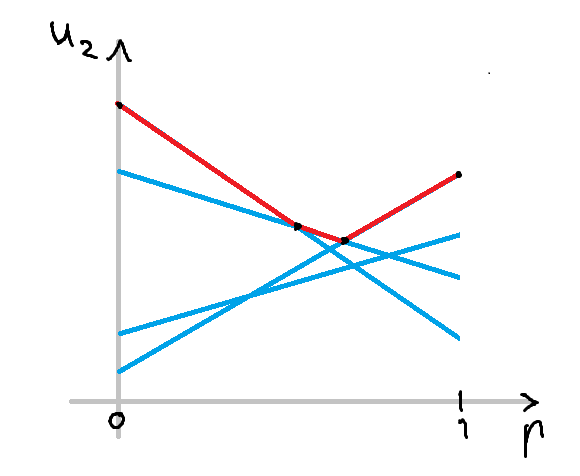
\includegraphics[scale=0.8]{graf2.png}
  \end{center}
  Presečišča premic, ki so za nas relevantna, so:
  \begin{gather*}
    1 + 6p = 9 - 7p\\
    9 - 7p = 7 - 3p\\
    1 + 6p = 7 - 3p.
  \end{gather*}
  Od tod dobimo točke $\left(\frac{1}{2}, \frac{11}{2}\right)$,
  $\left(\frac{8}{13}, \frac{61}{13}\right)$, $\left(\frac{2}{3}, 5\dots\right)$.
  Tako dobimo funkcijo najboljšega odgovora za 2. igralca:
  $$
  \begin{cases}
    \delta(2); & 0 \leq p < \frac{1}{2}\\
    \lambda \delta(2) + (1 - \lambda) \delta(3); & p = \frac{1}{2}\\
    \delta(3); & \frac{1}{2} < p < \frac{2}{3}\\
    \mu \delta(3) + (1 - \mu) \delta(1); & p = \frac{2}{3}\\
    \delta(1); & \frac{2}{3} < p \leq 1.
  \end{cases}
  $$
  V primeru $0 \leq p < \frac{1}{2}$ mora za Nashevo ravnovesje veljati $B_1(\delta(2)) \in [0, 1 / 2).$
  Res imamo $B_1(\delta(2)) = 0$, torej smo dobili prvo Nashevo ravnovesje pri $p = 0$ za prvega igralca in 
  $\delta(2)$ za drugega.
  Za primer $p = \frac{1}{2}$ uporabimo princip indiferentnosti za prvega igralca, 
  od koder dobimo 
  $$\frac{1}{2} (3 - \lambda) + \frac{1}{2} (1 + 3\lambda) = 3 - \lambda.$$
  Torej imamo kandidata za Nashevo ravnovesje pri $p = 2$ in  
  $$\begin{bmatrix}
    0\\ 1/2 \\ 1/2\\ 0
  \end{bmatrix},$$
  ki pa je res Nashevo ravnovesje, saj po konstrukciji ustreza neenakostim iz sistema neenačb.
  Primer $\frac{1}{2} < p < \frac{2}{3}$ nam ni treba obravnavati, saj bi dobili kvečjemu čisto strategijo 
  za prvega igralca.
  Oglejmo si torej $p = \frac{2}{3}$.
  Iz principa indiferentnosti za prvega igralca dobimo 
  $$\frac{2}{3} (3\mu + 2) + \frac{1}{3} (1 + \mu) = 3 \mu + 2,$$
  ki ima rešitev $\mu = - \frac{1}{2}$, torej za to ne dobimo kandidata za Nashevo ravnovesje.
  Nazadnje dobimo še Nashevo ravnovesje za $p = 1$, kjer drugi igralec izbere strategijo $\delta(1)$.
\end{zgled}

Ta procedura je učinkovita, saj ima zgornja ovojnica za $n$ linearnih funkcij največ $n$ delov.
Linearnost velja tudi v primeru $m = 3$, ne pa več v $m = 4$.

\subsection{Stopnja varnosti}

Koliko lahko vsak igralec zagotovi, ne glede na to, kar igrajo ostali igralci?
Za bimatrično igro definiramo stopnjo varnosti za prvega igralca
$$v_1 = \max_{p \in S_1} \min_{q \in S_2} p^\top A q.$$
Prvi igralec lahko torej zagotovi $v_1$ enot. Simetrično je 
stopnja varnosti za drugega igralca enaka 
$$v_2 = \max_{q \in S_2} \min_{p \in S_1} p^\top B q.$$

\begin{trditev}
  Veljata identiteti $$v_1 = \max_{p \in S_1} \min_{q \in [n]} [p^\top A]_j,\quad v_2 = \max_{q \in S_2} \min_{i \in [m]} [Bq]_j.$$
\end{trditev}

\begin{dokaz}
  Za $\forall p \in S_2$ velja $\min_{q \in S_2} p^\top A q = \min_{q \in S_2} \sum_{j \in [n]} [p^\top A]_j = \min_{j \in [n]} [p^\top A]_j$.
\end{dokaz}

\begin{definicija}
  Strategija $\widetilde{p} \in S_1$ je maxmin strategija, če velja 
  $$v_1 = \min_{q \in S_2} \widetilde{p}^\top Aq = \min_{j \in [n]} [\widetilde{p}^\top A]_j.$$
  Simetrično je $\widetilde{q} \in S_2$ maxmin strategija, če velja 
  $$v_2 = \min_{p \in S_1} p^\top B \widetilde{q} = \min_{i \in [m]} [B\widetilde{q}]_i.$$
\end{definicija}

\begin{zgled}
  Oglejmo si igro 
  $$\begin{bmatrix}
    2, 1 & 3, 4\\
    5, 2 & 1, 3
  \end{bmatrix}.$$
  Tukaj imamo stopnjo varnosti za prvega igralca
  $$v_1 = \max_{p \in [0, 1]} \min \{5 - 3p, 1 + 2p\}$$
  in dobimo $v_1 = \frac{13}{5}$ pri $p = \frac{4}{5}$.
  Podobno lahko naredimo za drugega igralca in dobimo 
  $$v_2 = \max_{q \in [0, 1]} \min \{4 - 3q, 3 - q\}.$$
  Funkcija $\min \{4 - 3q, 3 - q\}$ je padajoča, zato je želeni $q = 0$.
  Seveda bi lahko že prej opazili, da drugi stolpec dominira prvega.
\end{zgled}

\begin{trditev}
  Naj bo $p \in S_1$ maxmin strategija za prvega igralca. 
  Potem velja 
  $$\forall q \in S_2:\ p^\top A q \geq v_1.$$
\end{trditev}

\begin{dokaz}
  Če je $p$ maxmin, je $v_1 = \min_{j \in [n]} [P^\top A]_j$.
  Od tod pa naprej sledi $$\forall j \in [n]:\ [p^\top A]_j \geq v_1.$$
  Od tod pa po definiciji sledi 
  \begin{equation*}
    \forall q \in S_2:\ p^\top A q = \sum_{j \in [n]} [p^\top A]_j q_j \geq \sum_{j \in [n]} v_1 q_j = v_1. \qedhere
  \end{equation*}
\end{dokaz}

\begin{trditev}
  Množica 
  $$S_1 ^* = \{p \in S_1\ |\ \text{$p$ maxmin za prvega igralca}\}$$
  je konveksna.
\end{trditev}

\begin{dokaz}
  Naj bosta $p, p' \in S_1^*$.
  Ponovno imamo 
  $$v_1 = \min_{j \in [n]} [p^\top A]_j \Rightarrow v_1 \leq [p^\top A]_j,\ \forall j \in [n].$$
  Podobno dobimo tudi za drugo maxmin strategijo $p'$:
  $$v_1 \leq [p'^\top A]_j,\ \forall j \in [n].$$
  Za poljuben $\lambda \in [0, 1]$ definiramo $\widetilde{p} = (1 - \lambda)p + \lambda p'$ in dobimo 
  \begin{align*}
    [\widetilde{p}^\top A]_j &= [((1 - \lambda)p + \lambda p')^\top A]_j\\
    &= [((1 - \lambda)p^\top + \lambda p'^\top) A]_j\\
    &= (1 - \lambda) [p^\top A]_j + \lambda [p'^\top A]_j\\
    &\geq v_1,\ \forall j \in [n].   \qedhere
  \end{align*}
\end{dokaz}

Stopnja varnosti ni rezervirana le za bimatrične igre; prav tako jo lahko definiramo za več igralcev.
V tem primeru jo iščemo s pomočjo linearnega programiranja.

\begin{algorithm}
  \caption{LP problem}
  \begin{algorithmic}[1]
      \State maksimiziraj ali minimiziraj funkcijo: $c^\top x$
      \State pri pogojih: $Ax \leq b$ 
      \State kjer: $x \in \R^n$, fiksiramo: $A \in \R^{n \times n}, b, c \in \R^n$ 
  \end{algorithmic}
\end{algorithm}

LP problem je:
\begin{itemize}
  \item nedopusten, če za noben $x$ ne velja $Ax \leq b$.
  \item neomejen, če za vsak $u \in \R$ obstaja tak $x \in \R,\ A x \leq b$,
  da velja $c^\top x \geq u$ (iščemo minimum) ali pa $c^\top x \geq u$ (iščemo maksimum).
  \item dopusten in omejen: obstaja optimalna rešitev.
\end{itemize}

\begin{izrek}
  Če ima originalni LP problem ima optimalno rešitev (torej je dopusten in omejen),
  potem ima njegov dualni problem tudi optimalno rešitev in 
  obe optimalni vrednosti sta enaki.
\end{izrek}

Stopnja varnosti v bimatričnih igrah je, kot smo že povedali, LP problem.
Pri iskanju maksimuma $v_1 = \max_{p \in S_1} \min_{j \in [n]} [p^\top A]_j$ je torej
v resnici iščemo $$\max \min_{j \in [n]} [p^\top A]_j$$
pri pogojih 
$$p_1 + p_2 + \dots + p_m = 1,\ p_1 \geq 0, p_2 \geq 0, \dots, p_m \geq 0.$$
To pa je spet enako $\max v$ pri pogojih 
$$[p^\top A]_j \geq v,\ p_1 + \dots + p_n = 1,\ p_1,\dots, p_n \geq 0.$$
Matrično to zapišemo, da iščemo 
\begin{equation} 
  \max \begin{bmatrix}
  0 & \cdots & 0 & 1
\end{bmatrix} \cdot \begin{bmatrix}
  p_1\\ \vdots\\ p_m\\ v
\end{bmatrix}
\label{eq:2}
\end{equation}
pri pogojih 
$$A^\top p \leq -v (0, \dots, 0, 1),\ \begin{bmatrix}
  1 & \cdots & 1
\end{bmatrix} p = 1,\ p_1, \dots, p_m \geq 0,\ v \in \R.$$
Definiramo $$\vec{a}^\top = \underbrace{\begin{bmatrix}
  1 & \cdots & 1
\end{bmatrix}}_{n},\quad \vec{b}^\top = \underbrace{\begin{bmatrix}
  1 & \cdots & 1
\end{bmatrix}}_{m}$$
in sedaj imamo LP problem \eqref{eq:2} pri pogojih 
\begin{align*}
  \begin{bmatrix}
    -A^\top & \vec{a}
  \end{bmatrix} 
  \begin{bmatrix}
    p_1\\ \vdots \\ p_m\\ v
  \end{bmatrix} &\leq \begin{bmatrix}
    0 \\ \vdots \\ 0
  \end{bmatrix}\\
  \begin{bmatrix}
    \vec{b}^\top & 0 
  \end{bmatrix} \begin{bmatrix}
    p_1\\ \vdots \\ p_m\\ v
  \end{bmatrix} &= 1
\end{align*}
Ekvivalentno pri iskanju maxmin vrednosti za drugega igralca rešujemo LP problem 
$$\max \begin{bmatrix}
  0 & \cdots & 0 & 1
\end{bmatrix} \cdot \begin{bmatrix}
  q_1 \\ \vdots \\ q_n\\ u
\end{bmatrix}$$
pri pogojih 
\begin{align*}
  \begin{bmatrix}
    -B & \vec{b}
  \end{bmatrix} 
  \begin{bmatrix}
    q_1\\ \vdots \\ q_n\\ u
  \end{bmatrix} &\leq \begin{bmatrix}
    0 \\ \vdots \\ 0
  \end{bmatrix}\\
  \begin{bmatrix}
    \vec{a}^\top & 0 
  \end{bmatrix} \begin{bmatrix}
    q_1\\ \vdots \\ q_n\\ u
  \end{bmatrix} &= 1
\end{align*}.

\subsection{Matrične igre}

\begin{definicija}
  Matrična igra je bimatrična igra $\begin{bmatrix}
    A & B
  \end{bmatrix}$, kjer je $A = - B$.
\end{definicija}

To je poseben primer striktno kompetitivne igre, torej igre,
kjer je slabo za enega igralce vedno dobro za drugega.
Matriki $A$ pravimo plačilna matrika, saj vrednost $a_{ij}$ ustreza
vrednosti, ki jo drugi igralec plača prvemu pri akcijah $(i, j)$.
Pravimo, da so to igre z vsoto nič. Poudariti je treba, da imata funkciji koristnosti za
oba igralca isto enoto.

\begin{izrek}[Minimax izrek, von Neumann, 1923]
  Za vsako matrično igro velja $v_1 = - v_2$.
\end{izrek}

\begin{dokaz}
  Izrek sledi direktno iz izreka o dualnosti LP problema.
\end{dokaz}

Minimax vrednosti za prvega igralca $v_1$ pravimo tudi vrednost matrične igre in jo označimo z $v(A)$.
Pravimo, da je matrična igra $A$ poštena, če je $v(A) = 0$.
V matričnih igrah pravimo minimax strategijam tudi optimalne strategije.
Izrek nam pove, da je 
\begin{align*}
  \max_{p \in S_1} \min_{q \in S_2} p^\top A q &= -\left(\max_{q \in S_2} \min_{p \in S_1} p^\top (-A) q\right)\\
  &= \max_{q \in S_2} \min_{p \in S_1} p^\top A q,
\end{align*}
torej v tem primeru minimum in maksimum komutirata.

\begin{posledica}
  Če je $p$ maxmin za prvega igralca in $q$ maxmin za drugega,
  potem je 
  $$p^\top A q = v_1 = v(A).$$
\end{posledica}

\begin{dokaz}
  Ker je $p$ maxmin za prvega igralca, je $p^\top A q \geq v_1$.
  Podobno je za drugega igralca $p^\top (-A) q \geq v_2$ oziroma ekvivalentno $p^\top A q \leq -v_2 = v_1$.
  Torej je res $p^\top A q = v_1$.
\end{dokaz}

\begin{posledica}\label{pos:1}
  Naj bo $p \in S_1$, $q \in S_2$ in $u \in \R$.
  Če velja 
  $$\begin{cases}
    \forall j \in [n]:\ [p^\top A]_j \geq u\\
    \forall i \in [m]:\ [Aq]_i \leq u
  \end{cases},$$
  potem je $p$ maxmin za prvega igralca, $q$ za drugega in $u = v(A)$.
\end{posledica}

\begin{dokaz}
  Za prvega igralca imamo 
  \begin{align*}
    \forall j \in [n]:\ [p^\top A]_j \geq u \Rightarrow \min_{j \in [n]} [p^\top A]_j \geq u \Rightarrow v_1 \geq u.
  \end{align*}
  Simetrično dobimo za drugega igralca
  $$\forall i \in [m]:\ [Aq]_i \leq u \Rightarrow \max_{i \in [n]} [Aq]_i \leq u \Rightarrow v_1 \leq u.$$
  Od tod pa že sledi $v_1 = u$, $\max_{j \in [n]} [p^\top A]_j = v_1$ in $p$ je maxmin strategija za prvega igralca.
  Podobno tudi za drugega igralca.
\end{dokaz}

Situacija je podobna kot uporaba dualnosti v linearnem programiranju.

\begin{opomba}
  Tudi če bi prvi igralec objavil, da bo uporabil maxmin strategijo $p \in S_1$,
  bi vseeno zagotovil, da bo dobil vsaj vrednost igre. Podobno seveda velja tudi za drugega igralca.
  Pri matričnih igrah je torej vseeno, če igralca vesta za potezo od drug drugega.
\end{opomba}

\begin{trditev}
  Naj bosta $p \in S_1,\ q \in S_2$ maxmin strategiji za prvega oziroma drugega igralca.
  Potem je profil $(p, q)$ Nashevo ravnovesje. 
\end{trditev}

\begin{dokaz}
  Naj bo $v = v(A)$, od koder sledi $[p^\top A]_j \geq v,\ \forall j \in [n]$ in 
  $[Aq]_i \leq v,\ \forall i \in [m]$. Od tod pa sledi
  $$\begin{cases}
    \forall q' \in S_2:\ p^\top Aq' \geq v = p^\top A q\\
    \forall p' \in S_1:\ p^\top Aq \leq v = p'^\top A q
  \end{cases},$$
  kar je natanko definicija Nashevega ravnovesja za $(p, q)$.
\end{dokaz}

\begin{trditev}
  Če je $(p, q)$ Nashevo ravnovesje, potem je $p$ maxmin strategija za prvega igralca in $q$ maxmin strategija za drugega.
\end{trditev}

\begin{dokaz}
  Vemo, da je $(p, q)$ Nashevo ravnovesje natanko tedaj, ko velja 
  $$\begin{cases}
    \forall p' \in S_1:\ p'^\top Aq \leq p^\top A q\\
    \forall q' \in S_2:\ p^\top Aq' \geq p^\top A q
  \end{cases}.$$
  Naj bosta $\widetilde{p}$ maxmin za prvega igralca in $\widetilde{q}$
  za drugega igralca. Potem velja $\widetilde{p}^\top A \widetilde{q} = v = v(A)$ in imamo 
  $[\widetilde{p}^\top A]_j \geq v,\ \forall j \in [n]$ in $[A \widetilde{q}]_i \leq v,\ \forall i \in [n]$.
  Če vse to sestavimo skupaj, dobimo 
  $$v \leq \widetilde{p}^\top A q \leq p^\top A q \leq p^\top A \widetilde{q} \leq v,$$
  torej je $p^\top A q = v.$ Sedaj pa smo dobili 
  $$\begin{cases}
    \forall p' \in S_1:\ p'^\top Aq' \leq v
    \forall q' \in S_2:\ p'^\top Aq' \geq v\\
  \end{cases},$$
  od koder pa sledi 
  $$\begin{cases}
    \forall j \in [n]:\ [p^\top A]_j \geq u\\
    \forall i \in [m]:\ [Aq]_i \leq u
  \end{cases}.$$
\end{dokaz}

S tem smo dokazali naslednji izrek.

\begin{izrek}
  Za matrične igre je $(p, q)$ Nashevo ravnovesje natanko tedaj, ko je $p$ maxmin za prvega igralca in 
  $q$ maxmin za drugega igralca.
\end{izrek}

\begin{posledica}
  Množica $\{(p, q) \in S_1 \times S_2\ |\ \text{$(p, q)$ je Nashevo ravnovesje}\}$ je konveksna.
\end{posledica}

\begin{dokaz}
  \begin{align*}
    \{(p, q) \in S_1 \times S_2\ |\ \text{$(p, q)$ je Nashevo ravnovesje}\} &= \{(p, q) \in S_1 \times S_2\ |\ \text{$p$ in $q$ maxmin strategiji}\}\\
    &= \{p \in S_1\ |\ \text{$p$ maxmin}\} \times \{q \in S_2\ |\ \text{$q$ maxmin}\}
  \end{align*}
  je produkt dveh konveksnih množic, zato je konveksna.
\end{dokaz}

V matričnih igrah lahko tudi opazujemo strogo oziroma šibko dominacijo.
Če imamo matrično igro $A$, potem akcija $p \in \Pi_1$ dominira akcijo $\delta(i)$ prvega igralca,
če velja $p^\top A \geq [A]_{i, *}$. Za drugega igralca pa strategija 
$q \in \Pi_2$ strogo dominira akcijo $\delta(j)$, če velja 
$A q \leq [A]_{*, j}$. Podobno definiramo tudi strogo dominacijo.

\begin{trditev}
  Naj bo $A$ matrična igra in naj bo $A'$ igra, ki jo dobimo iz $A$ z odstranitvijo dominirane akcije.
  \begin{enumerate}
    \item Za vrednosti iger velja $v(A) = v(A')$.
    \item Če je $(p, q)$ Nashevo ravnovesje igre $A'$, potem je $(p, q)$ tudi Nashevo ravnovesje igre $A$.
  \end{enumerate}
\end{trditev}

Kot v prejšnjih primerih pa z odstranjevanjem strogo dominiranih stolpcev in vrstic ne izgubimo nobenega Nashevega ravnovesja. 
Omenimo še dve lastnosti, ki pa ju ne bomo dokazali.

\begin{trditev}
  \begin{enumerate}
    \item $v(A)$ je zvezna funkcija, ker je optimalna vrednost LP zvezna funkcija.
    \item Za $\alpha > 0$ in $\beta \in \R$ je 
    $$v (\alpha A + \beta \mathbbold{1}_{m \times n}) = \alpha v (A) + \beta.$$
  \end{enumerate}
\end{trditev}

\subsection{Sedlo}

Sedaj se bomo osredotočili na posebne vrste matričnih iger.

\begin{definicija}
  Matrična igra $A$ ima sedlo na položaju $(i, j)$, če velja:
  \begin{itemize}
    \item $a_{ij} \geq a_{i'j},\ \forall i' \in [m]$,
    \item $a_{ij} \leq a_{ij'},\ \forall j' \in [n]$.
  \end{itemize}
\end{definicija}

\begin{trditev}
  Če je sedlo na položaju $(i, j)$, potem je $a_{ij} = v(A)$, strategija $\delta(i)$ je maxmin za prvega igralca 
  in $\delta(j)$ je maxmin strategija za drugega.
\end{trditev}

\begin{dokaz}
  Naj bo $p = \delta(i)$ in $q = \delta(j)$. Potem velja 
  $$\begin{cases}
    \forall j' \in [n]:\ [p^\top A]_{j'} = a_{ij'} \geq a_{ij}\\
    \forall i' \in [m]:\ [Aq]_{i'} = a_{i'j} \leq a_{ij}
  \end{cases}$$
  in želena trditev direktno sledi po posledici \ref{pos:1}.
\end{dokaz}

  Oglejmo si matriko 
  $$A = \begin{bmatrix}
    a & b\\
    d & c
  \end{bmatrix}.$$
  Najprej preverimo, če ima igra sedlo. 
  Če ga ima, smo s tem že dobili vrednost igre in Nashevo ravnovesje.
  Če pa sedla ni, potem imamo sklenjene formule 
  $$v = \frac{ac - bd}{a - b - c - d},\quad p_1 = \frac{c - d}{a - b + c - d},\quad q_1 = \frac{c - b}{a - b + c - d}.$$
  Te formule bomo sedaj izpeljali. Ker igra nima sedla, mora veljati 
  $$\begin{cases}
    a \geq b \Rightarrow c > b \Rightarrow c > d \Rightarrow d < a \Rightarrow a > b\\
    a < b \Rightarrow a < d \Rightarrow d > c \Rightarrow b > c \Rightarrow a < b.
  \end{cases}$$
  Sedaj uporabimo princip indiferentnosti za drugega igralca (torej iščemo Nashevo ravnovesje, kjer bo drugi igralec mešal):
  $$ap_1 + d(1 - p_1) = b p_1 + c (1 - p_1),$$
  od koder sledi 
  $$p_1 = \frac{c - d}{(a - b) + (c - d)}.$$
  Podobno naredimo še za prvega igralca:
  $$aq_1 + b(1 - q_1) = d q_1 + c(1 - q_1),$$
  s čimer dobimo $$q_1 = \frac{c - b}{(a - b) + (c - d)}.$$
  Ker pa igra nima sedla, lahko iz zgornjih neenakosti sklepamo $p_1, q_1 \in (0, 1)$,
  torej smo dobili želen rezultat. Sedaj pa lahko izračunamo še vrednost igre:
  \begin{align*}
    ap_1 + d(1 - p_1) = \frac{ac - bd}{a -b + c - d}.
  \end{align*}

\begin{zgled}
  Oglejmo si igro 
  $$A = \begin{bmatrix}
    -2 & 3\\
    3 & -4
  \end{bmatrix},$$
  ki očitno nima sedla. Iz zgornjih formul dobimo 
  $$p_1 = \frac{-4-3}{-2-3-4-3} = \frac{7}{12},\quad q_1 = \frac{-4 - 3}{-2-3-4-3} = \frac{7}{12},\quad v = \frac{8 - 9}{-12} = \frac{1}{12}.$$
\end{zgled}

\begin{zgled}
  Igra
  $$A = \begin{bmatrix}
    2 & 0 & 4\\
    1 & 2 & 3\\
    4 & 1 & 2
  \end{bmatrix}$$
  nima sedla. Drugi stolpec strogo dominira tretjega, zato lahko igro poenostavimo na 
  $$\begin{bmatrix}
    2 & 0 \\
    1 & 2 \\
    4 & 1
  \end{bmatrix},$$
  pri čemer se ohranijo Nasheva ravnovesja in zato tudi vrednost igre.
  Sedaj tretja vrstica strogo dominira prvo, zato lahko igro zreduciramo na 
  $$\begin{bmatrix}
    1 & 2 \\
    4 & 1
  \end{bmatrix}.$$
  Ker seveda še vedno nimamo sedla, lahko z našimi formulami dobimo 
  $$p_1 = \frac{3}{4},\quad q_1 = \frac{1}{4},\quad v = \frac{7}{4}.$$
  Torej je Nashevo ravnovesje začetne igre 
  $$\left(\begin{bmatrix}
    0\\ 3/4 \\ 1/4
  \end{bmatrix},
  \begin{bmatrix}
    1/4 \\ 3/4 \\ 0
  \end{bmatrix}\right).$$
  Opazimo, da za 
  $$p^\top A = \begin{bmatrix}
    0 & 3/4 & 1/4
  \end{bmatrix}
  \begin{bmatrix}
    2 & 0 & 4\\
    1 & 2 & 2\\
    4 & 1 & 2
  \end{bmatrix} = \begin{bmatrix}
    7/4 & 7/4 & 11/4
  \end{bmatrix}$$
  velja, da so vse komponente večje ali enake $v = \frac{7}{4}$, kar bi pričakovali.
  Simetrično velja tudi za 
  $$Aq = \begin{bmatrix}
    2 & 0 & 4\\
    1 & 2 & 2\\
    4 & 1 & 2
  \end{bmatrix} \begin{bmatrix}
    1/4 \\ 3/4 \\ 0
  \end{bmatrix} = \begin{bmatrix}
    1/2 \\ 7/4 \\ 7/4
  \end{bmatrix},$$
  kjer pa so vse komponente manjše od $v = \frac{7}{4}$.
  To bomo pogosto uporabili v dokazih.
\end{zgled}

Sedaj nekoliko posplošimo okvir na igre oblike $2 \times n$ (ekvivalentno za $m \times 2$).
Vzemimo matriko 
$$A = \begin{bmatrix}
  a_{11} & \cdots & a_{1n}\\
  a_{21} & \cdots & a_{2n}
\end{bmatrix}$$
Naj bo $l_j$ graf funkcije $U_1 \left( \begin{bmatrix}
  p \\ 1 - p
\end{bmatrix}, \delta(j) \right) = a_{1j} p + a_{2j} (1 - p)$.
Spodnja ovojnica vseh teh grafov določi, koliko dobi prvi igralec za vsak $p \in [0, 1]$:
$$\mathrm{spodnja} (p) = \min_{j \in [n]} a_{1j} p + a_{2j} (1 - p).$$
Višina največje točke spodnje ovojnice je vrednost igre, njena $x$-koordinata 
pa določi maxmin strategijo za prvega igralca. Indeksi $j \in [n]$,
za katere velja, da premica $a_{1j} p + a_{2j} (1 - p)$ gre skozi najvišjo točko, določijo,
katere akcije bo izbral drugi igralec. To zlahka prevedemo na igro $n \times 2$ z matriko $A$,
tako da zamenjamo igralca in vzamemo matriko $-A^\top$. Lahko pa preprosto gledamo zgornjo ovojnico za drugega igralca.

\subsection{Kvadratne igre}

Če je $A$ nesingularna matrika (torej je kvadratna in ima neničelno determinanto), lahko uporabimo naslednjo strategijo, ki pa ne deluje vedno.
Iščemo Nashevo ravnovesje, kjer vsak igralec meša vse akcije. Uporabimo lahko princip indiferentnosti, od koder dobimo 
$$A q = \begin{bmatrix}
  v \\ \vdots \\ v
\end{bmatrix} = v \cdot \mathbbold{1},\quad p ^\top A = \begin{bmatrix}
  v & \cdots & v
\end{bmatrix} = v \cdot \mathbbold{1}^\top.$$
Od tod direktno sledi 
$$1 = \mathbbold{1}^\top q = v \cdot \mathbbold{1}^\top A^{-1} \mathbbold{1},\quad 1 = p^\top \mathbbold{1} = v \cdot \mathbbold{1}^\top A^{-1} \mathbbold{1}.$$
Tako dobimo 
$$v = \frac{1}{\mathbbold{1}^\top A^{-1} \mathbbold{1}},\quad q = \frac{1}{\mathbbold{1}^\top A^{-1} \mathbbold{1}} A^{-1} \mathbbold{1},\quad p^\top = \frac{1}{\mathbbold{1}^\top A^{-1} \mathbbold{1}} \mathbbold{1}^\top A^{-1}.$$
Na koncu moramo preveriti, če so vse koordinate vektorjev $p$ in $q$ neničelne -- v nasprotnem primeru je naš postopek spodletel in moramo rešitve iskati na drug način.

\begin{zgled}
  Naj bo igra dana z matriko 
  $$A = \begin{bmatrix}
    1 & 2 & -1\\
    2 & -1 & 4\\
    -1 & 4 & -3
  \end{bmatrix}.$$
  Izračunamo njen inverz, ki je 
  $$\begin{bmatrix}
    13/16 & -2/16 & -7/16\\
    -2/16 & 4/16 & 6/16\\
    -7/16 & 6/16 & 5/16
  \end{bmatrix}.$$
  Nato izračunamo 
  $$v = v(A) = \frac{1}{\mathbbold{1}^\top A^{-1} \mathbbold{1}} = \frac{16}{4 + 8 + 4} = 1.$$
  Da utemeljimo, da je to res vrednost igre, moramo pokazati, da oba igralca mešata vse strategije.
  Izračunamo:
  $$p^\top = v \mathbbold{1}^\top A^{-1} = \begin{bmatrix}
    \frac{1}{4} & \frac{1}{2} & \frac{1}{4}
  \end{bmatrix}$$ in podobno za drugega igralca 
  $$q^\top = v A^{-1}\mathbbold{1}^\top  = \begin{bmatrix}
    \frac{1}{4} & \frac{1}{2} & \frac{1}{4}.
  \end{bmatrix}$$
  Torej sta $p$ in $q$ res mešani strategiji, s čimer smo dobili vrednost igre.
\end{zgled}

Sedaj si oglejmo igro, podano z $n \times n$ diagonalno matriko 
$$A = \begin{bmatrix}
  d_1 &&& \\
   & d_2 && \\
   && \ddots &\\
   &&& d_n
\end{bmatrix}$$
V tem primeru velja naslednje.
\begin{itemize}
  \item Če obstaja $i \in [n]$, tako da je $d_i = 0$, potem imamo sedlo na $(i, i)$ in vrednost igre je $v(A) = 0$.
  \item Če obstajata različna indeksa $i, j \in [n]$, tako da je $d_i > 0$ in $d_j < 0$, potem je sedlo na $(i, j)$ in spet $v(A) = 0$.
  \item Če pa za vse $i \in [n]$ velja $d_i > 0$ ali pa za vse $i \in [n]$ velja $d_i < 0$, 
  potem je vrednost igre 
  $$v = \frac{1}{\frac{1}{d_1} + \cdots + \frac{1}{d_n}} = \frac{1}{\sum_{i = 1} ^n \frac{1}{d_i}}.$$
  Sedaj prvi igralec uporablja strategijo 
  $$p^\top=  v \mathbbold{1}^\top A^{-1} = \frac{1}{\sum_{i = 1} ^n \frac{1}{d_i}} \begin{bmatrix}
    \frac{1}{d_1} & \cdots & \frac{1}{d_n} = q^\top.
  \end{bmatrix}$$
  Od tod sledi $q = p \in [0, 1]^n$ in ima isti predznak kot $v$.
\end{itemize}
Podobne formule lahko s pomočjo principa indiferentnosti izpeljemo tudi za recimo zgornjetrikotne matrike.

\begin{definicija}
  Matrična igra $A$ je simetrična, če velja $A = -A^\top$.
\end{definicija}

Iz definicije takoj sledi, da mora diagonala matrika $A$ biti ničelna.

\begin{trditev}
  Naj bo $A$ simetrična matrična igra. Potem je $v(A) = 0$ in strategija 
  $p \in \Pi_1$ je maxmin strategija za prvega igralca natanko tedaj, ko je $p$
  maxmin strategija za drugega igralca.
\end{trditev}

\begin{dokaz}
  Oglejmo si najprej primer, ko je $v = v(A) \geq 0$.
  Naj bo $p$ maxmin strategija za prvega igralca. 
  Potem velja $p^\top A \geq v \mathbbold{1}_n^\top$.
  S transpozicijo sedaj dobimo 
  $$-Ap = A^\top p = (p^\top A)^\top \geq (v \mathbbold{1}_n ^\top)^\top \geq v \mathbbold{1}_n,$$
  torej je $Ap \leq - v\mathbbold{1}_n$ in je $-v$ zgornja 
  meja za vrednost igre. Od tod pa že sledi $-v \geq v$ in zato po začetni predpostavki $v = 0$.
  Sedaj simetrično za primer $v = v(A) \leq 0$ opazujemo maxmin 
  strategijo drugega igralca $q$ in dobimo 
  $$-q^\top A = q^\top A^\top = (A q)^\top \leq (v \mathbbold{1}_n)^\top = v \mathbbold{1}_n^\top.$$
  Po istem razmisleku kot prej sklepamo, da mora biti $v = 0$.
  S tem smo dokazali, da je $v = 0$ in sedaj za poljubno strategijo $p$ poljubnega igralca velja 
  $$A p = - A^\top p = -(p^\top A)^\top,$$ž
  od koder sledi 
  \begin{align*}
    \text{$p$ maxmin za prvega igralca} &\Leftrightarrow p^\top A \geq \overbrace{(0, 0, \dots, 0)}^{n}\\
    &\Leftrightarrow A p \leq -(0, 0, \dots, 0)\\
    & \text{$p$ maxmin za drugega igralca}. \qedhere
  \end{align*}
\end{dokaz}

\section{Bayesove igre}

Bayesove igre so prav tako strateške igre s funkcijami koristnosti, vendar pa bo za to vrsto iger značilna nesimetrična informacija.
Imamo stanja in vsak igralec dobi delno informacijo o stanju (s signalnimi funkcijami).

\begin{zgled}[Bach in Stravinsky]
  Oglejmo si ponovno igro
  $${\begin{tabular}{c|c|c|}
    & B & S\\
    \hline
    B & 2, 1 & 0, 0\\
    \hline
    S & 0, 0 & 1, 2\\
    \hline
\end{tabular}}$$
in njeno različico, kjer drugi igralec ne želi biti s prvim igralcem:
$${\begin{tabular}{c|c|c|}
  & B & S\\
  \hline
  B & 2, 0 & 0, 2\\
  \hline
  S & 0, 1 & 1, 1\\
  \hline
\end{tabular}}.$$
Označimo prvo tabelo kot stanje $\omega$ in drugo kot stanje $\omega'$.
Drugi igralec sedaj ve stanje, prvi pa ne; vendar pa recimo ve verjetnosti $\prob[\text{stanje $\omega$}] = \frac{1}{3}$
in $\prob[\text{stanje $\omega'$}] = \frac{2}{3}$.
\end{zgled}

\begin{zgled}
  Definirajmo prostor stanj za dva igralca, kjer vsak izmed njiju bodisi hoče bodisi noče biti zraven drugega.
  To označimo kot $\Omega = \{(H,H), (H, N), (N, H), (N, N)\}$. Tem stanjem damo od leve proti desni po vrsticah 
  tabele 
  $${\begin{tabular}{c|c|c|}
    & B & S\\
    \hline
    B & 2, 1 & 0, 0\\
    \hline
    S & 0, 0 & 1, 2\\
    \hline
  \end{tabular}} \qquad 
  {\begin{tabular}{c|c|c|}
    & B & S\\
    \hline
    B & 2, 0 & 0, 2\\
    \hline
    S & 0, 1 & 1, 1\\
    \hline
  \end{tabular}}$$ 
  $${\begin{tabular}{c|c|c|}
    & B & S\\
    \hline
    B & 1, 1 & 2, 0\\
    \hline
    S & 1, 0 & 0, 2\\
    \hline
  \end{tabular}} \qquad 
  {\begin{tabular}{c|c|c|}
    & B & S\\
    \hline
    B & 0, 0 & 2, 2\\
    \hline
    S & 1, 1 & 0, 0 \\
    \hline
  \end{tabular}}$$ 
  Vsakič, ko igralca igrata, vsak ve svoj del informacije. Označimo množico signalov za prvega igralca $\{H_1, N_1\}$
  in podobno za drugega igralca $\{H_2, N_2\}$. Recimo, da stanju $(H, H) \in \Omega$ dodelimo verjetnost $\frac{1}{2}$,
  ostalim elementom $\Omega$ pa $\frac{1}{6}$. Potem imamo recimo 
  $$\prob[\text{stanje $(H, H)$}\ |\ \text{ signal $H_1$}] = \frac{\frac{1}{2}}{\frac{1}{2} + \frac{1}{6}},\quad \prob[\text{stanje $(H, N)$}\ |\ \text{ signal $H_1$}] = \frac{\frac{1}{6}}{\frac{1}{2} + \frac{1}{6}}$$
  in pa seveda $\prob[\text{stanje $(N, H)$}\ |\ \text{ signal $H_1$}] = \prob[\text{stanje $(N, N)$}\ |\ \text{ signal $H_1$}] = 0.$
  Prvi igralec mora povedati, katero strategijo bo uporabil pri signalu $H_1$ in katero pri $N_1$.
\end{zgled}

\begin{definicija}
  Bayesova igra je sedmerica 
  $$(\Omega, N, (A_i)_{i \in N}, (p_i)_{i \in N}, (T_i)_{i \in N}, (\tau_i)_{i \in N}, (u_i)_{i \in N}),$$
  kjer je:
  \begin{itemize}
    \item $\Omega$ množica stanj, ki bo za nas končna,
    \item $N$ množica igralcev,
    \item $A_i$ je množica akcij za igralca $i$,
    \item $p_i: \Omega \to [0, 1]$ funkcija verjetnosti za igralca $i$, ponavadi $p_i = p_j,\ \forall i, j \in [n]$,
    \item $T_i$ množica signalov za igralca $i$,
    \item $\tau_i: \Omega \to T_i$ signalna funkcija za igralca $i$,
    \item $u_i: \Omega \times A \to \R$ funkcija koristnosti za igralca $i$, pri čemer je $A = \prod_{i \in N} A_i$ množica profilov akcij.
  \end{itemize}
\end{definicija}

Vsako stanje $\omega \in \Omega$ določi strateško igro s funkcijami koristnosti 
$$\Gamma_\omega = (N, (A_i)_{i \in N}, (u_i(\omega, \cdot))_{i \in N}).$$
Definiramo množico tipov 
$$T = \{(i, t_i)\ \big|\ i \in N, t_i \in T_i\},$$
kjer je poljuben tip $(i, t_i)$ igralec $i$, ki je prejel signal $T_i$.
Profil akcij (strategij) določi za vsak tip eno akcijo (strategijo).
Množica profilov akcij  
$$\prod_{(i, t_i) \in T} A_i = \prod_{i \in N} \prod_{t_i \in T_i} A_i.$$
Za profil akcij $a$ in tip $(i, t_i)$ je $a(i, t_i)$ akcija v profilu za tip $(i, t_i)$,
torej $a = (a(i, t_i))_{(i, t_i) \in T}$. Sedaj velja 
$$\forall i \in N,\ \forall \omega \in \Omega,\ \forall t_i \in T_i:\quad p_i [\omega\ |\ t_i] = \begin{cases}
  \frac{p_i[\omega]}{p_i[\tau_i ^{-1} (t_i)]};& p_i[\tau_i ^{-1} (t_i)] \neq 0\\
  0;&\mathrm{sicer}.
\end{cases}$$
Za vsak tip $(i, t_i) \in T$ definiramo  
$$u_{(i, t_i)} (a) = \sum_{\omega \in \Omega,\ \tau_i(\omega) = t_i} p_i [\omega\ |\ t_i] \cdot u_i(\omega, (a(j, \tau_j(\omega)))_{j \in N}).$$
S tem smo dobili preslikavo 
$$\Phi_{\text{Bay $\to$ kor}}: \{\text{Bayesove igre}\} \to \{\text{strateške igre s funkcijami koristnosti}\},$$
ki preslika 
$$(\Omega, N, (A_i)_{i \in N}, (p_i)_{i \in N}, (T_i)_{i \in N}, (\tau_i)_{i \in N}, (u_i)_{i \in N}) \mapsto (T, (A_i)_{(i, t_i) \in T}, (u_{(i, t_i)})_{(i, t_i) \in T}).$$
Bayesovo ravnovesje v Bayesovi igri $\Gamma$ definiramo kot Nashevo ravnovesje v igri $\Phi_{\text{Bay $\to$ kor}}(\Gamma)$.
Obstajajo torej čista in mešana Bayesova ravnovesja. Ker pa ima $\Phi_{\text{Bay $\to$ kor}}(\Gamma)$ vedno mešano Nashevo ravnovesje, 
ima tudi $\Gamma$ vedno Bayesovo ravnovesje.

\begin{zgled}[Cournotov model duopola z nepopolno informacijo]
  Firmi $1$ in $2$ izbereta, koliko produkta bosta proizvedli: $q_1, q_2 \in [0, \infty)$.
  Definiramo $P(q_1 + q_2) = (P_{\max} -q_1 - q_2)_+$.
  Stroški firme $1$ so $c_1$ na enoto, stroški firme $2$ pa 
  $$\begin{cases}
    \text{$c_2^V$ z verjetnostjo $\mu \in (0, 1)$}\\
    \text{$c_2^N$ z verjetnostjo $1 - \mu \in (0, 1)$}
  \end{cases}.$$
  Firma $1$ ne pozna, ali so stroški firme $2$ $c_2^V$ sli $c_2^N$, firma $2$ pa pozna njene stroške.
  Vzamemo $P_{\max} > c_1 > 0$ in $P_{\max} > c_2^V > c_2^N > 0$.
  Torej je v tej Bayesovi igri $T_2 = \{V, N\}$, $T_1$ pa ima le en element.
  Zato imamo $\Omega = \{V, N\}$, $p[V\ |\ ] = \mu$ in $p[N\ |\ ] = 1 - \mu.$
  Profil akcij je $(q_1, q_2^N = (2, N), q_2^V = (2, V))$.
  Potem dobimo funkcijo 
  $$u_1 (q_1, q_2^N, q_2^V) = \mu (q_1 ((P_{\max} -q_1 -q_2^V)_+ - c_1)) + (1 - \mu) (q_1 ((P_{\max} -q_1 -q_2^N)+ - c_1))$$
  in še za preostala tipa 
  $$u_{(2, x)} (q_1, q_2^N, q_2^V) = q_2^x((P_{\max} - q_1 - q_2^x)_+ - c_2^x)$$
  za $x \in \{V, N\}$.
\end{zgled}

\begin{zgled}
  Oglejmo si Bayesovo igro s stanji $\omega_1$ in $\omega_2$:
  $$
  {\begin{tabular}{c|c|c|c|}
    & \textrm{L} & \textrm{S} & \textrm{D}\\
    \hline
    \textrm{G} & 4, 2 & 4, 0 & 4, 3\\
    \hline
    \textrm{D} & 8, 8 & 0, 0 & 0, 12\\
    \hline
  \end{tabular}}
  \qquad
  {\begin{tabular}{c|c|c|c|}
    & \textrm{L} & \textrm{S} & \textrm{D}\\
    \hline
    \textrm{G} & 4, 2 & 4, 3 & 4, 0\\
    \hline
    \textrm{D} & 8, 8 & 0, 12 & 0, 0\\
    \hline
\end{tabular}}.
$$
Vpeljemo verjetnostni funkciji $p_1 (\omega_1) = p_1(\omega_2) = \frac{1}{2}$ in enako tudi za drugega igralca, torej 
$p_2(\omega_1) = p_2(\omega_2) = \frac{1}{2}$. Sedaj vzemimo 
$$\tau_1 (\omega_1) = \tau_1 (\omega_2),\quad \tau_2 (\omega_1) = \tau_2 (\omega_2),$$
torej igralca ne vesta, katero je stanje. Izračunajmo Bayesovo ravnovesje te igre:
vzemimo stanje $\frac{1}{2} \omega_1 + \frac{1}{2} \omega_2$:
$$  
{\begin{tabular}{c|c|c|c|}
  & \textrm{L} & \textrm{S} & \textrm{D}\\
  \hline
  \textrm{G} & 4, 2 & 4, 3/2 & 4, 3/2\\
  \hline
  \textrm{D} & 8, 8 & 0, 6 & 0, 6\\
  \hline
\end{tabular}}.$$
Za drugega igralca prvi stolpec strogo dominira drugega in tretjega, nato pa za prvega igralca druga vrstica strogo dominira prvo.
Edino Bayesovo ravnovesje je torej pri $(D, L)$ in vsak igralec dobi $8$ enot.
Sedaj si oglejmo, kaj se zgodi, ko v to igro vpeljemo informacijo. Denimo, da prvi igralec še vedno ne ve stanja, torej 
$\tau_1 (\omega_1) = \tau_1 (\omega_2)$, drugi pa tokrat ve, zato je $\tau_2 (\omega_1) \neq \tau_2 (\omega_2)$.
Oblika profila pri Bayesovem ravnovesju bo torej trojica, ki jo sestavljajo akcija prvega igralca, akcija drugega igralca pri $\omega_1$ in akcija drugega igralca 
pri $\omega_2$. Za drugega igralca pri signalu $\omega_1$ akcija $D$ strogo dominira $L$ in $S$,
pri signalu $\omega_2$ akcija $S$ strogo dominira $L$ in $D$. Tako vzamemo stolpca $D$ za $(2, \omega_1)$ in $S$ za $(2, \omega_2)$ in vzamemo 
uteženo povprečje stanj:
$$  
{\begin{tabular}{c|c|}
   & $1/2 \cdot D_1 + 1/2 \cdot S_2$\\
  \hline
  \textrm{G} & 4, 3\\
  \hline
  \textrm{D} & 0, 12\\
  \hline
\end{tabular}}.$$
Vidimo torej, da v tem primeru drugi igralec dobi manj, kot če nima informacij.
To se zgodi zato, ker tudi prvi igralec ve, da drugi igralec ima informacijo.
\end{zgled}

\section{Ekstenzivne igre s popolno informacijo}

\subsection{Intuicija}

\begin{figure}[hbt!]
  \centering
  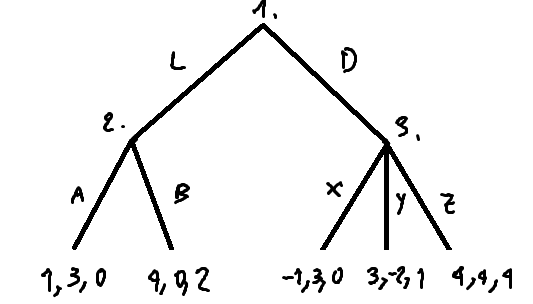
\includegraphics[scale=0.75]{drevo_1.png}
  \caption{Primer korenske igre}
\end{figure}

\begin{zgled}[Ultimatum game]
  Dva igralca si razdelita eno enoto. Prvi igralec da predlog oblike, da prvi dobi $x$ in drugi dobi $1 - x$.
  Drugi igralec lahko sprejme ali zavrne predlog. Če sprejme, si razdelita po predlogu prvega, sicer pa vsak dobi $0$.
  To igro spet predstavimo z drevesom, ki ima neskončno število vej iz korena. Drugi model
  pogajanja pa je naslednji: prvi igralec ponovno da predlog porazdelitve in če drugi zavrne, lahko da nasproten predlog.
  Prvi lahko nadalje sprejme ali pa da svoj novi predlog, in tako naprej v neskončnost.
  Pri tem se razdeljena količina zmanjšuje v vsaki rundi, pri čemer se lahko zmanjšuje aritmerično (v $(i+1)$-ti rundi si razdelita $1 - \varepsilon \cdot i$)
  ali pa geometrijsko (v $(1 + i)$-ti rundi si razdelita $1 \cdot (1 - \varepsilon)^i$). Slednja varianta lahko traja v neskončnost. 
  \begin{center}
    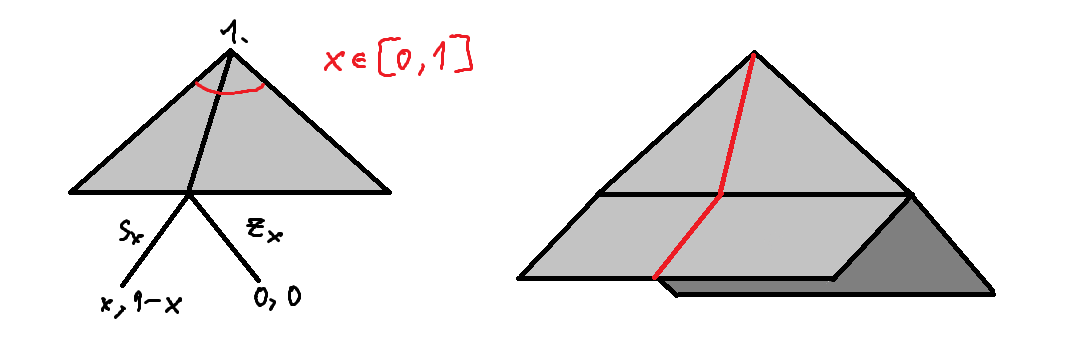
\includegraphics[scale=0.65]{drevo_2.png}
  \end{center}
\end{zgled}

\begin{definicija}
  Ekstenzivna igra je štirica $(N, T, P, (u_i)_{i \in N})$, pri čemer:
  \begin{itemize}
    \item $N$ množica igralcev,
    \item $T$ drevo s korenom, ki nima neskončne poti, njegova množica listov je $L(T)$,
    \item $P: V(T) \setminus L(T) \to N$ funkcija, ki pove, kdo je na vrsti v vozlišču $v$ in 
    \item $u_i: L(T) \to \R$ funkcija preferenc za igralca $i$.
  \end{itemize}
\end{definicija}

Povezave določijo akcije oziroma izbire igralcev. Označimo z $E_v$ množico povezav od vozlišča $v$ navzdol.
V vozlišču $v$ ima igralec $P(v)$ izbiro $E_v$. Strategija za igralca $i$ pove za vsako vozlišče, kjer je igralec $i$ na vrsti,
katere povezave bi izbral. Množica strategij za igralca $i$ je 
$$S_i = \prod_{v \in V(T) \setminus L(T),\ P(v) = i} E_v = \prod_{v \in P^{-1} (i)} E_v.$$
Množica profilov strategij je $S = \prod_{i \in N} S_i$.

\begin{zgled}
  Vzemimo za primer igro z naslednjim drevesom:
  \begin{center}
    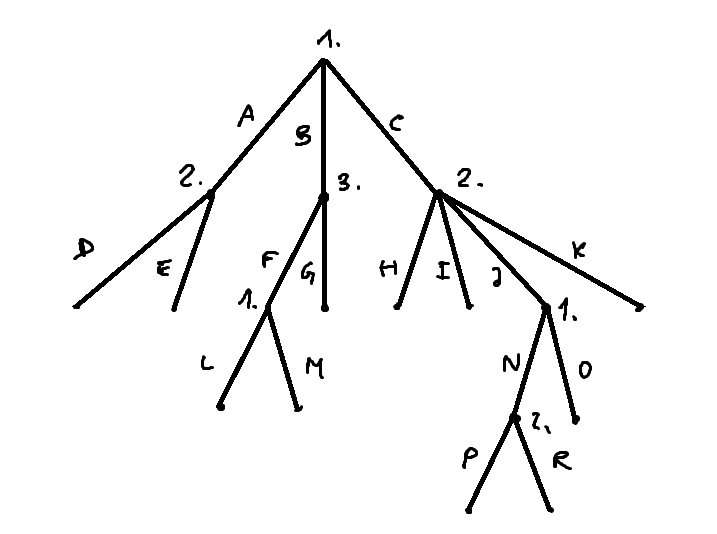
\includegraphics[scale=0.6]{drevo_3.png}
  \end{center}
  Potem je 
  $$S_1 = \{A, B, C\} \times \{L, M, N\} \times \{O, P\},$$
  torej ima igralec $3 \times 3 \times 2 = 18$ strategij. Podobno tudi za drugega igralca
  $$S_2 = \{D, E\} \times \{H, I, J, K\} \times \{Q, R\}$$ in pa za tretjega $S_3 = \{F, G\}$.
  Primer profila strategij iz $S_1 \times S_2 \times S_3$ je recimo $(\text{ALO}, \text{DKRG})$.
\end{zgled}

Definirajmo funkcijo izida (outcome) $O: S \to L(T)$, ki $(S_i)_{i \in N}$ preslika v list,
kjer se bo igra končala, če vsak igralec uporabi strategijo $S_i$.
To pa je tudi edini list, za katerega obstaja pot od korena v $$\bigcup_{i \in N,\ v \in V(T) \setminus L(T),\ P(v) = i} S_i (v).$$
Profil $s^* = (S_i^*)_{i \in N} \in S$ je Nashevo ravnovesje natanko tedaj, ko velja 
$$\forall i \in N:\ \forall s_i' \in S_i:\ u_i (O((S_j^*)_{j \in N})) \geq u_i (O((S_j^*)_{j \in N}\ |\ S_i'))$$ 
oziroma $u_i (O(s^*)) \geq u_i (O(s^*\ |\ s_i))$. Kot v večih primerih do sedaj imamo 
funkcijo 
$$\Phi_{\text{eks $\to$ pref}}: \{\text{ekstenzivne igre}\} \to \{\text{strateške igre s funkcijami preferenc}\}$$
s predpisom $$(N, T, P, (u_i)_{i \in N}) \mapsto (N, (S_i)_{i \in N}, (u_i \circ O)_{i \in N}).$$
Nashevo ravnovesje v ekstenzivni igri $\Gamma$ je Nashevo ravnovesje v strateški igri s funkcijami preferenc 
$\Phi_{\text{eks $\to$ pref}}(\Gamma)$.

\begin{zgled}[Threatening game]
  Igro z drevesom 
  \begin{center}
    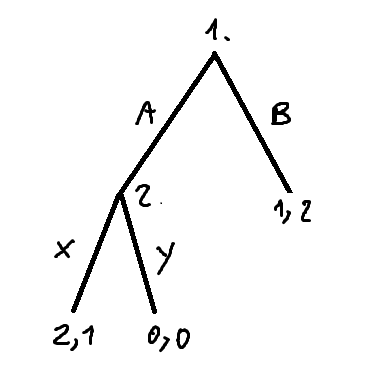
\includegraphics[scale=0.7]{drevo_4.png}
  \end{center}
  preoblikujemo v tabelo 
  $$  
  {\begin{tabular}{c|c|c|c|}
    & \textrm{X} & \textrm{Y}\\
    \hline
    \textrm{A} & 2, 1 & 0, 0\\
    \hline
    \textrm{B} & 1, 2 & 1, 2\\
    \hline
  \end{tabular}}
  $$
  Nashevi ravnovesji sta pri $(A, X)$ in $(B, Y)$. Trdimo, da bo drugi igralec igral slabše, zato da bi grozil prvemu,
  da igra $B$. Včasih pa s takim modeliranjem iger nismo zadovoljni, zato vpeljemo nov koncept ravnovesja.
\end{zgled}

Vpeljemo koncept ugnezdenega Nashevega ravnovesja\footnote{subgame perfect equilibrium}.
Ideja je naslednja: uporabimo Nashevo ravnovesje za vsako podigro oziroma od vsakega vozlišča navzdol.
Za poljubno vozlišče $v \in V(T) \setminus L(T)$ definiramo funkcijo $O_v: S \to L(T)$,
ki $(S_i)_{i \in N}$ preslika v list drevesa, kjer se konča igra, če začnemo v vozlišču $v$ in igralci 
uporabijo $S_i, \forall i \in N$. Profil strategij $s^* = (S_i^*)_{i \in N} \in S$ 
je vgnezdeno Nashevo ravnovesje, če velja 
$$\forall v \in V(T) \setminus L(T):\ \forall i \in N:\ \forall s{_i}' \in S_i:\ u_i (O_v(s^*)) \geq u_i (O_v(s^*\ |\ s{_i}' )).$$
V zgledu je torej $(A, X)$ vgnezdeno Nashevo ravnovesje, $(B, Y)$ pa ne. V splošnem poiščemo vzgnezdeno Nashevo 
ravnovesje tako, da naredimo povratno indukcijo (dinamično programiranje) in od spodaj navzdol pogledamo vse podigre.

\subsection{Zgledi}

\begin{zgled}
  Vzemimo igro z naslednjim drevesom:
  \begin{center}
    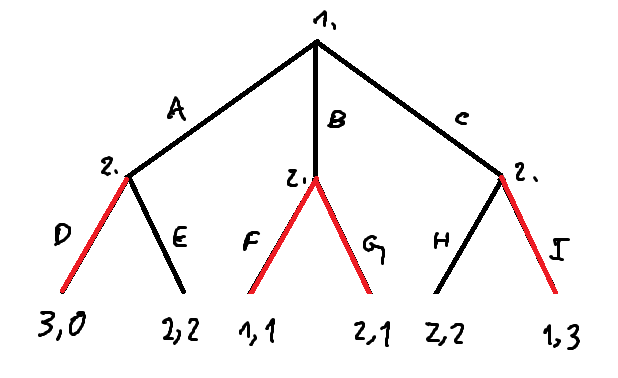
\includegraphics[scale=0.7]{drevo_5.png}
  \end{center}
  Množica strategij za prvega igralca je $S_1 = \{A, B, C\}$, za drugega igralca pa 
  $$S_2 = \{D, E\} \times \{F, G\} \times \{I, H\}.$$
  V igri $\Gamma(v_1)$ drugi igralec igra $E$, v igri $\Gamma(v_2)$ igra bodisi $F$ bodisi $G$,
  v igri $\Gamma(v_3)$ pa igra $H$. Torej imamo vgnezdena Nasheva ravnovesja $(\text{A}, \text{EFH})$, $(\text{A}, \text{EGH})$ in $(\text{B}, \text{EGH})$.
\end{zgled}

\begin{zgled}
  Vrnimo se na začetno verzijo igre ultimatum game.
  V igri $\Gamma(v_x)$ bo drugi igralec igral
  $$\begin{cases}
    S_x;& x \neq 1\\
    \text{$S_x$ ali $Z_x$};& x = 1
  \end{cases}.$$
  Na voljo ima torej dve strategiji: $s_2$, kjer vedno sprejme ponudbo, in $s_2'$, kjer vedno sprejme ponudbo, razen ko je $x = 1$.
  Za prvo strategijo obstaja vgnezdeno Nashevo ravnovesje, ko prvi igralec izbere $x = 1$, če pa drugi igralec izbere drugo strategijo, pa vgezdenega Nashevega ravnovesja ni.
\end{zgled}

\begin{zgled}
  Oglejmo si ekstenzivno igro z drevesom 
  \begin{center}
    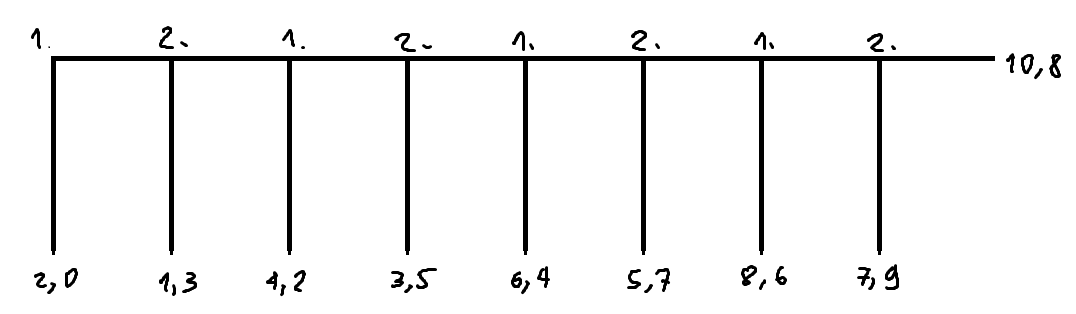
\includegraphics[scale=0.6]{drevo_6.png}
  \end{center}
  Vgnezdeno Nashevo ravnovesje te igre je kar, če prvi igralec igro takoj konča.
  Ta igra je bila tudi predmet eksperimenta, v katerem so bili igralci dejanski ljudje.
  Izkazalo se je, da se je s številom ponovitev iger dolžina igre zmanjševala.
\end{zgled}

\begin{zgled}[Stackelbergov model duopola]
  Stackelbergov model je modifikacija Cournotovega modela,
  kjer prva firma izbere $q_1$ in nato druga firma izbere $q_2$.
  Pri tem druga firma že ve, kaj je izbrala prva firma.
  Funkcija cene je ponovno $P(q_1 + q_2) = (P_{\max} -q_1 -q_2)_+$,
  dobiček pa je $u_i (q_1, q_2) = q_i(P(q_1 + q_2) - c)$.
  Ponovno tudi predpostavimo, da je $P_{\max} > c >0$.
  Sedaj to modeliramo kot ekstenzivno igro in poiščemo njeno vgnezdeno Nashevo ravnovesje.
  Iščemo torej 
  $$\max_{q_2 \in [0, \infty)} u_2 (q_1, q_2) = \max_{q_2 \in [0, \infty)} q_2 ((P_{\max} - q_1 - q_2)_+ - c).$$
  Pri analizi Cournotovega modela smo izračunali najboljši odgovor za drugega igralca:
  $$B_2 (q_1) = \begin{cases}
    \frac{P_{\max} - c - q_1}{2};& P_{\max} - c- q_1 > 0\\
    0;& \textrm{sicer}
  \end{cases},$$
  ki je zvezna funkcija. Če torej obstaja vgnezdeno Nashevo ravnovesje, bo druga firma uporabila strategijo $S_2$, 
  na katero gledamo kot preslikavo 
  $$q_1 \mapsto \left(\frac{P_{\max} - c - q_1}{2}\right)_+.$$
  Prva firma pa zato izbere 
  $$\max_{q_1 \in [0, \infty)} u_1 (q_1, s_2 (q_1)) = \max_{q_2 \in [0, \infty)} q_1 \left(\left(P_{\max} - q_1 - \left(\frac{P_{\max} - c- q_1}{2}\right)_+\right)_+ - c\right).$$
  Če velja $P_{\max} - c - q_1 \geq 0$, potem je to enako 
  $$\max_{q_1 \in [0, \infty)} \frac{1}{2} q_1 (P_{\max} - q_1).$$
  Ta funkcija pa ima maksimum pri $q_1 = \frac{P_{\max} - c}{2}$, za ta $q_1$ velja $P_{\max} - c - q_1 \geq 0$, torej 
  res ustreza pogojem. Če sedaj dobljeno vstavimo v funkcijo preferenc, dobimo 
  $$u_1\left(\frac{P_{\max} - c}{2}, \left(\frac{P_{\max} - c - \frac{P_{\max} - c}{2}}{2}\right)\right) = \frac{1}{8} (P_{\max} - c)^2 > 0.$$ 
  Obravnvati moramo še primer, ko je $P_{\max} - c - q_1 < 0$.
  Tedaj je $q_2 = 0$ in prva firma bo dobila 
  $$q_1 ((P_{\max} - q_1)_+ - c) \leq 0.$$
  Torej je najboljša izbira za prvega igralca enaka $q_1 = \frac{P_{\max} - c}{2}$
  in dobimo vgnezdeno Nashevo ravnovesje 
  $$\left(q_1 = \frac{P_{\max} - c}{2}, q_2 = \left(\frac{P_{\max} - c - q_1}{2}\right)_+\right).$$
  Pri vgnezdenem Nashevem ravnovesju bo $q_1 = \frac{P_{\max} - c}{2}$ in $q_2 = \frac{P_{\max} - c}{4}$, od koder dobimo 
  $$u_1 = \frac{1}{8} (P_{\max} - c)^2,\quad u_2 = \frac{1}{16} (P_{\max})^2.$$
  To se tudi ujema z našo intuicijo, da bo prva firma (market leader)
  zaslužila več kot druga (market follower).
\end{zgled}

\begin{zgled}[Entry deterrance]
  Opazujemo primer Stackelbergovega duopola, kjer bo prva firma izbrala $q_1$ tako, da druga firma nikoli ne bo začela proizvajati.
  Naj bo dana funkcija cene 
  $$P(q_1 + q_2) = 17 - q_1 - q_2$$
  (dobimo isto vgnezdeno Nashevo ravnovesje, kot če bi vzeli $(17 - q_1 - q_2)_+$).
  in stroški za $i$-to firmo:
  $$\begin{cases}
    o;& q_i = 0\\
    q + q_i;& q_i > 0
  \end{cases},$$
  kjer $q > 0$ predstavlja začetne stroške.
  Dobiček fire $i$ je 
  \begin{align*}
    u_i (q_1, q_2) &= \begin{cases}
      q_i (17 - q_1 - q_2 - 1) - 9; & q_i > 0\\
      0;& q_i = 0
    \end{cases}\\
    &= \begin{cases}
      q_i (16 - q_1 - q_2) - 9;& q_i > 0\\
      0;& q_i = 0.
    \end{cases}
  \end{align*}
  Ponovno začnemo z iskanjem Nashevega ravnovesja vgnezdene igre:
  $$\max_{q_2 \in [0, \infty)} u_2(q_1, q_2) = \max_{q_2 \in [0, \infty)} \begin{cases}
    q_i (16 - q_1 - q_2) - 9;& q_i > 0\\
    0;& q_i = 0.
  \end{cases}$$
  Funkcija $q_2 (16 - q_1 - q_2) - 9$ ima maksimum pri $q_2 = \frac{16 - q_1}{2}$,
  kjer je njena vrednost enaka $\left(\frac{16 - q_1}{2}\right)^2 - 9$. Imamo 
  $$\left(\frac{16 - q_1}{2}\right)^2 - 9 \geq 0 \Leftrightarrow q_i \in \stcomp{(10, 22)}.$$
  Tako dobimo najboljši odgovor za drugega igralca
  $$B_2 (q_1) = \begin{cases}
    \frac{16 - q_1}{2};& q_1 < 10\\
    \{0, 3\};& q_1 = 10\\
    0;& q_1 > 10
  \end{cases}.$$
  Druga firma ima dve strategiji, ki se lahko pojavijo v vgnezdenem Nashevem ravnovesju:
  $$S_2 = \begin{cases}
    q_2 = \frac{16 - q_1}{2};& q_1 < 10\\
    q_2 = 0;& q_1 \geq 10
  \end{cases},\quad S_2' = \begin{cases}
    q_2 = \frac{16 - q_1}{2};& q_1 \leq 10\\
    q_2 = 0;& q_1 > 10
  \end{cases}.$$
  Najprej predpostavimo, da prva igra uporabi strategijo $S_2$.
  Ali potem obstaja vgnezdeno Nashevo ravnovesje? Prva firma igra:
  $$\max_{q_1 \in [0, \infty)} u_1 (q_1, S_2(q_1)) =\max_{q_1 \in [0, \infty)} \begin{cases}
    q_1 \left(\frac{16 - q_1}{2}\right) - 9;& q_1 < 10\\
    q_1 (16 - q_1) - 9;& q_1 \geq 10.
  \end{cases}$$
  Maksimum je dosežen pri $q_1 = 10$, kjer je vrednost enaka $51$.
  Torej smo dobili vgnezdeno Nashevo ravnovesje 
  $(q_1 = 10, S_2)$. Pri tem vgnezdenem Nashevem ravnovesju igra $q_1 = 10$ in $q_2 = 0$.
  Sedaj si oglejmo še primer, ko druga firma uporabi $S_2'$. Potem iščemo 
  $$\max_{q_1 \in[0, \infty)} u_1 (q_1, S_2'(q_1)) = \max_{q_1 \in [0, \infty)} \begin{cases}
    q_1 \left(\frac{16 - q_1}{2}\right) - 9;& q_1 \leq 10\\
    q_1 (16 - q_1);& q_1 > 10
  \end{cases}.$$
  Ta maksimum pa ne obstaja, saj vrednost $51$ ni nikoli dosežena.
\end{zgled}

\begin{zgled}[Stackelberg pricing problems]
  Denimo, da imamo graf, ki vsebuje vozlišči $s$ in $t$ in našo povezavo $e$.
  Izbrati želimo ceno naše povezave $e$, tako da bo najcenejša pot skozi ta graf (z uteženimi povezavami)
  potekala skozi $e$. To lahko tudi posplošimo, tako da imamo več različnih parov $s_i, t_i$
  in promet $p_i$. Potem v odvisnosti od cene naše povezave iščemo maksimum vsote produktov $$p_i \cdot (\textrm{cena povezave})$$ po indeksih
  $i$, za katere najcenejša $s_i-t_i$ pot v grafu poteka skozi povezavo $e$.  
\end{zgled}

\begin{zgled}
  Oglejmo si kombinacijo ekstenzivnih in strateških iger s funkcijami preferenc.
  \begin{center}
    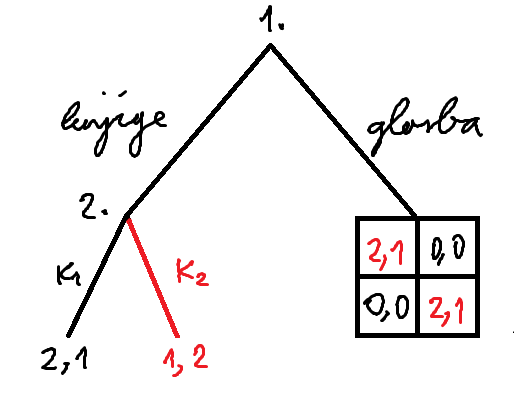
\includegraphics[scale=0.8]{drevo_7.png}
  \end{center}
  Tako dobimo tri vgnezdena Nasheva ravnovesja: 
  $$((\mathrm{glasba}, B), (B, K_2)),\quad ((\mathrm{glasba}, S), (S, K_2)), \quad ((\mathrm{knjige}, S), (S, K_2)).$$
  Če pa imamo funkcije koristnosti, potem ima igra Bach in Stravinsky še eno mešano Nashevo ravnovesje;
  poiščemo ga s principom indiferentnosti.
  $$p + 0 = 0 + 2(1 - p) \Rightarrow p = \frac{2}{3}.$$
  Tako dobimo mešano Nashevo ravnovesje:
  $$\left(\begin{pmatrix}
    B & S\\ 2/3 & 1/3
  \end{pmatrix}, \begin{pmatrix}
    B & S\\ 1/3 & 2/3
  \end{pmatrix}\right),$$
  pri katerem dobita oba igralca $\frac{2}{3}$.
  Sedaj pa imamo vgnezdeno Nashevo ravnovesje 
  $$\left(\left(\mathrm{knjiga}, \begin{pmatrix}
    B & S\\ 2/3 & 1/3
  \end{pmatrix}\right), \left(\begin{pmatrix}
    B & S\\ 1/3 & 2/3
  \end{pmatrix}, K_2\right)\right).$$
\end{zgled}

\begin{zgled}[Rekurzivne igre]
  Oglejmo si igro, podano z 
  $$
    \Gamma = {\begin{tabular}{|c|c|}
        \hline
        $\Gamma_1$ & 4\\
        \hline
        5 & $\Gamma_2$\\
        \hline
    \end{tabular}}, \quad         
    \Gamma_1 = {\begin{tabular}{|c|c|}
      \hline
      0 & 3\\
      \hline
      2 & -1\\
      \hline
  \end{tabular}},\quad 
  \Gamma_2 = {\begin{tabular}{|c|c|}
    \hline
    0 & 1\\
    \hline
    4 & 3\\
    \hline
\end{tabular}}.
$$
Tukaj seveda oba igralca mešata.
\end{zgled}

\begin{zgled}
  Prejšnji zgled lahko posplošimo na neskončno rekurzijo.
  Oglejmo si recimo rekurzivno igro 
  $$\Gamma = {\begin{tabular}{|c|c|}
    \hline
    $\Gamma$ & 1\\
    \hline
    1 & 2\\
    \hline
\end{tabular}}.$$
Če igralca izbereta strategiji 
$$\left(\begin{bmatrix}
  p \\ 1 - p
\end{bmatrix}, \begin{bmatrix}
  q\\ 1 - q
\end{bmatrix}\right),$$
potem bo izid ustrezal enačbi 
$$\mathrm{izid} (p, q) = pq\, \mathrm{izid} (p, q) + p(1 - q) + q (1 - p) + 2(1 - p)(1 - q).$$
S tem bo izid določen za vse strategije obeh igralcev, razen za
$p = q = 1$, saj takrat igra poteka v neskončnost. Zato moramo zraven igre še posebej določiti izid v 
primeru, ko igra poteka v nedogled. Vgnezdeno Nashevo ravnovesje je seveda potem odvisno tudi od te določene vrednosti.
Seveda lahko naše pojme posplošujemo še naprej. Lahbo bi recimo imeli matriki 
$$\Gamma_1 = {\begin{tabular}{|c|c|}
  \hline
  $\Gamma_2$ & 1\\
  \hline
  1 & 2\\
  \hline
\end{tabular}},\quad \Gamma_2 = 
{\begin{tabular}{|c|c|}
  \hline
  $\Gamma_1$ & 1\\
  \hline
  1 & 2\\
  \hline
\end{tabular}}.$$
Možnosti za posplošitev so res neomejene.
\end{zgled}

\section{Ekstenzivne igre z nepopolno informacijo}

V tem razdelku modeliramo ekstenzivne igre, pri katerih
določeni igralci ne vedo, na katerem vozlišču (v informacijski množici) so.
Posameznega igralca si lahko recimo predstavljamo kot 
skupino ljudi z istim interesom, ki pa morda med seboj ne komunicirajo.
\begin{figure}[hbt!]
  \centering
  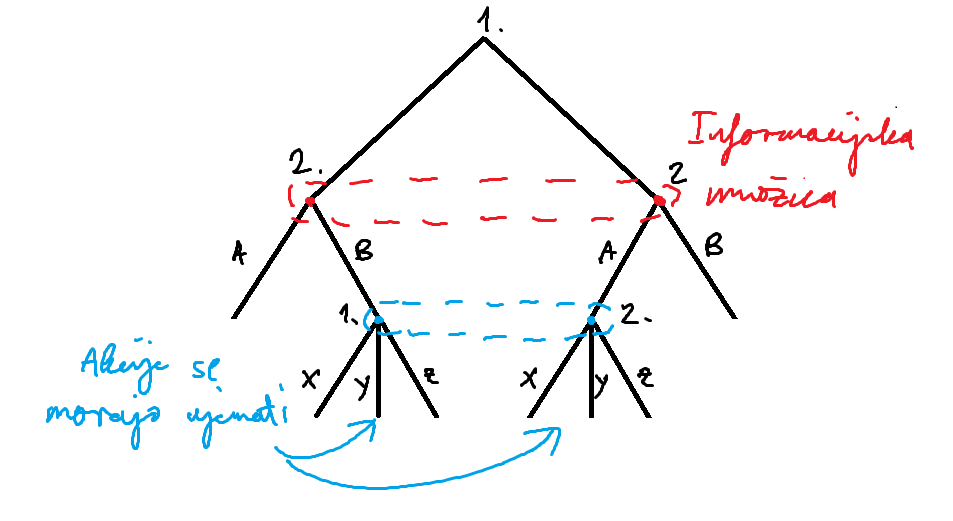
\includegraphics[scale=0.7]{drevo_8.png}
  \caption{Primer ekstenzivne igre z nepopolno informacijo}
\end{figure}
Povsem formalna definicija bi bila naslednja.

\begin{definicija}
  Ekstenzivna igra z nepopolno informacijo je peterica $(N, T, P, \mathcal{H}, (u_i)_{i \in N})$, kjer je:
  \begin{itemize}
    \item $(N, T, P, (u_i)_{i \in N})$ ekstenzivna igra s popolno informacijo.
    \item $\mathcal{H} = \{H_1, H_2, \dots, H_n\}$ množica informacijskih particij igralcev,
    kjer je za $i$-tega igralca $H_i = \{H_{i, 1}, H_{i, 2}, \dots, H_{i, k_i}\}$ particija množice $\{v \in V(T)\setminus L(T)\ |\ P(v) = i\}$,
    tako da je za vsak $H_{i, j}$ množica akcij $A(h) = A(h')$ za poljubni $h, h' \in H_{i, j}$.
  \end{itemize}
\end{definicija}

Kadar si vsak igralec zapomni svoje prejšnje poteze, pravimo, da igramo "`game with perfect recall"',
v nasprotnem primeru pa "`game with imperfect recall."'

\begin{figure}[hbt!]
  \centering
  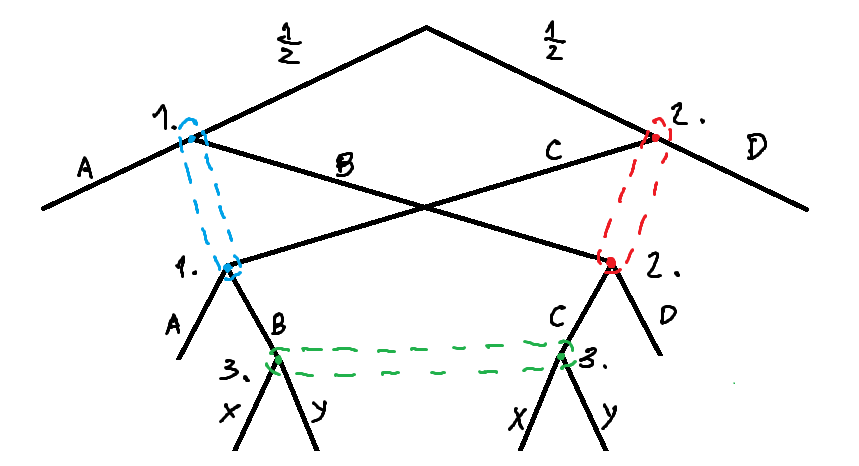
\includegraphics[scale=0.7]{drevo_9.png}
  \caption{Primer igre, kjer ima vsak igralec "`perfect recall"'}
\end{figure}

Za več o tem si poglej knjigo Game Theory Basics avtorja Bernharda von Stengela.

\section{Nashev model pogajanja}

V kooperativnih igrah je več igralcev, ki lahko podpišejo sporazum 
(angl. \emph{binding agreement}).
Ko igralci sklenejo dogovor in podpišejo sporazum, potem je igre konec in vsakdo dobi,
kar izhaja iz sporazuma. Ta pa lahko tudi uporabi verjetnost.
Igralci lahko na primer sklenejo, katere mešane sporazume bo uporabil vsak igralec v strateški igri.
Če igralca skleneta sporazum, potem igra ni več pod kontrolo igralcev in nek sodnik 
avtomatično implementira sporazum. V tem poglavju bomo raziskali 
strateške igre za dva igralca, kjer lahko ta sodelujeta.
Take igre bomo študirali z vidika Nashevega modela pogajanja (angl. \emph{Nash bargaining solution}).

\subsection{Osnovni koncepti}

\begin{zgled}\label{zgl:1}
  Oglejmo si bimatrično igro 
$$[A, B] = \begin{bmatrix}
  1,5 & 4,4\\
  2,1 & 6,0
\end{bmatrix}.$$
Edino Nashevo ravnovesje te igre je pri $(\delta(2), \delta(1))$,
kjer igralca dobita izplačilo $(2, 1)$. Po drugi strani pa bi bilo za igralca bolje,
če bi igrala $(\delta(1), \delta(2))$, saj bi tedaj dobila boljši izkupiček.
\end{zgled}

Pri tem modelu seveda predpostavimo, da nobeden od igralcev svoje izbire ne more naknadno spremeniti.
Ker igralca ne dobita enake koristi od tega sporazuma, v model vključimo morebitna stranska plačila 
(\emph{side payments}). Da so taka stranska plačila sploh smiselna,
pa morata oba igralca uporabiti iste enote.
Če imata igralca funkciji koristnosti izražena v istih enotah,
pravimo, da je koristnost prenosljiva in lahko sporazum določi stransko plačilo,
v nasprotnem primeru pa je koristnost neprenosljiva.

\begin{zgled}
  Za primer si oglejmo matrično igro
  $$[A, B] = \begin{bmatrix}
    1,9 & 2,2\\
    2,2 & 9,1
  \end{bmatrix}.$$
  Tukaj bosta igralca težko sklenila dogovor, katero strategijo naj uporabita,
  zato bi lahko podpisala sporazum, ki določa, da je izid igre bodisi $(\delta(1), \delta(1))$
  bodisi $(\delta(2), \delta(2))$ z enako verjetnostjo.
\end{zgled}

Naj bo sedaj $[A, B]$ poljubna bimatrična igra velikosti $m \times n$, kjer 
uporabimo notacijo $(a_{i, j}, b_{i, j}) = [A, B]_{i, j}$ za vsak $(i, j) \in [m] \times [n]$.
Če je koristnost neprenosljiva, bosta igralca podpisala naslednji sporazum, kjer bo izid izbran naključno 
s funkcijo verjetnosti $\pi \in \Pi ([m] \times [n])$.
To pomani, da bo izid pri $(i, j)$ izbran z verjetnostjo $\pi(i, j)$,
pri čemer velja $\sum_{i, j} \pi (i, j) = 1.$
Pri takem sporazumu igralec $1$ pričakuje koristnost 
$$a = a(A, \pi) = \sum_{i, j} \pi(i, j) \cdot a_{i, j}$$
in podobno drugi tudi igralec:
$$b = b(B, \pi) = \sum_{i, j} \pi(i, j) \cdot b_{i, j}.$$
Tak sporazum bomo kar identificirali s funkcijo verjetnosti $\pi$.
Če pa je koristnost prenosljiva, pa je sporazum opisan s parom $(T, \pi) \in \R \times \Pi([m] \times [n])$,
kjer je $\pi$ funkcija verjetnosti kot prej, $T$ pa izkupiček, ki igralec $1$ plača igralcu $2$.
Če podpišeta takšen sporazum, potem prvi igralec pričakuje 
$$a = a(A, T, \pi) = -T + \sum_{i, j} \pi(i, j) \cdot a_{i, j}$$
enot koristnosti, igralec $2$ pa 
$$a = b(A, T, \pi) = T + \sum_{i, j} \pi(i, j) \cdot b_{i, j}$$
enot koristnosi. V obeh primerih pa rečemo, da je $(a, b)$ rezultat sporazuma.
V primeru neprenosljive koristnosti definiramo množico dopustnih rezultatov 
$$D_{\mathrm{NPK}} (A, B) = \{(a(\pi), b(\pi)) \in \R^2\ |\ \pi \in \Pi([m] \times [n])\},$$
ki jo lahko ekvivalentno zapišemo kot 
$$\{(a, b)\in \R^2\ |\ \exists \pi \in \Pi([m] \times [n]),\ (a, b) \in \sum_{i, j} \pi(i, j) \cdot (a_{i, j}, b_{i, j})\},$$
kar pa je natanko konveksna ovojnica množice točk 
$$\{(a_{i, j}, b_{i, j})\ |\ (i, j) \in [m] \times [n]\}.$$
Za prenosljive koristnosti pa definiramo množico dopustnih rezultatov kot 
\begin{align*}
  D_{\mathrm{PK}} (A, B) &= \{(a - s, b + s) \in \R^2\ |\ (a, b) \in D_{\mathrm{NPK}}, s \in \R\}\\
  &= \{(a, b) \in \R^2\ |\ \min_{i, j} (a_{i, j} + b_{i, j}) \leq a + b \leq \max_{i, j} (a_{i, j} + b_{i, j})\}.
\end{align*}

\begin{figure}
  \centering
  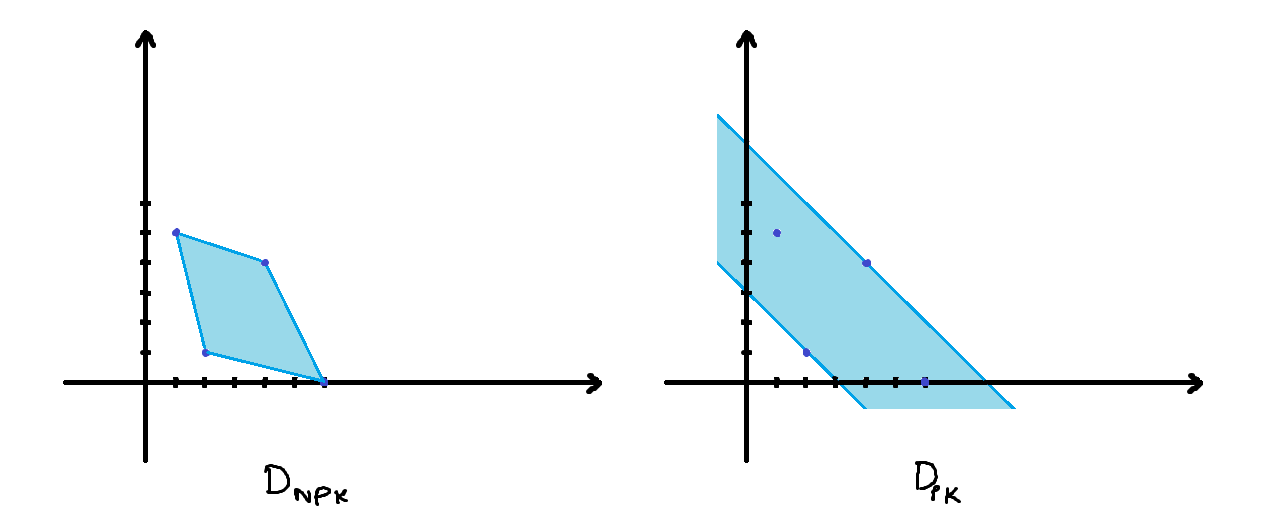
\includegraphics[scale=0.7]{images/slika4.png}
  \caption{Množici dopustnih rezultatov za igro iz zgleda \ref{zgl:1}}
\end{figure}

\subsection{Nashev produkt}

Naj bo $K$ kompaktna konveksna množica v ravnini in $(x_0, y_0)$ neka poljubna točka v ravnini 
(pri tem ne zahtevamo, da je $(x_0, y_0) \in K$, čeprav bo v veliko primerih to res držalo).
Denimo, da ima $K$ neko točko $(x, y)$, za katero velja $x \geq x_0$ in $y \geq y_0$.
Oglejmo si sedaj Nashev produkt $(x - x_0) (y - y_0)$ za točke $(x, y) \in K$.
Sedaj lahko opazimo, da je krivulja $(x - x_0) (y - y_0) = c$
hiperbola za poljubno konstanto $c \in \R$. Zanimal nas bo optimizacijski problem 
$$\Phi(K, x_0, y_0) = \sup (x - x_0) (y - y_0)\qquad \text{pri pogojih}\ (x, y) \in K,\ x \geq x_0, y\geq y_0.$$
Najprej dokažimo, da lahko supremum zamenjamo z maksimumom in je ta dosežen le v eni točki,
ki jo označimo $N(K, x_0, y_0)$.

\begin{trditev}
  Naj bo $K$ kompaktna in konveksna množica v $\R^2$ in $(x_0, y_0) \in \R^2$ poljubna točka.
  Denimo, da obstaja točka $(x, y) \in K$, za katero velja $x > x_0$ in $y > y_0$.
  Potem obstaja enolična točka $(x^*, y^*) \in K$, za katero velja
  $$(x^* - x_0) (y^* - y_0) = \Phi(K, x_0, y_0).$$
\end{trditev}

\begin{dokaz}
  Naj bo $$K_{\geq} = \{(x, y) \in K\ |\ x \geq x_0, y \geq y_0\}$$
  in označimo $\Phi = \Phi(K, x_0, y_0)$ znotraj tega dokaza.
  Ker je vsaj ena točka $(x, y) \in K$, za katero velja $x > x_0$ in $y > y_0$, mora biti $\Phi > 0$.
  Množica $K_{\geq}$ je kompaktna in $(x - x_0) (y - y_0)$ je zvezna funkcija, zato res obstaja vsaj ena točka 
  $(x^*, y^*) \in K_{\leq}$, za katero velja $\Phi = (x^* - x_0)(y^* - y_0)$.
  Preveriti moramo še, da je taka točka res enolično določena.
  Denimo, da obstajata različni točki $(x_1, y_1),(x_2, y_2) \in K_{\leq}$,
  kjer je maksimum dosežen, in naj bo $d$ daljica med tema dvema točkama.
  Ker sta $(x_1, y_1)$ in $(x_2, y_2)$ na delu hiperbole $(x - x_0)(y - y_0) = \Phi > 0$,
  ima daljica $d$ negativen naklon. Ker je $K_{\geq}$ konveksna, je daljica $d$ 
  seveda vsebovana v tej množici. Sedaj pa uporabimo dejstvo, da je funkcija 
  $(x - x_0) (y - y_0)$ konkavna na daljici $d$ in dobimo protislovje s predpostavko, da je $\Phi$
  maksimum na množici $K_{\geq}$.
\end{dokaz}

\begin{figure}
  \centering
  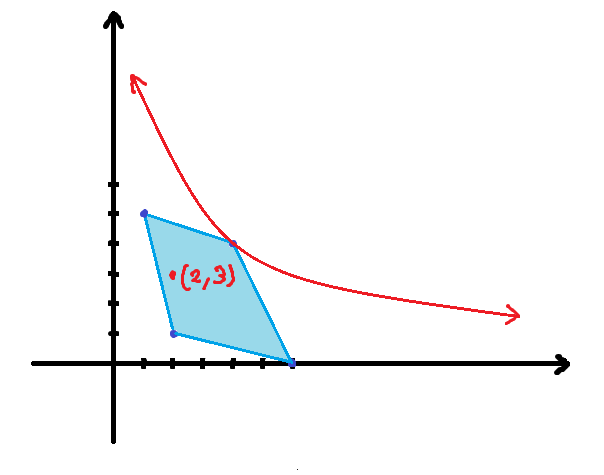
\includegraphics{images/slika5.png}
  \caption{Nashev produkt iz zgleda \ref{zgl:1}, kjer je $(x_0, y_0) = (2, 3)$}
  \label{fig:1}
\end{figure}

Krivulja $$(x - x_0)(y - y_0) = \Phi(K, x_0, y_0)$$
se dotika množice $K$ (glej sliko \ref{fig:1}) bodisi v točki v oglišču bodisi v enem izmed robov.
Za edino rešitev zgornjega optimizacijskega problema uporabimo oznako $N(K, x_0, y_0)$.
Na sliki \ref{fig:1} je $N(K, 2, 3) = (4, 4)$. Z naslednjo trditvijo dobimo orodje za izračun te točke,
ko je $K$ konveksen večkotnik. Tehnika dokaza je uporabna za konveksne množice, ki imajo odvedljiv rob.

\begin{trditev}\label{trd:1}
  Naj bo $T$ trikotnik z oglišči $(0, 0)$, $(X, 0)$ in $(0, Y)$,
  kjer velja $X, Y > 0$. Potem je $N(T, 0, 0) = \left(\frac{X}{2}, \frac{Y}{2}\right)$.
\end{trditev}

\begin{dokaz}
  Naj bo $x^*, y^*$ optimalna rešitev naloge za $N(T, 0, 0)$
  in naj bo $\Phi = x^* y^*$. To pomeni, da je krivulja $xy = \Phi$ tangentna premici 
  $y = Y - \frac{Y}{X}x$, ki vsebuje hipotenuzo trikotnika $T$ in 
  ima naklon $-\frac{Y}{X}$. Tangenta krivulje $y = \frac{\Phi}{x}$
  pri točki $(x^*, y^*)$ je $-\frac{\Phi}{(x^*)^2}$.
  Tako dobimo sistem enačb 
  $$-\frac{Y}{X} = - \frac{\Phi}{(x^*)^2},\quad y^* = Y - \frac{Y}{X} x,\quad \Phi = x^* y^*,$$
  katerega rešitev je $(x^*, y^*, \Phi) = \left(\frac{X}{2}, \frac{Y}{2}, \frac{XY}{4}\right)$.
\end{dokaz}

\begin{trditev}\label{trd:2}
  Naj bosta $f_1 (x) = \alpha_1 x + \beta_1$ in $f_2 (x) = \alpha_2 x + \beta_2$,
  kjer sta $\alpha_1, \alpha_2 > 0$.
  Za poljubno konveksno množico $K$
  definiramo $K_f = \{(f_1 (x), f_2 (x))\in \R^2\ |\ (x, y) \in K\}$.
  Potem je za vsako točko $(x_0, y_0)$
  $$N(K_f, f_1(x_0), f_2 (x_0)) = (f_1 (x^*), f_2 (y^*)),$$
  pri čemer je $(x^*, y^*) = N(K, x_0, y_0)$.
\end{trditev}

\begin{dokaz}
  Denimo, da je točka $N (K_f, f_1(x_0), f_2 (x_0))$ enolična rešitev našega optimizacijskega problema 
  $\max (x' - f_1 (x_0)) (y' - f_2(y_0))$ pri pogojih 
  $$(x', y') \in \{(x', y') \in K_f\ |\ x' \geq f_1 (x_0), y' \geq f_2 (y_0)\}.$$
  Če sedaj vpeljemo spremembi koordinat $(x', y') = (f_1 (x), f_2 (y))$, dobimo optimizacijski problem
  $\max (f_1(x) - f_1 (x_0)) (f_2(y) - f_2(y_0))$ pri pogojih 
  $$(x, y) \in \{(x, y) \in K_f\ |\ f_1(x) \geq f_1 (x_0), f_2(y) \geq f_2 (y_0)\}.$$
  Če pa sedaj upoštevamo še definiciji funkcij $f_1, f_2$, dobimo problem 
  $\max \alpha_1 (x -x_0) \alpha_2(y - y_0)$ pri pogojih 
  $$(x, y) \in \{(x, y) \in K_f\ |\ \alpha_1 x \geq \alpha_1 x_0, \alpha_2 y \geq \alpha_2 y_0\}.$$
  V zadnjem problemu je takoj očitno, da je maksimum dosežen pri $(x^*, y^*) = N(K, x_0, y_0)$
  in nato iz spremembe koordinat sledi, da je optimalna točka problema dosežena v točki 
  $(f_1(x^*), f_2(y^*))$.
\end{dokaz}

\begin{zgled}
  Denimo, da imamo množico $K$, podano na sliki.
  \begin{center}
    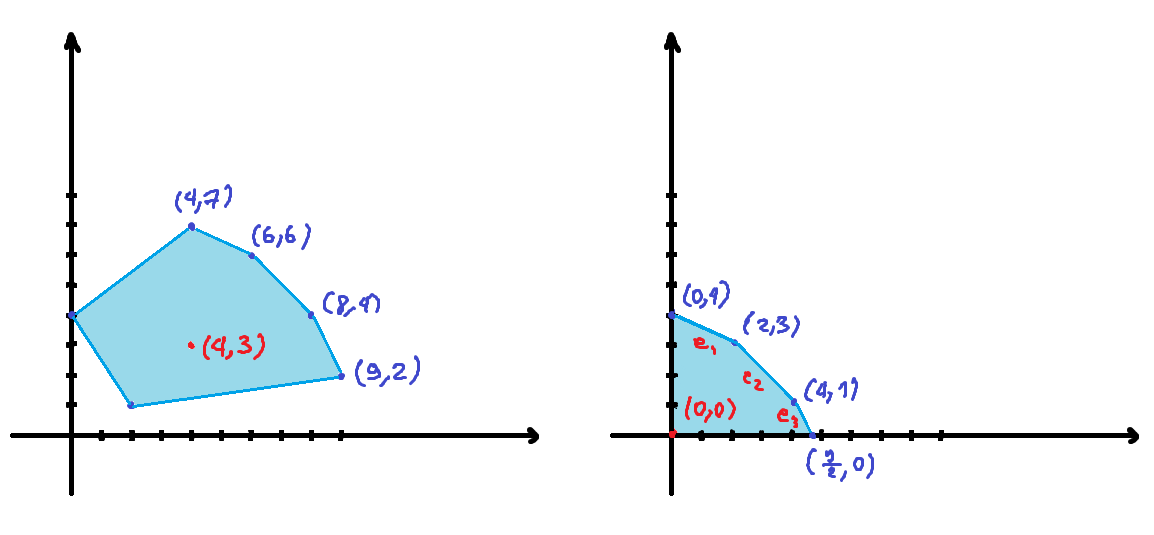
\includegraphics[scale=0.6]{images/slika6.png}
  \end{center}
  Najprej lahko uporabimo prejšnjo trditev in naredimo translacijo,
  ki pošlje točko $(4, 3)$ v $(0, 0)$ in nato iščemo $N(K', 0, 0)$,
  kjer smo označili množico $$K' = \{(x, y)\ |\ (x + 4, y + 3) \in K\}.$$
  Nato označimo z $e_1, e_2, e_3$ robove, kjer lahko leži $N(K', 0, 0)$.
  \begin{center}
    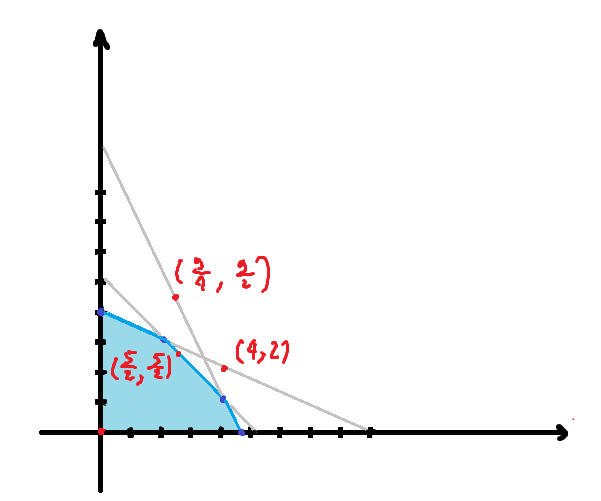
\includegraphics[scale=0.8]{images/slika7.png}
  \end{center}
  Za $i = 1, 2, 3$ naj bo $T_i$ trikotnik, ki ga določa rob $e_i$ in obe koordinatni osi.
  Trikotnik $T_i$ ima tako oglišča $(0, 0)$, $(8, 0)$ in $(0, 4)$.
  Če je $N(K', 0, 0)$ na robu $e_i$, potem je tudi na robu trikotnika $T_i$.
  Tako lahko uporabimo trditev \ref{trd:1}, da dobimo točke 
  $N(T_i, 0, 0)$ za $i = 1, 2, 3$. Iz slike je očitno, da je iskana točka 
  $$N(T_2, 0, 0) = N(K', 0, 0) = \left(\frac{5}{2}, \frac{5}{2}\right)$$
  in v našem primeru to pomeni, da je $N(K, 4, 3) = \left(\frac{13}{2}, \frac{11}{2}\right)$.
  Če ne bi bila nobena točka $N(T_i, 0, 0)$ na robu $K'$, potem bi to pomenilo, 
  da je $N(K', 0, 0)$ neko oglišče večkotnika, kot recimo na sliki \ref{fig:1}.
\end{zgled}

\subsection{Nashev model pogajanja}

Naj bo $D$ množica možnih rezultatov sporazuma.
To pomeni, da imamo $D = D_{\mathrm{NPK}} (A, B)$ ali $D = D_{\mathrm{PK}} (A, B)$
za neko bimatrično igro $[A, B]$. Naj bo $(a_0, b_0)$
točka, ki pove dobiček posameznega igralca, če sporazuma ni.
Tej točki pravimo {točka nesporazuma} ali {točka statusa quo}.
Predpostavimo, da za neko točko $(a, b) \in D$ velja $a \geq a_0$ in $b \geq b_0$,
saj sicer sporazum ne bo mogoč. Smiselne rezultate pogajanja bomo 
iskali s funkcijo $\varphi = (\varphi_1, \varphi_2) = \varphi(D, a_0, b_0)$,
ki bo določila rezultat sporazuma in bo izpolnjevala določene lastnosti.
Funkcija $\varphi$ bo torej naša sodniška procedura, ki direktno določi izid pogajanja.
Vnaprej bomo določili želene aksiome, ki jih zahtevamo od take funkcije, in nato pokazali,
da ti enolično določajo neko funkcijo. Tem aksiomom pravimo tudi {Nashevi aksiomi}.

\begin{aksiom}[Dopustnost]
  $\varphi(D, a_0, b_0) \in D$.
\end{aksiom}

\begin{aksiom}[Individualna racionalnost]
  $\varphi_1 (D, a_0, b_0) \geq a_0$ in $\varphi_2 (D, a_0, b_0) \geq b_0$.
\end{aksiom}

\begin{aksiom}[Paretova optimalnost]
  Za vsako točko 
  $$(a, b) \in D \setminus \{(\varphi_1 (D, a_0, b_0), \varphi_2 (D, a_0, b_0))\}$$
  velja $a < \varphi_1 (D, a_0, b_0)$ ali $b < \varphi_2 (D, a_0, b_0)$.
\end{aksiom}

\begin{aksiom}[Simetričnost]
  Če je $D$ simetrična preko premice $y = x$ (torej $(a, b) \in D \Leftrightarrow (b, a) \in D$),
  potem je $\varphi_1(D, 0, 0) = \varphi_2 (D, 0, 0)$.
\end{aksiom}

\begin{aksiom}[Invariantnost za preoblikovanje koristnosti]
  Za poljubni afini funkciji $f_1 (x) = \alpha_1 x + \beta_1$ in $f_2 (x) = \alpha_2 x + \beta_2$,
  kjer $\alpha_1, \alpha_2 > 0$, velja 
  $$(f_1(\varphi_1(D, a_0, b_0)), f_2 (\varphi_2(D, a_0, b_0))) = \varphi (D_f, f_1 (a_0), f_2 (b_0)),$$
  kjer je $D_f = \{(f_1(a), f_2(b))\ |\ (a, b) \in D\}$.
\end{aksiom}

\begin{aksiom}[Neodvisnost od irelevantnih možnosti]
  Če je $D' \subseteq D$ in je $\varphi(D, a_0, b_0) \in D'$,
  potem je $\varphi(D', a_0, b_0) = \varphi(D, a_0, b_0)$.
\end{aksiom}

Prve štiri aksiome zlahka motiviramo.
Aksiom o dopustnosti pove, da mora biti rezultat sporazuma znotraj $D$.
Aksiom o individualni racionalnosti zagotavlja, da igralec ne bo podpisal sporazuma,
če bo s tem dobil slabši rezultat, kot če ga ne podpiše.
Zahteva o Paretovi optimalnosti implicira, da igralca ne bosta zadovoljna z rezultatom,
če obstaja drugi sporazum, ki je boljši za vsaj enega igralca in hkrati ni slabši za drugega.
S tem pa seveda implicitno privzamemo, da posameznega igralca ne moti, da bo drugi igralec dobil več,
če bo le on sam ostal na istem.

Aksiom o simetričnosti modelira, da če je v igri vloga obeh igralcev simetrična, potem morata dobiti isti izkupiček.
Ta zahteva je smiselna, ker imata igralca v tem primeru isto moč pogajanja.
Aksiom o invariantnosti modelira ekvivalentnost rezultata, tudi če igralca spremenita enoto koristnosti.
Če prvi igralec spremeni svojo funkcijo koristnoosti tako, da ima sedaj dvakrat raje čokolado,
drugi igralec pa spremeni valuto denarnega izida, bo rezultat še zmerom enak.

Aksiom o neodvisnosti od irelevantnih možnosti pa pove, da če je rezultat $\varphi(D, a_0, b_0)$
vsebovan v $D' \subseteq D$, bo isti rezultat dosežen,
če zmanjšamo množico možnih rezultatov na $D'$.
To lahko pponazorimo s primerom; izogniti se želimo situaciji, kjer študent izbere predmet $A$,
ko so na voljo predmeti $A$, $B$ in $C$, ampak izbere predmet $B$,
ko sta na voljo le $A$ in $B$. Vendar pa je ta aksiom lahko problematičen takrat,
ko dodatne ponudbe dajo neko informacijo. 

\begin{trditev}
  Funkcija $N(D, a_0, b_0)$ ustreza Nashevim aksiomom, če obstaja točka $(a, b) \in D$,
  za katero velja $a > a_0$ in $b > b_0$.
\end{trditev}

\begin{dokaz}
  Označimo $(a^*, b^*) = N(D, a_0, b_0)$ in $D_\geq = \{(a, b) \in D\ |\ a \geq a_0, b \geq b_0\}$.
  Ker je $(a^*, b^*) \in D_\geq$, je očitno, da $(a^*, b^*)$
  ustreza prvima dvema aksiomoma. Prav tako je očitna zahteva o Paretovi optimalnosti,
  saj je funkcija $(a - a_0) (b - b_0)$ znotraj $D_\geq$
  naraščajoča na $a$ in $b$. Nadalje opazimo, da ko je $D$ simetrična 
  in $a_0 = b_0 = 0$, je tudi $(b^*, a^*)$.
  Ker pa je optimalna točka enolično določena, mora biti $a^* = b^*$
  in točka $(a^*, b^*)$ ustreza aksiomu o simetričnosti.
  Aksiom o invariantnosti za preoblikovanje koristnosti sledi direktno iz trditve \ref{trd:2},
  zato moramo preveriti le še zadnji aksiom.
  Vemo, da je $N(D, a_0, b_0)$ enolična rešitev problema 
  $$\max (a - a_0) (b - b_0) \qquad \textup{pri pogojih}\ (a, b)\in D,\ a \geq a_0,\ b \geq b_0.$$
  Če je sedaj $N(D, a_0, b_0) \in D'$, potem je $N(D, a_0, b_0)$ tudi rešitev za problem 
  $$\max (a - a_0) (b - b_0) \qquad \textup{pri pogojih}\ (a, b)\in D',\ a \geq a_0,\ b \geq b_0,$$
  ki določi $N(D', a_0, b_0)$. Od tod pa sledi, da je $N(D', a_0, b_0) = N(D, a_0, b_0)$.
\end{dokaz}

Nash pa je pokazal tudi, da ti aksiomi enolično določajo funkcijo $\varphi$.

\begin{izrek}[Nash, 1950]
  Obstaja enolično določena funkcija $\varphi (D, a_0, b_0)$,
  ki ustreza Nashevim aksiomom. Če obstaja točka $(a, b)\in D$,
  za katero velja $a > a_0$ in $b > b_0$, potem je $\varphi (D, a_0, b_0) = N(D, a_0, b_0)$.
\end{izrek}

\begin{dokaz}
  Naj bo, kot že prej, $D_\geq = \{(a, b) \in D\ |\ a \geq a_0, b \geq b_0\}$.
  Na začetku poglavja smo predpostavili, da $D_\geq$ ni prazna.
  Če za vsako točko $(a, b) \in D$ velja $a \leq a_0$ ali $b \leq b_0$,
  je zaradi konveksnosti množice $D_\geq$ to kar vertikalna ali horizonalna daljica
  z enim krajiščem v $(a_0, b_0)$. V tem primeru je drugo krajišče te daljice edina 
  točka, ki ustreza aksiomu o Paretovi optimalnosti.
  
  V nadaljevanju dokaza se bomo osredotočili na primer,
  ko obstaja neka točka $(a, b) \in D$, za katero velja $a > a_0$
  in $b > b_0$. V tem primeru je točka $N(D, a_0, b_0) = N(D_\geq, a_0, b_0)$
  definirana.V prejšnji trditvi smo dokazali, da ta točka ustreza Nashevim aksiomom,
  sedaj pa bomo dokazali, da je tudi edina.

  Naj bo $T$ trikotnik z oglišči $(0, 0)$, $(2, 0)$ in $(2, 0)$, torej 
  $$T = \{(a, b) \in \R^2\ |\ a \geq 0, b\geq 0, a + b \leq 2\}.$$
  Zaradi aksioma o simetriji velja $\varphi(T, 0, 0) = (1, 1)$.
  Ker je $N(T, 0, 0) = (1, 1)$. Sedaj za poljubno podmnožico $X \subseteq T$,
  ki vsebuje točko $(1, 1)$, velja $\varphi(X, 0, 0) = (1, 1) = N(X, 0, 0)$
  zaradi neodvisnosti aksioma od irelevantnih možnosti za $\varphi$ in $N$.
  Sedaj si oglejmo poljubno množico $D$ in označimo $N(D, a_0, b_0) = (a^*, b^*)$.
  Naj bo $f_1$ taka afina transformacija, da je $f_1 (a^*) = 1$ in $f_1 = 0$.
  Podobno naj bo $f_2$ taka afina transformacija, da je $f_2 (b^*) = 1$ in $f_2(b_0) = 0.$
  Nastavimo torej 
  $$f_1 (x) = \frac{x - a_0}{a^* - a_0},\qquad f_2(x) = \frac{x - b_0}{b^* - b_0},$$
  pri čemer smo uporabili dejstvo, da je $a^* > a_0$ in $b^* - b_0$.
  Naj bo $D_f = \{(f_1(a), f_2(b))\ |\ (a, b) \in D\}$.
  Zaradi trditve \ref{trd:2} je $N(D_f, 0, 0) = (1, 1)$, kar pomeni,
  da se krivulja $ab = 1$ (za $a, b > 0$) dotika $D_f$
  samo v točki $(1, 1)$. Ker je $D_f$ konveksna, leži pod 
  tangentno premico $a + b = 2$ in posledično je 
  $$X := \{(a, b) \in D_f\ |\ a \geq 0, b\geq 0\} \subseteq T.$$
  Ker je tudi $(1, 1) \in D_f$, velja 
  $$\varphi(D_f, 0, 0) = \varphi(X, 0, 0) = (1, 1) = N(X, 0, 0) = N(D_f, 0, 0).$$
  Sedaj pa je zaradi aksioma o invariantnosti za preoblikovanje koristnosti
  \begin{equation*}
    \varphi(D, a_0, b_0) = (f_1^{-1} (1), f_2^{-1} (1)) = N(D, a_0, b_0). \qedhere
  \end{equation*}
\end{dokaz}

Pri igrah s prenosljivo koristnostjo je izračun točke $\varphi$ enostaven.

\begin{posledica}\label{pos:2}
  Naj bo $[A, B]$ bimatrična igra s prenosljivo koristnostjo, $D = D_{\mathrm{PK}} (A, B)$
  in $(a_0, b_0)$ točka nesporazuma. Potem je 
  $$N(D, a_0, b_0) = \left(\frac{a_0 - b_0 + \sigma}{2}, \frac{b_0 - a_0 + \sigma}{2}\right),$$
  kjer je $\sigma = \max_{i, j} \{a_{i, j} + b_{i, j}\}$.
\end{posledica}

\begin{dokaz}
  Ker je v tem primeru 
  $$D = \{(a, b) \in \R^2\ |\ \min_{i, j} \{a_{i, j} + b_{i, j} \leq a + b \leq \sigma\}\},$$
  je množica $D_\geq = \{(a, b) \in \R^2\ |\ a + b \leq \sigma, a \geq a_0, b\geq b_0\}$
  vsebovana v trikotniku z oglišči $(a_0, b_0)$, $(a_0 + \sigma)$ in $(a_0, b_0 + \sigma)$.
  Sedaj uporabimo translacijo, ki prenese $(a_0, b_0)$ v $(0, 0)$ ter uporabimo trditvi \ref{trd:1} in \ref{trd:2}.
\end{dokaz}

\begin{opomba}
  Ko je $[A, B]$ matrična igra s prenosljivo koristnostjo, ima premica skozi 
  točki $(a_0, b_0)$ in $N(D_{\mathrm{PK}} (A, B), a_0, b_0)$ naklon $1$.
\end{opomba}

\subsection{Dvostopenjsko pogajanje}

Naj bo $[A, B]$ bimatrična igra velikosti $m \times n$ s prenosljivo koristnostjo.
Nash je leta 1953 predlagal naslednji model pogajanja, ki poteka v dveh korakih.
V prvem koraku igralca izbereta strategije in jih razglasita, pri čemer izbira poteka neodvisno in hkrati.
Naj bo $p \in \Pi([m])$ strategija, ki jo izbere prvi igralec,
in $q \in \Pi([n])$ strategija, ki jo izbere drugi. Tema strategijama pravimo 
strategiji grožnje (\emph{threatening strategies}). Ko sta $p$ in $q$ izbrana,
ju igralca več ne moreta spremeniti in s tem se konča prvi korak.
V drugem koraku pa igralca podpišeta sporazum, tako kot v prejšnjem razdelku;
v primeru, ko sporazuma ni mogoče določiti, bosta oba igralca igrala svoji strategiji grožnje.
Mislimo si lahko, da bo nek sodnik v primeru, ko ne bo sporazuma, avtomatično implementiral
strategiji $p$ in $q$.

Če ne bo sporazuma, potem bo rezultat pogajanja $(a_0, b_0) = (p^\top A q, p^\top B q) \in D_{\mathrm{NPK}} (A, B)$.
To pomeni, da lahko uporabimo vso teorijo prejšnjega razdelka s točko nesporazuma 
$(a_0, b_0)$, ki jo sedaj imenujemo {točka grožnje}.
V tem primeru bo rezultat pogajanja $\varphi(D, a_0, b_0)$, kjer je 
$D = D_{\mathrm{NPK}} (A, B)$. Zato lahko definiramo 
$$\psi (p, q) = (\psi_1 (p, q), \psi_2(p, q)) = \psi(p, q) = \varphi (D, p^\top A q, p^\top B q).$$
Točka $\psi(p, q)$ nam torej pove rezultat pogajanja v novem modelu, če igralca uporabita strategji grožnje $p$ in $q$.
Seveda želi igralec $1$ izbrati $p$, tako da maksimizira $\psi_1(p, q)$,
in igralec $2$ želi izbrati $q$, tako da bo maksimiziral $\psi_2(p, q)$.
Iz posledice \ref{pos:2} potem takoj sledi, da je rezultat drugega koraka pogajanja 
\begin{align*}
  \psi(p, q) &= \left(\frac{p^\top Aq - p^\top B q + \sigma}{2}, \frac{p^\top B q - p^\top Aq + \sigma}{2}\right)\\
  &= \left(\frac{p^\top (A - B) q + \sigma}{2}, \frac{p^\top (B - A) q + \sigma}{2}\right),
\end{align*}
kjer je $\sigma = \max_{i, j} \{a_{i, j}, b_{i, j}\}$.

\begin{opomba}
  Premica skozi točki $(a_0, b_0) = (p^\top A q, p^\top B q)$ in $\psi(p, q)$ ima naklon $1$.
\end{opomba}

Opazimo lahko, da je $\psi_1 + \psi_2 = \sigma$, kar pomeni, da prvi igralec dobi to, kar drugi izgubi.
Prvi igralec torej uporabi strategijo $p$, tako, da maksimizira $p^\top (A - B) q$,
in drugi igralec izbere $q$, tako da minimizira $p^\top (A - B) q$. To pa je navadna matrična igra 
z matriko $A - B$. Iz tega sledi, da bo vsak igralec uporabil strategijo grožnje, ki je maxmin 
strategija za matrično igro $A - B$. Če je $p^*$ maxmin strategija prvega igralca in 
$q^*$ maxmin strategija drugega igralca za igro za igro $A - B$,
potem je $$p^{*\top} (A - B) q^* = v(A - B)$$
in igralca pričakujeta rezultat 
$$\psi(p^*, q^*) = \left(\frac{v(A - B) + \sigma}{2}, \frac{-v(A - B) + \sigma}{2}\right).$$
Izbira strategij grožnje lahko poteče tudi večkrat.
Če igralec $1$ vnaprej razglasi, da bo uporabil maxmin strategijo grožnje $p^*$,
potem bo zagotovo dobil vsaj 
$$\min_q \psi_1 (p^*, q) = \min_q \frac{p^{*\top} (A - B) q + \sigma}{2} \geq \frac{v(A - B) + \sigma}{2}.$$
Označimo polje $(i^*, j^*)$, za katerega velja $\sigma = a_{i^*, j^*} + b_{i^*, j^*}$.
Igralca lahko sedaj kar preskočita pogajanja in takoj podpišeta naslednji sporazum, a katerim dosežeta enak rezultat:
prvi uporabi strategijo $\delta(i^*)$, drugi pa $\delta(j^*)$ ter nato prvi izplača drugemu 
$a_{i^*, j^*} - \frac{v(A - B) + \sigma}{2}$ enot koristnosti.

\begin{zgled}
  Oglejmo si bimatrično igro 
  $$[A, B] = \begin{bmatrix}
    3, 5 & 5, 1 & 3, 1\\
    3, 0 & 1, 2 & 4, 2
  \end{bmatrix}.$$
  Potem je $(i^*, j^*) = (1, 1)$ in $\sigma = 8$.
  Zapišimo matrično igro 
  $$A - B = \begin{bmatrix}
    -2 & 4 & 2\\
    3 & -1 & 2
  \end{bmatrix}.$$
  Ker za drugega igralca strategija $\begin{bmatrix}
    1/2 & 1/2 & 0
  \end{bmatrix}$ dominira $\delta(3)$, dobimo 
  $$v(A - B) = v\left(\begin{bmatrix}
    -2 & 4\\
    3 & -1
  \end{bmatrix}\right) = \frac{2 - 12}{-2-1-4-3} = 1.$$
  To pomani, da na koncu igralca dobita rezultat 
  $$(\psi_1, \psi_2) = \left(\frac{v(A - B) + \sigma}{2}, \frac{\sigma - v(A - B)}{2}\right) = \left(\frac{9}{2}, \frac{7}{2}\right).$$
  Igralca bi lahko preskočila pogajanja in se dogovorila, da bosta oba igrala $\delta(1)$
  in bo igralec $1$ izplačal $-3/2$ enot koristnosti igralcu $2$.
  Če pa bi igralca dejansko šla skozi celoten proces pogajanja, bi uporabila 
  strategiji grožnje:
  $$p^* = \begin{bmatrix}
    2/5\\ 3/5
  \end{bmatrix},\qquad q^* = \begin{bmatrix}
    1/2 \\ 1/2\\ 0
  \end{bmatrix},$$
  ki sta ravno maxmin strategiji igre $A - B$. Točka grožnje bi bila potem 
  $$\begin{bmatrix}
    2/5 & 3/5
  \end{bmatrix} 
  \begin{bmatrix}
    3, 5 & 5, 1 & 3, 1\\
    3, 0 & 1, 2 & 4, 2
  \end{bmatrix} =
  \begin{bmatrix}
    1/2\\ 1/2\\ 0
  \end{bmatrix} = \left(\frac{14}{9}, \frac{9}{5}\right).$$
  Dodajmo še opombo, da ima premica, ki gre skozi $\left(\frac{14}{9}, \frac{9}{5}\right)$ in $\left(\frac{9}{2}, \frac{7}{2}\right)$, res naklon $1$.
\end{zgled}

\section{Koalicijske igre}

Naj bo $N$ množica igralcev, kjer bo skoraj vedno $N = [n]$.
Ta množica se pogosto imenuje polna koalicija. V splošnem pa se vsaka množica $S \subseteq N$
imenuje preprosto koalicija.

\begin{definicija}
  Koalicijska igra je par $(N, v)$, kjer je:
  \begin{enumerate}
    \item $N$ množica igralcev in
    \item $v: 2^N \to \R$ karakteristična funkcija, za katero mora veljati $v(\emptyset) = 0$.
  \end{enumerate}
\end{definicija}

\begin{opomba}
  Vrednost $v(S)$ pomeni, koliko lahko igralci iz $S$ skupaj dobijo (ali pa tudi plačajo).
  To je funkcija koristnosti, zato je ista enota za vse.
\end{opomba}

\begin{zgled}
  Denimo, da imamo $6$ igralcev, ki lahko sodelujejo, da se projekt konča.
  Ptojekt je vreden $10$ enot, za uspešno dokončanje projekta pa potrebujemo vsaj dva.
  Potem je $N = 6$ in 
  $$v(S) = \begin{cases}
    10;& |S| \geq 2\\
    0;& \text{sicer}
  \end{cases}.$$
\end{zgled}

\begin{zgled}
  Prejšnji zgled nekoliko spremenimo, tako da ima igralec $1$ posebno znanje, s katerim lahko dokonča projekt,
  potrebuje pa vsaj še enega sodelavca. Potem je 
  $$v(S) = \begin{cases}
    10;& 1 \in S\ \text{in}\ |S| \geq 2\\
    0;& \text{sicer}
  \end{cases}.$$
\end{zgled}

Koalicijska igra $(N, v)$ je superaditivna, če velja 
$$\forall S, T \subseteq N,\ S \cap T:\ v(S \cup T) \geq v(S) + v(T).$$
Igra iz prvega zgleda ni superaditivna, iz drugega pa je.
Podobno pravimo, da je koalicijska igra $(N, v)$ subaditivna, če velja 
$$\forall S, T \subseteq N,\ S \cap T:\ v(S \cup T) \leq v(S) + v(T).$$
Tokrat pa ni nobena od zgornjih iger subaditivna.

\subsection{Iz strateške v koalicijsko obliko}

Naj bo $\Gamma = (N, (A_i)_{i \in N}, (u_i)_{i \in N})$ strateška igra s 
funkcijami koristnosti, kjer je koristnost prenosljiva.
Katera koalicijska igro $(N, v)$ se najbolje ujema s tako strateško igro?
Definirali bi lahko različne preslikave; Von Neumann in Morgenstern sta definirala 
$$v_{\Gamma}(\emptyset) = 0,\ v_{\Gamma}(N) = \max_{a \in A_1 \times \dots \times A_n} (u_1 (a) + \dots + u_n(a)),$$
za vse druge $S \subsetneq N$ pa določimo $v_{\Gamma} (S)$ kot največjo 
količino koristnosti, ki jo lahko zagotovi koalicija $S$ neodvisno od akcij koalicije $\tilde{S} = N \setminus S$.
Formalno to naredimo z igro z vsoto nič, in sicer tako,
da gledamo na $S$ kot na prvega igralca in $\tilde{S}$ kot na drugega igralca.
Tako igralec $S$ kot tudi $\tilde{S}$ ima na voljo akcije $A_S = \prod{i \in S} A_i = A_{\tilde{S}}$. 
Definiramo funkcije koristnosti $u_S = \sum_{i \in S} u_i$ in $u_{\widetilde{S}} = -u_S$.
Potem pa definiramo $v_{\Gamma}$ kot vrednost igre z vsoto nič 
$\Gamma_S = (\{S, \tilde{S}\}, (A_S, A_S), (u_S, u_S))$.
Vloga koalicije $\tilde{S}$ v igri je, da čim bolj moti $S$.
Tako definirana $v_{\Gamma} (S)$ je varnostni nivo za koalicijo $S$; ta lahko zagotovi $v_{\Gamma} (S)$
enot koristnosti. S tem smo definirali preslikavo $\Phi_{\text{kor $\to$ koal}} (\Gamma) = (N, v_{\Gamma})$.

\begin{zgled}
  Opazujemo naslednjo strateško igro $\Gamma$ s funkcijami koristnosti,
  kjer je $A_1 = \{G, D\}$, $A_2 = \{l, d\}$ in $A_3 = \{A, B, C\}$.
  $$  
  {\begin{tabular}{c|c|c|}
    & \textrm{l} & \textrm{d}\\
    \hline
    \textrm{G} & 2, 1, 1 & 3, 1, 3\\
    \hline
    \textrm{D} & 3, 0, 4 & 2, 2, 4\\
    \hline
  \end{tabular}}
  \qquad
  {\begin{tabular}{c|c|c|}
    & \textrm{l} & \textrm{d}\\
    \hline
    \textrm{G} & 1, 0, 3 & 1, 1, 2\\
    \hline
    \textrm{D} & 0, 1, 4 & 0, 0, 4\\
    \hline
\end{tabular}}
\qquad
  {\begin{tabular}{c|c|c|}
    & \textrm{l} & \textrm{d}\\
    \hline
    \textrm{G} & 3, 1, 1 & 1, 2, 1\\
    \hline
    \textrm{D} & 0, 0, 1 & 1, 1, 1\\
    \hline
  \end{tabular}}
$$
Recimo, da hočemo izračunati $v_{\Gamma} (\{1\})$.
Potem opazujemo $\Gamma_{\{1\}}$, ki izgleda takole:
$$  {\begin{tabular}{c|c|c|c|c|c|c|}
  & \textrm{lA} & \textrm{dA} & \textrm{lB} & \textrm{dB} & \textrm{lC} & \textrm{dC}\\
  \hline
  \textrm{G} & 2, -2 & 3, -3 & 1, -1 & 1, -1 & 3, -3 & 1, -1\\
  \hline
  \textrm{D} & 3, -3 & 2, -2 & 0, 0 & 0, 0 & 0, 0 & 1, -1\\
  \hline
\end{tabular}}$$
Če uporabimo matrično notacijo, potem iščemo iščemo vrednost igre 
$$\begin{bmatrix}
  2 & 3 & 1 & 1 & 3 & 1\\
  3 & 2 & 0 & 0 & 0 & 1
\end{bmatrix},$$
ki ima sedlo pri $(1, 3)$, torej je $v_{\Gamma} (\{1\}) = 1$.
Če bi sedaj hoteli izračunati še $v_\Gamma (\{3\})$ in $v_\Gamma (\{1, 2\})$,
bi izračunali vrednosti naslednjih matričnih iger:
$${\begin{tabular}{c|c|c|c|c|}
  & \textrm{Gl} & \textrm{Gd} & \textrm{Dl} & \textrm{Dd}\\
  \hline
  \textrm{A} & 1 & 3 & 4 & 4\\
  \hline
  \textrm{B} & 3 & 2 & 4 & 4\\
  \hline
  \textrm{C} & 1 & 1 & 1 & 1
\end{tabular}}\qquad 
{\begin{tabular}{c|c|c|c|}
  & \textrm{A} & \textrm{B} & \textrm{C}\\
  \hline
  \textrm{Gl} & 3 & 1 & 4\\
  \hline
  \textrm{Gd} & 4 & 2 & 3\\
  \hline
  \textrm{Dl} & 3 & 1 & 0\\
  \hline 
  \textrm{Dd} & 4 & 0 & 2\\
\end{tabular}}
$$
Igra $\Gamma_{\{1, 2\}}$ ima sedlo pri $(Gd, B)$, zato je $v_{\Gamma} (\{1, 2\}) = 2$.
Za izračunanje $v_\Gamma (\{3\})$ uporabimo dominacije in dobimo 
$$v_\Gamma (\{3\}) v\left(\begin{bmatrix}
  1 & 3 & 4 & 4\\
  3 & 2 & 4 & 4\\
  1 & 1 & 1 & 1
\end{bmatrix}\right) = v\left(\begin{bmatrix}
  1 & 3\\
  3 & 2
\end{bmatrix}\right) = \frac{2 - 9}{1 + 2 - 3 - 3} = \frac{7}{3}.$$
Iz začetnih tabel pa lahko tudi takoj opazimo, da je $v_\Gamma (\{1, 2, 3\}) = 2 + 2 + 4 = 8.$
\end{zgled}

\begin{trditev}
  Za poljubno strateško igro s funkcijami koristnosti $\Gamma$
  je koalicijska igra $\Phi_{\text{kor $\to$ koal}} (\Gamma)$ superaditivna.
\end{trditev}

\begin{dokaz}
  Naj bosta $S$ in $T$ poljubni disjunktni koaliciji in $R \setminus (S \cup T)$.
  Opazimo, da velja $u_{S \cup T} = u_S + u_T$, ko sta $S$ in $T$ disjunktni.
  Od tod sledi, da za mešano razširitev igre velja $U_{S \cup T} = U_S + U_T$,
  ko sta $U$ in $T$ disjunktni.
  Akcije igralcev indeksiramo kot $a = (a_S, a_T, a_R)$.
  Naj bo $\pi_S ^*$ mešana strategija koalicije $S$, za katero velja $U(\pi_S^*, \cdot, \cdot) \geq v_\Gamma (S)$
  in $\pi_T^*$ mešana strategija koalicije $S$, za katero velja $U_T(\cdot, \pi_T^*, \cdot) \geq v_\Gamma (T)$.
  Potem, ko sta $S$ in $T$ disjunktni, velja 
  \begin{align*}
    v_\Gamma (S \cup T) &= \max_{(\pi_S, \pi_T) \in \Pi(A_S \times A_T)} \min_{\pi_R \in \Pi(A_R)} U_{S \cup T} (\pi_S, \pi_T, \pi_R)\\
    &\geq \min_{\pi_R \in \Pi(A_R)} U_{S \cup T} (\pi_S^*, \pi_T^*, \pi_R)\\
    &= \min_{\pi_R \in \Pi(A_R)} \left(U_S (\pi_S^*, \pi_T^*, \pi_R) + U_T (\pi_S^*, \pi_T^*, \pi_R)\right)\\
    &\geq \min_{\pi_R \in \Pi(A_R)} U_S (\pi_S^*, \pi_T^*, \pi_R) + \min_{\pi_R \in \Pi(A_R)} U_T (\pi_S^*, \pi_T^*, \pi_R)\\
    &\geq v_\Gamma(S) + v_\Gamma(T).
  \end{align*}
  Ker neenakost $v_\Gamma(S \cup T) \geq v_\Gamma (S) + v_\Gamma(T)$ velja za poljubni disjunktni koaliciji $S$ in $T$,
  je $v_\Gamma$ superaditivna.
\end{dokaz}

\subsection{Vektorji plačil}

Vpeljimo še nekaj osnovnih konceptov: vektor plačil $(x_i)_{i \in N} \in \R^N$
je skupno racionalen, če velja $\sum_{i \in N} x_i = v(N)$, in individualno racionalen,
če velja $x_i \geq v(\{i\})$ za vsak $i \in N$.
Imputacija pa je vektor plačil, ki je skupno in individualno racionalen.
Množico vseh možnih imputacij igre $\Gamma(N, v)$ je 
$$I(\Gamma) = \{(x_i)_{i \in N}\ |\ \forall i \in N:\ x_i \geq v(\{i\}) \wedge \sum_{i \in N} x_i = v(N)\}.$$
Če je igra superaditivna, potem je $I(\Gamma) \neq \emptyset$.
To je res, saj zaradi superaditivnosti velja 
$$v(N) = v(\{1, 2, \dots, n\}) \geq v(1) + v(2) + \dots + v(n) \geq \sum_{i = 1} ^n v(\{i\})$$
in imamo zato imputacijo
$$\left(v(\{1\}), v(\{2\}),\dots, v(\{n - 1\}), v(N) - \sum_{i = 1} ^{n - 1} v(\{i\}) \right).$$ 
Za $n = 3$ si lahko pri iskanju imputacij pomagamo s sliko.

\begin{zgled}
  Naj bo $v(\emptyset) = 0$, $v(\{1, 2, 3\}) = 7$ in 
  \begin{align*}
    v(\{1\}) &= 1 & v(\{1, 2\}) &= 5\\
    v(\{2\}) &= 2 & v(\{1, 3\}) &= 3\\
    v(\{3\}) &= 1 & v(\{2, 3\}) &= 4.
  \end{align*}
  \begin{center}
    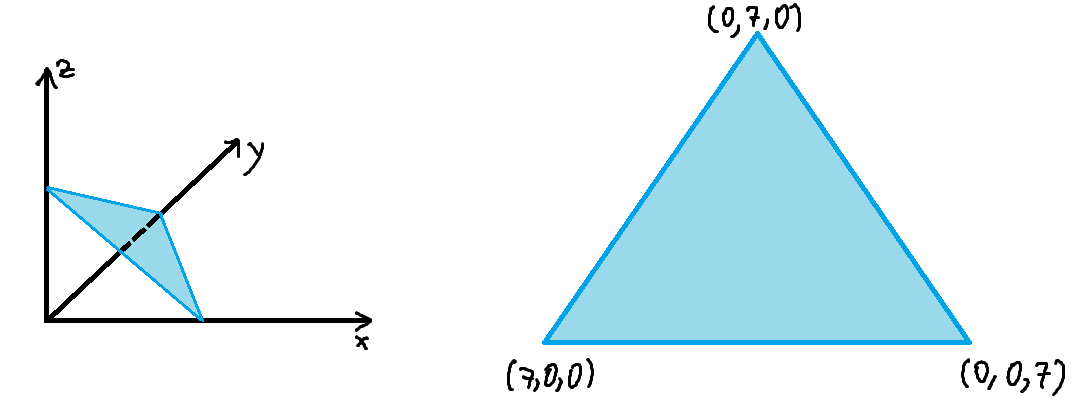
\includegraphics[scale=0.6]{images/slika1.png}
  \end{center}
  Množica imputacij je v tem primeru trikotnik z oglišči 
  $(4, 2, 1)$, $(1, 5, 1)$ in $(1, 4, 2)$. Torej:
  $$I(\Gamma) = \{\lambda_1 (4, 2, 1) + \lambda_2 (1, 5, 1) + \lambda_3 (1, 4, 2)\ |\ \lambda_1 + \lambda_2 + \lambda_3 = 1,\ \lambda_i \geq 0,\ \forall i\}.$$
  \begin{center}
    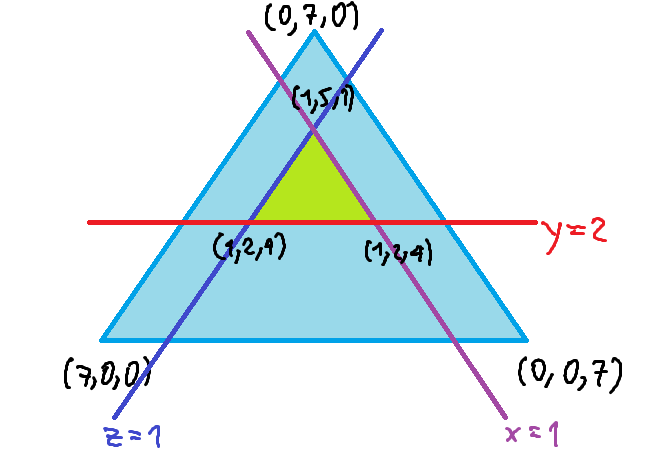
\includegraphics[scale=0.8]{images/slika2.png}
  \end{center}
\end{zgled}

Sedaj definiramo jedro igre $\Gamma = (N, v)$ kot 
$$J(\Gamma) = \{(x_i)_{i \in N} \in \R^n\ |\ \sum_{i \in N} x_i = v(N),\ \forall S \subseteq N:\ \sum_{i \in S} x_i \geq v(S)\}.$$
Očitno je $J(\Gamma) \leq I(\Gamma)$, ker pri imputacijah gledamo le množice $S \subseteq N$, za katere velja $|S| = 1$.
Plačilni vektor je stabilen za $S \subseteq N$, če velja 
$\sum_{i \in S} x_i \geq v(S)$. Jedro so torej vektorji plačil, ki so skupno racionalni 
in stabilni za vse koalicije. Na velikost jedra lahko gledamo kot na mero stabilnosti igre.
V prejšnjem zgledu je recimo 
\begin{align*}
  &J(\Gamma) = \{(x_1, x_2, x_3) \in \R^3\ |\ x_1 + x_2 + x_3 = 7,\ x_1 \geq 1,\ x_2 \geq 2,\ x_3 \geq 1,\\
  &x_1 + x_2 \geq 5, x_1 + x_3 \geq 3,\ x_2 + x_3 \geq 4\}.
\end{align*}
To pa je štirikotnik z oglišči 
$$(2, 4, 1),\ (4, 1, 2),\ (3, 2, 2),\ (3, 3, 1)$$
znotraj ravnine $x_1 + x_2 + x_3 = 7$.
\begin{center}
  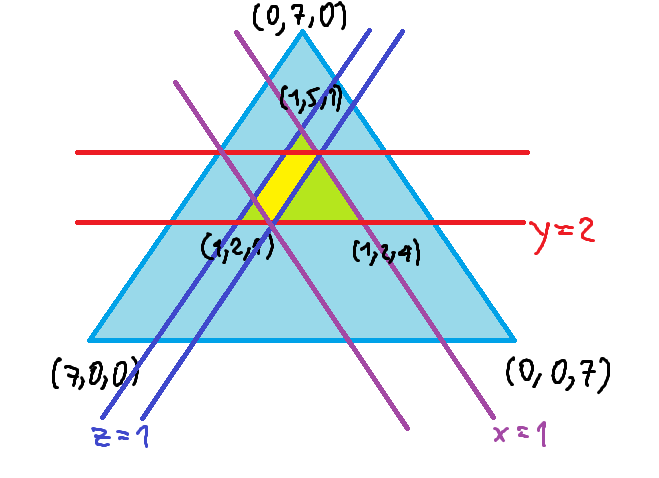
\includegraphics[scale=0.8]{images/slika3.png}
\end{center}

\subsection{Shapleyeva vrednost}

Osnovna ideja je, da iščemo preslikavo 
$$\Phi = \Phi(\Phi_1, \dots, \Phi_n): \{\text{koalicijske igre z $n$ igralci}\} \to \{\text{vektorji plačil}\} \subseteq \R^n,$$
ki bo zadoščala določenim lastnostim. Tem pravimo aksiomi.

\begin{aksiom}[A1]
  Učinkovitost:
  $$\forall v:\ \sum_{i \in N} \Phi(v) = v(N).$$
\end{aksiom}

\begin{aksiom}[A2]
  Simetrija:
  $$\forall v:\ \forall i, j \in N,\ i \neq j:\ \forall S \subseteq N\setminus \{i, j\}:\ v(S \cup \{i\}) = v (S \cup \{j\}) \Rightarrow \Phi_i (v) = \Phi_j (v).$$ 
\end{aksiom}

\begin{aksiom}[A3]
  Dummy player:  
  $$\forall v:\ \forall i \in N:\ \forall S \subseteq N \setminus \{i\}:\ v(S) = v(S \cup \{i\}) \Rightarrow \Phi_i (v) = 0.$$
\end{aksiom}

\begin{aksiom}[A4]
  Aditivnost: 
  $$\forall v, v':\ \forall i \in N:\ \Phi_i (v + v') = \Phi_i (v) + \Phi_i (v').$$
\end{aksiom}

\begin{opomba}
  V nekaterih primerih se četrti aksiom tudi izpusti.
  Takšnih primerov ne bomo srečali.
\end{opomba}

Videli bomo, da obstaja enolična funkcija, ki zadošča tem aksiomom.
Najprej fiksirajmo $v$. Permutacija $\pi: N \to [n]$ določi vrstni red 
igralcev $\pi^{-1} (1), \pi^{-1} (2),\dots, \pi^{-1} (n)$.
Sedaj označimo z $N(\pi, i)$ množico vseh igralcev do vključno igralca $i$.
\begin{align*}
  N(\pi, i) = \{j \in N\ |\ \pi(j) \leq \pi (i)\}.
\end{align*}
Vpeljemo oznako 
$$\Delta(v, \pi, i) = v(N(\pi, i)) - v (N(\pi, i) \setminus \{i\}).$$
Sedaj definiramo 
\begin{equation}
  \Phi_i (v) = \frac{1}{n!} \sum_{\pi \in S_n} \Delta (v, \pi, i) = \mathbb{E} [\Delta(v, \pi, i)].\tag{$5$} \label{eq:5}
\end{equation}

\begin{zgled}
  V prejšnjem zgledu imamo 
  $$
    {\begin{tabular}{c|c|c|c|}
        & $\Delta(v,\cdot, 1)$ & $\Delta(v,\cdot, 2)$ & $\Delta(v,\cdot, 1)$\\
        \hline
        $(1, 2, 3)$ & 1 & 4 & 2\\
        \hline
        $(1, 3, 2)$ & 1 & 4 & 2\\
        \hline
        $(2, 1, 3)$ & 3 & 2 & 2\\
        \hline
        $(2, 3, 1)$ & 3 & 2 & 2\\
        \hline
        $(1, 3, 2)$ & 1 & 4 & 2\\
        \hline
        $(3, 1, 2)$ & 2 & 4 & 1\\
        \hline 
        $(3, 2, 1)$ & 3 & 3 & 1\\
        \hline
    \end{tabular}}        
  $$    
    Torej je $\Phi = \left(\frac{13}{6}, \frac{19}{6}, \frac{10}{6}\right)$ in vidimo, da je res $\frac{13}{6}+\frac{19}{6}+\frac{10}{6} = 7$,
    kot smo hoteli.
\end{zgled}

\begin{trditev}
  Funkcija $\Phi = (\Phi_1, \dots, \Phi_n)$, definirana v \eqref{eq:5}, ustreza Shapleyevim aksiomom.
\end{trditev}

\begin{dokaz}
  Za poljubno permutacijo $\pi \in S_n$ velja 
  $$\sum_{i \in N} \Delta(v, \pi, i) = v(N).$$
  Od tod pa že sledi 
  \begin{align*}
    \sum_{i \in N} \Phi_i (v) &= \sum_{i \in N} \frac{1}{n!} \sum_{\pi \in S_n} \Delta (v, \pi, i)\\
    &= \frac{1}{n!} \sum_{\pi \in S_n} \sum_{i \in N} \Delta (v, \pi, i)\\
    &= \frac{1}{n!} \sum_{\pi \in S_n} v(N)\\
    &= v(N),
  \end{align*}
  zato $\Phi$ ustreza aksiomu o učinkovitosti.
  Sedaj označimo permutacijo $$\pi_{ij} = \begin{cases}
    \pi(k);& \pi(k) \neq i, j\\
    j;& \pi(k) = i\\
    i;& \pi(k) = j
  \end{cases}.$$
  Denimo, da imamo karakteristično funkcijo $v: 2^N \to \R$
  in igralca $i, j \in N$, za katera velja 
  $$\forall S \subseteq N \setminus \{i, j\}:\ v(S \cup \{i\}) = v(S \cup \{j\}).$$
  Potem velja 
  $$v(N(\pi, i)) - v(N(\pi, i) \setminus \{i\}) = v(N(\pi_{ij}, j)) - v(N(\pi_{ij}, i) \setminus \{j\})$$
  in posledično
  $$\forall \pi \in S_n: \Delta(v, \pi, i) = \Delta(v, \pi_{ij}, j).$$
  Ker $\pi_{ij}$ iterira skozi množico vseh permutacij $S_n$, velja naslednje:
  \begin{align*}
    \Phi_i (v) &= \frac{1}{n!} \sum_{\pi \in S_n} \Delta(v, \pi, i)\\
    &= \frac{1}{n!} \sum_{\pi \in S_n} \Delta (v, \pi_{ij}, j)\\
    &= \frac{1}{n!} \sum_{\pi \in S_n} \Delta (v, \pi, j)\\
    &= \Phi_j (v).
  \end{align*}
  S tem smo dokazali, da $\Phi$ ustreza aksiomu o simetriji.
  Sedaj predpostavimo, da za igralca $i$ velja 
  $$\forall S \subseteq N \setminus \{i\}:\ v(S \cup \{i\}) = 0.$$
  Potem je 
  $$\forall \pi \in S_n: \Delta(v, \pi, i) = 0$$ in posledično $\Phi_i (v) = 0$,
  s čemer smo dokazali dummy aksiom.
  Za aksiom o aditivnosti pa moramo opaziti, da velja 
  \begin{align*}
    \Delta(v + v', \pi, i) &= (v + v') (N(\pi, i)) - (v + v')(N(\pi, i) \setminus \{i\})\\
    &= v(N(\pi, i)) - v(N(\pi, i) \setminus \{i\}) + v'(N(\pi, i)) - v'(N(\pi, i) \setminus \{i\})\\
    &= \Delta(v, \pi, i) + \Delta(v', \pi, i).
  \end{align*}
  Potem pa takoj sledi 
  \begin{align*}
    \Phi_i (v + v') &= \frac{1}{n!} \sum_{\pi \in S_n} \Delta(v + v', \pi, i)\\
    &= \frac{1}{n!} \sum_{\pi \in S_n} (\Delta(v', \pi, i) + \Delta(v, \pi, i))\\
    &= \Phi_i(v) + \Phi_i(v'). \qedhere
  \end{align*}
\end{dokaz}

Za izračun Shapleyeve vrednosti $\Phi_i (v)$ si lahko pomagamo z naslednjo trditvijo.

\begin{trditev}
  Za vsakega igralca $i \in N$ velja 
  $$\Phi_i (v) = \sum_{S \subseteq N \setminus \{i\}} \frac{|S|! (n - |S| - 1)!}{n!} (v(S \cup \{i\}) - v(S)).$$
\end{trditev}

\begin{dokaz}
  Naj bo $i \in N$ poljuben igralec. Potem za podano $S \subseteq N \setminus \{i\}$
  obstaja $|S|! (n - |S| - 1)!$ permutacij $\pi$, za katere je $N(\pi, i) = S$.
  Za vsako tako permutacijo je $\Delta(v, \pi, i) = v(S \cup \{i\}) - v(S)$.
  Potem pa iz definicije dobimo 
  \begin{align*}
    \Phi_i (v) &= \frac{1}{n!} \sum_{\pi \in S_n} \Delta(v, \pi, i)\\
    &= \sum_{n \subseteq N \setminus \{i\}} \sum_{\pi \in S_n,\ N(\pi, i) = S} \Delta(v, \pi, i)\\
    &= \sum_{n \subseteq N \setminus \{i\}} \sum_{\pi \in S_n,\ N(\pi, i) = S} (v(S \cup \{i\}) - v(S))\\
    &= \sum_{S \subseteq N \setminus \{i\}} \frac{|S|! (n - |S| - 1)!}{n!} (v(S \cup \{i\}) - v(S)). 
  \end{align*}
\end{dokaz}

\begin{trditev}
  Shapleyeva funkcija je enolično določena.
\end{trditev}

\begin{dokaz}
  Prostor karakterističnih funkcij $v: 2^N \to \R$ je realen vektorski prostor dimenzije $s^N - 1$,
  saj je izomorfen $\R^{2^N \setminus \{\emptyset\}}$.
  Za vsako koalicijo $S \subseteq N$ definiramo karakteristično funkcijo
  $$v_S (T) = \begin{cases}
    1;& S \subseteq T\\
    0;& \text{sicer}
  \end{cases}.$$
  V naslednjem koraku bomo dokazali, da je množica funkcij 
  $B = \{v_S\ |\ S \subseteq N, S \neq \emptyset\}$ baza tega vektorskega prostora.
  Ker $B$ vsebuje $2^N - 1$ elementov, je dovolj pokazati, da so funkcije v $B$ linearno neodvisne.
  Res, naj bo funkcija $v_0$ tista, ki določi ničelno vrednost za vsako koalicijo.
  Če zapišemo 
  $$v_0 = \sum_{S \subseteq N, S \neq \emptyset} \alpha_S \cdot v_S,$$
  potem je očitno, da mora veljati $\alpha_S = 0$ za vse $S \subseteq N$,
  s čimer smo dokazali želeno. Ker vemo, da je $B$ baza vektorskega prostora,
  lahko vsako karakteristično funkcijo pišemo kot 
  $$v = \sum_{v_S \in B} \alpha_S v_S.$$
  Zaradi prvih treh aksiomov velja 
  $$\forall S \subseteq N:\ \Phi_i (\alpha_S V_S) = \begin{cases}
    0;& i \notin S\\
    \frac{\alpha_S}{|S|};& i \in S
  \end{cases}.$$
  Potem pa upoštevamo še četrti aksiom o aditivnosti in dobimo enoličen izraz 
  $$\Phi_i (v) = \Phi_i \left(\sum_{v_S \in B} \alpha_S v_S\right) = \sum_{v_S \in B} \Phi_i (\alpha_S v_S) = \sum_{v_S \in B,\ i \in S} \frac{|\alpha_S|}{|S|}$$
  in $\Phi_i$ je enolično določena.
\end{dokaz}

\begin{zgled}
  Oglejmo si primer, ko je $n \geq 2$ in imamo množico igralcev $N = [n]$.
  Denimo, da je igralec $1$ lastnik firme, preostali igralci pa lahko delajo v njej.
  Denimo, da je dobiček firme $(|S| - 1)b$, kjer je $b > 0$ neko realno število.
  To lahko modeliramo kot koalicijsko igro s karakteristično funkcijo 
  $$v(S) = \begin{cases}
    (|S| - 1)b;& 1 \in S\\
    0;& 1 \notin S
  \end{cases}.$$
  Zanimajo nas Shapleyeve vrednosti igre $\Phi_1, \Phi_2, \dots, \Phi_n$.
  Najprej lahko direktno izračunamo $\Phi_2$; ko je $1$ pred $2$ v permutaciji $\pi$, je $\Delta(v, \pi, 2) = b$,
  sicer pa je $\Delta(v, \pi, 2) = 0$.
  Ker $1$ pride pred $2$ v natanko polovici permutacij, je $\Phi_2 (v) = \frac{1}{n!} \frac{n!}{2} b = \frac{b}{2}$.
  Zaradi simetrije je prav tako 
  $$\Phi_2 = \Phi_3 = \dots = \Phi_n = \frac{b}{2}.$$
  Iz prvega aksioma pa sledi
  $$v(N) = (n - 1)b = \Phi_1 + \Phi_2 + \dots + \Phi_n = \Phi_1 + (n - 1)\frac{b}{2},$$
  torej imamo $\Phi_1 = \frac{b}{2} (n - 1)$.
\end{zgled}

Shapleyeve vrednosti "`merijo"' moč posameznega igralca v polni koaliciji, zato jih včasih uporabimo za to,
da določimo, koliko naj "`dobi'" posamezen igralec.
Shapleyeve vrednosti so pogosto uporabne za merjenje moči  
igralcev v volitvah, ki niso simetrične.
V tem primeru se imenujejo Shapley-Shubikovi indeksi moči.
Za take volitve definiramo 
$$v(S) = \begin{cases}
  1;& \text{če je $S$ dovolj velika, da določi izid volitve}\\
  0;& \text{sicer}
\end{cases}.$$
Shapleyeve vrednosti te igre merijo, za koliko koalicij je vsaj igralec ključen član koalicije.
V tem primeru za vsakega igralca $i \in N$ iščemo 
$$M(i) = \{S \subseteq N \setminus \{i\}\ |\ v(S) = 0, v(S \cup \{i\}) = 1\}$$
in potem 
$$\Phi_i (v) = \sum_{S \in M(i)} \frac{|S|! (n - |S| - 1)!}{n!} (v(S \cup \{i\}) - v(S)).$$
\begin{zgled}
  Denimo, da je v državnem zboru, ki sestoji iz $90$ poslancev,
  natanko $6$ političnih strank, ki imajo $25, 15, 15, 15, 10, 10$ poslancev.
  Predpostavimo, da mora biti vsaj $46$ poslancev za, da sprejmejo odločitev 
  (v Sloveniji se sicer za odločitev izida štejejo le prisotni igralci).
  Če vsaka politična stranka voli skupaj, potem lahko to modeliramo kot igro s šestimi igralci,
  ki jih imenujemo po vrsti $A, B, C, D, E, F$.
  Definirajmo $w(A) = 25$, $w(B) = w(C) = w(D) = 15$ in $w(E) = w(F) = 10$.
  Potem je 
  $$v(S) = \begin{cases}
    1;& \sum_{X \in S} w(X) \geq 46\\
    0;& \sum_{X \in S} w(X) \leq 45
  \end{cases}.$$
  Za koalicijsko igro, ki je določena s to karakteristično funkcijo $v$,
  lahko izračunamo Shapleyeve vrednosti in dobimo 
  $$\Phi_A = \frac{19}{60},\qquad \Phi_B = \Phi_C = \Phi_D = \frac{9}{60},\qquad \Phi_E = \Phi_F = \frac{7}{60}.$$
  Vidimo, da te vrednosti ne naraščajo linearno glede na število poslancev v stranki, ampak upoštevajo,
  za katere koalicije je vsaka stranka ključen član koalicije.
  Takoj lahko vidimo tudi, da velja 
  $$\Phi_A + \Phi_B + \Phi_C + \Phi_D + \Phi_E + \Phi_F = 1.$$
\end{zgled}


\end{document}